\documentclass[lettersize,journal]{IEEEtran}
\usepackage{amsmath,amsfonts}
\usepackage{algorithmic}
\usepackage{array}
\usepackage[caption=false,font=normalsize,labelfont=sf,textfont=sf]{subfig}
\usepackage{textcomp}
\usepackage{stfloats}
\usepackage{url}
\usepackage{verbatim}
\usepackage{graphicx} 
\usepackage{bm}
\usepackage{algorithm}
\usepackage{booktabs}
\usepackage{tabularx}
\usepackage{bm}
\usepackage{placeins}
\usepackage{xcolor}
\usepackage{amssymb}
% ---- revision marking: all text added in this revision is typeset in red ----
\newcommand{\rev}[1]{{\color{red}#1}}
\newenvironment{revblock}{\par\color{red}}{\par}
% ---- text changed in the first revision (blue in the previous version) stays blue ----
\newcommand{\blu}[1]{\texorpdfstring{{\leavevmode\color{blue}#1}}{#1}}
\usepackage[backend=biber, style=numeric, sorting=none]{biblatex}
\addbibresource{bare_jrnl_new_sample4_c123rev.bib}
\usepackage[colorlinks=true, linkcolor=blue, citecolor=blue, urlcolor=blue]{hyperref}
\begin{document}

\title{A Generative Pipeline for 3D Character Animation with Skeleton-free Mesh and Motion Modeling}
\author{Zhigang Tu,~\IEEEmembership{Senior Member,~IEEE,}
        ~Hequan Wang,       
        ~Jiaxu Zhang,
        ~Shaoli Huang,
        ~Junsong Yuan,~\IEEEmembership{Fellow,~IEEE,}
        ~Bo Du,~\IEEEmembership{Senior Member,~IEEE}

\IEEEcompsocitemizethanks{\IEEEcompsocthanksitem Zhigang Tu, Hequan Wang, and Jiaxu Zhang are with the State Key Laboratory of Information Engineering in Surveying, Mapping and Remote Sensing, Wuhan University, Wuhan 430072, China.

\textit{Corresponding
author: Hequan Wang, Jiaxu Zhang and Bo Du (Email: wanghequan@whu.edu.cn, zjiaxu@whu.edu.cn, dubo@whu.edu.cn)}.
\IEEEcompsocthanksitem Shaoli Huang is with Tencent AI Lab, Shenzhen 518063, China.
\IEEEcompsocthanksitem Junsong Yuan is with the Computer Science and Engineering Department, University at Buffalo, Buffalo, NY 14228, USA.
\IEEEcompsocthanksitem Bo Du is with the School of Computer Science, Wuhan University, Wuhan 430072, China.
}
}
% The paper headers
\markboth{IEEE TRANSACTIONS ON PATTERN ANALYSIS AND MACHINE INTELLIGENCE}%
{Tu \MakeLowercase{\textit{et al.}}: A Generative Pipeline for 3D Character Animation with Skeleton-free Mesh and Motion Modeling}


%\IEEEpubid{0000--0000/00\$00.00~\copyright~2023 IEEE}
% Remember, if you use this you must call \IEEEpubidadjcol in the second
\maketitle
\begin{abstract}
Creating an animated 3D character from language involves generating a shape and generating a motion, and the two are almost always built as separate systems that communicate through a finished mesh. This is convenient but structurally wrong: a generator that never sees how its output will be deformed has no reason to produce geometry that deforms well, and the resulting assets routinely break when driven. In this work we present TapMeMo, which replaces that hand-off with a representation shared by both stages. Its central object is a continuous \textit{handle field} that maps any point of space to a distribution over a fixed set of deformation handles. The field is queried at the 3D Gaussians while the character is being generated and at the mesh vertices once it has been extracted, so the deformation structure is carried by the generative representation rather than recovered afterwards by a rigging stage, and no skeleton, template or fixed topology is required anywhere. Two coupling terms make the generator serve the animator: the 2D prior is distilled under motion sampled from the motion model instead of in the rest pose alone, and the expected non-rigidity under that motion distribution is penalised during generation. Both route the generative gradient through the deformation operator, so the mixed second derivative between the two stages, which vanishes identically for a cascade, no longer does; the canonical rest pose then follows as a surrogate for aligning the generator with the support of the motion model rather than being assumed. Training needs neither handle annotations nor text--motion pairs for non-human characters. Besides the usual comparisons against recent rig-free, auto-rigging and feed-forward 4D systems, we report a factorial estimate of the interaction between the two stages, which measures the inseparability that a two-system pipeline cannot produce.
\rev{Routing a gradient to the handle field is, however, not the same as making it informative. We show that the rest-pose objective carries exactly zero Fisher information about the field and cast handle prediction as system identification: under small probing motions the information is second order, linear in the probe covariance, and non-singular if and only if every part boundary is persistently excited, which yields a per-boundary Cram\'er--Rao certificate and an excitation-design objective for the motion model. A frozen articulation prior, trained only on static rigged assets and SMPL bodies without any 4D mesh sequence, acts as the sensor and recovers the correct part partition on 86--92\% of test limbs, including non-human characters, against at most 74\% for image and video diffusion priors; none of the priors we tested, 2D or 3D, reliably locates a joint along a limb. Without any observation of motion, as for a generated character, it lowers the boundary error of a geometric rig by 12\% on held-out characters, a quarter of what an exact sensor achieves. When the deformed vertices can be observed, the identification is amortised into a feed-forward predictor whose 84\,ms refinement is more accurate than the 510\,ms per-character teacher. In the factorial test, applying the animatability prior to 32 generated characters lowers the failure rate of our animator from 27\% to 15\% and does not improve AnimateAnyMesh, an interaction whose 95\% interval excludes zero, whereas smoothing of the same size leaves our failure rate unchanged.}

\end{abstract}

\begin{IEEEkeywords}
3D Character Animation, Skeleton-free Motion Modeling, Handle Field, Animatable 3D Generation, Motion Generation, Text-driven Animations\rev{, Rig Identification, Fisher Information, Score-based Sensing}.
\end{IEEEkeywords}

\section{Introduction}
\IEEEPARstart{T}{he} advent of 3D animation technology has revolutionized the digital world, providing a vibrant platform for storytelling and visual design. However, traditional animation methods remain complex and time-consuming, making them less accessible to newcomers. Learning-based techniques have since decomposed the problem into tasks that are each solved well in isolation: mesh generation \cite{lei2023s, chen2024meshanything, siddiqui2024meshgpt}, auto-rigging \cite{xu2020rignet, xu2022morig, wang2025foundation}, and motion generation \cite{guo2020action2motion,zhang2024motiondiffuse}. The usual way to obtain an animation is to run them in sequence. Our starting observation is that this sequence, and not the quality of its individual stages, is what limits the result: the only thing passed from one stage to the next is a finished mesh, so the generator is never informed about the deformation it will have to support, and the animator can only work with whatever geometry it is handed. Animation quality is therefore decided by a stage that is blind to the objective it is being judged on.

Firstly, existing 3D mesh generation methods \cite{zhang2024clay, weng2025scaling} use text prompts or images as references to create 3D assets for industries such as gaming, film, and AR/VR. However, the generated assets are typically treated as static objects, making it difficult to produce dynamic animations. Moreover, while some methods focus on animatable 3D human generation \cite{yu2023monohuman, wen2024gomavatar}, their results are restricted to pre-rigged human models and cannot generate diverse meshes for a broad spectrum of 3D characters. In contrast, our work addresses a more challenging problem: generating diverse character meshes and animating them through a general pipeline. To enable this, a pose-aware mesh generation model is required to produce character meshes in a consistent rest-pose, thereby facilitating subsequent motion control and synthesis.

Secondly, auto-rigging methods have sought to enable mesh deformation control by skeletonizing and rigging 3D characters using optimization techniques \cite{baran2007automatic} or deep learning models \cite{xu2020rignet, xu2019predicting}. However, these approaches often generate varying skeleton structures for different characters, making it difficult to establish a uniform motion representation for animation. Some methods have proposed using predefined skeleton templates for rigging characters \cite{liu2019neuroskinning, li2021learning}, but they struggle to accommodate meshes with significant variations in shape and topology. As a result, the rigging process frequently requires manual adjustments or custom motions, ultimately limiting the potential for fully automated motion synthesis.

Finally, existing motion generation methods \cite{zhang2024motiondiffuse,tevet2022human,chen2022executing,zhang2024modular} enhance animation by utilizing the SMPL model \cite{loper2015smpl}, a parametric 3D representation of the human body with a standardized skeletal rigging system. However, these approaches oversimplify the process by assuming a fixed mesh topology and skeletal structure, making them ineffective for characters without skeletons. This fundamental limitation greatly restricts the ability to generate motions for diverse, non-rigged 3D characters. \blu{Recent work relaxes the fixed-skeleton assumption: AnyTop~\cite{gat2025anytop}
generates motion for characters of arbitrary skeletal topology by encoding the joint
hierarchy and joint names, and is trained on animal motion capture data. It nevertheless
requires a skeleton as input, so the setting of an unrigged generated mesh remains open.} Additionally, most motion datasets focus on humanoid figures, further constraining the applicability of data-driven techniques to non-standard character designs. Therefore, a significant challenge lies in extending motion generation models from human to non-human characters, enabling the model to accurately perceive their geometry even in the absence of pre-rigged skeletons.

To address these limitations, we present Text-driven Animation Pipeline with skeleton-free Mesh and Motion modeling (TapMeMo), which produces realistic, anthropomorphic motion on a wide range of skeleton-free 3D characters, as illustrated in Figure \ref{fig:teaser}. TapMeMo takes natural language descriptions or reference images as input and returns a character together with its animation. What distinguishes it from running a generator and an animator back to back is that both stages read and write the same object: a continuous \textit{handle field} that assigns every point of space a distribution over a fixed set of deformation handles. The field is queried at the 3D Gaussians while the character is being optimised and at the mesh vertices after extraction, so deformation control is part of the generative representation rather than something reconstructed from it. No skeleton, template or fixed topology appears at any point, which is what allows the same machinery to cover characters whose articulation admits no consistent bone hierarchy.

\begin{revblock}
Sharing the field between the two stages raises a question that a cascade never has to
answer: where does the field get its information? A generated character has never moved, and
in its rest pose every handle carries the identity transformation, so the rendering, and
therefore every 2D prior evaluated on it, is the same for every possible field. We make this
precise in Sec.~\ref{sec:sysid}: the rest-pose objective has zero gradient and zero Fisher
information with respect to the field, so the field is not identifiable from appearance at
all. Existing rigging pipelines escape this by importing the missing information from outside
the character --- artist rigs, observed motion, or the joint ranges of a known skeleton --- which
is exactly what a generated character lacks. We therefore treat rigging as \textit{system
identification}: the motion model supplies the excitation, a frozen prior supplies the sensor,
and the field is the unknown. Under small probing motions the information about the field is
second order and linear in the probe covariance; it is non-singular precisely when every part
boundary is persistently excited, which yields both a Cram\'er--Rao certificate for each
boundary and an objective that lets the motion model choose probes that excite the weakest
boundary. Which prior can act as the sensor is an empirical question, and we answer it with a
controlled test: an articulation prior learned from static 3D assets recovers the part
partition on 86--92\% of test limbs, against at most 74\% for image and video priors, while none
of the priors, vision--language models included, reliably locates a joint along a limb (Fig.~\ref{fig:sysid_motivation}). The
per-character identification is finally amortised into the Mesh Handle Predictor, so inference
remains a single forward pass, followed by a short refinement when the deformed character can be
observed.
\end{revblock}


\begin{figure*}[t]
% \vspace{-2mm} % 适当减少上方空白
% \setlength{\abovecaptionskip}{2mm} % 调整 caption 上方间距
% \setlength{\belowcaptionskip}{2mm} % 调整 caption 下方间距
\centering
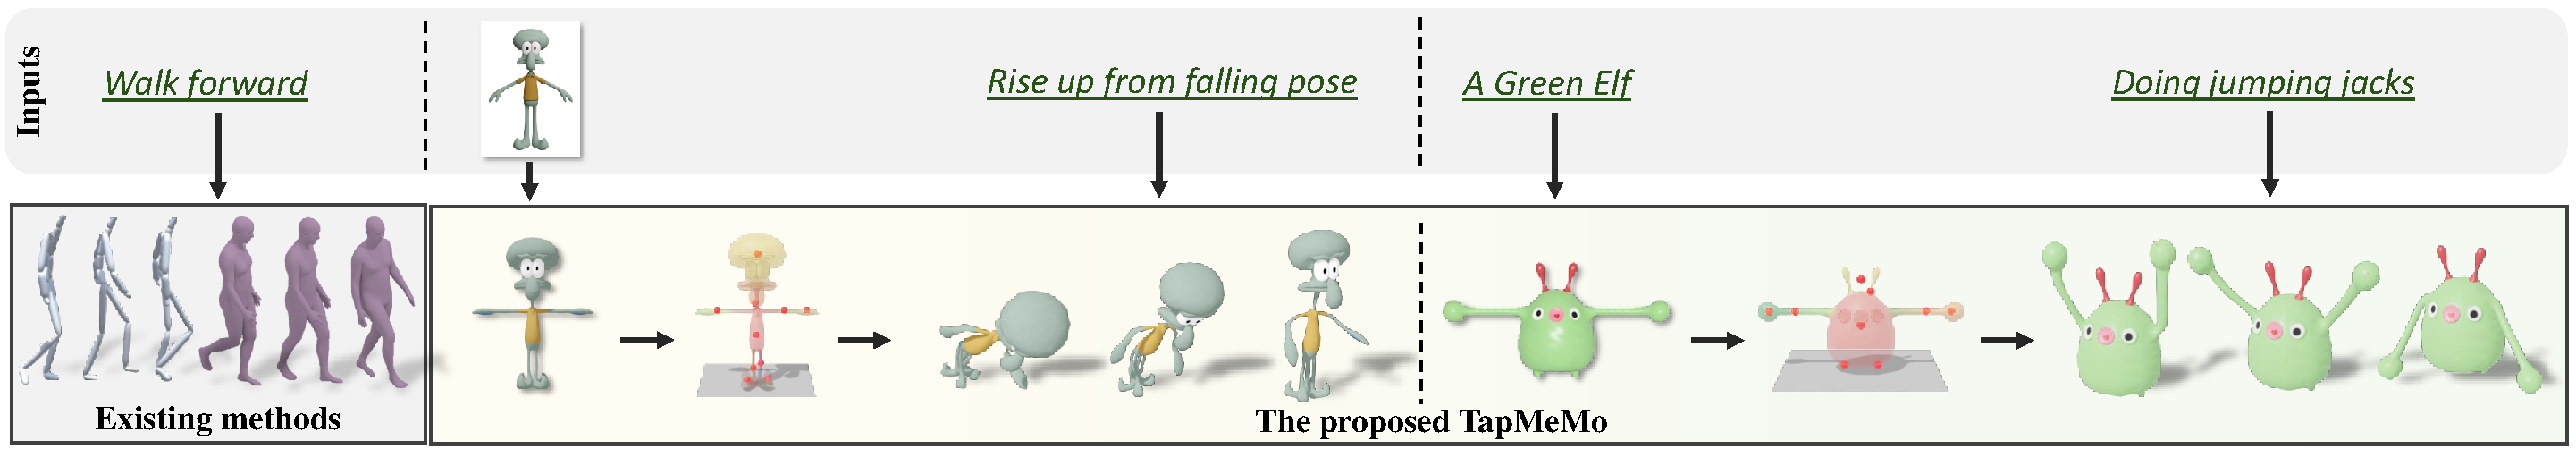
\includegraphics[width=1.0\textwidth]{figure/fig1_.pdf}
\caption{\textbf{We introduce TapMeMo}, a text-driven animation pipeline that generates rest-pose character meshes from images or character prompts, while also producing animations for a wide variety of skeleton-free characters.}
\label{fig:teaser}
\end{figure*}

\begin{figure*}[t]
\centering
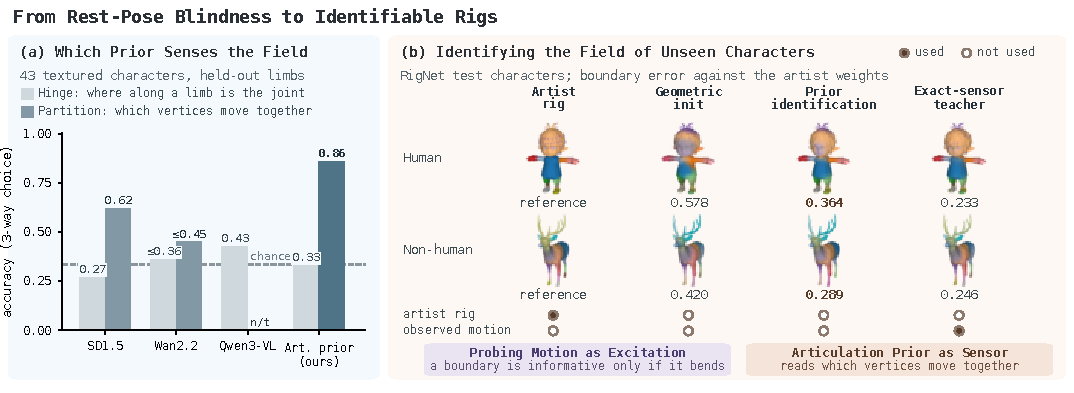
\includegraphics[width=\textwidth]{figure/sysid_motivation.pdf}
\caption{\rev{\textbf{From rest-pose blindness to identifiable rigs.} (a) Accuracy of choosing the
correct one of three candidates on held-out limbs of the 43 textured characters
(Table~\ref{table:sensor}): \textit{hinge} asks where along a limb the joint lies, \textit{partition}
which vertices move with a handle. The Wan2.2 values are the best of 12 readouts and therefore upper
bounds; n/t: not tested. (b) Fields of two RigNet test characters, coloured by handle, with their
boundary error against the artist weights. The articulation prior improves the geometric
initialisation without an artist rig or an observed motion; the exact-sensor teacher observes the
deformed vertices of every probe.}}
\label{fig:sysid_motivation}
\end{figure*}

The Pose-aware Mesh Generator is designed to produce animatable character meshes from text prompts or reference images. Unlike existing methods that generate 3D humans with predefined skeletal rigging systems, our method constrains only the rest-pose of the generated mesh, enabling support for a wide range of characters beyond humans. We introduce a pose-conditioned multi-view adapter for a pre-trained image generation model (e.g., SDXL) to produce multi-view images of the target character. These images are then used to optimize a 3D Gaussian representation initialized by a standard rest-pose. Finally, the character mesh is extracted using the Marching Cubes algorithm. Our Pose-aware Mesh Generator enables character model generation with arbitrary topology and geometric shape, while enforcing a canonical rest-pose to ensure both diversity and animatability.

Given the diversity of generated 3D character meshes, the Mesh Handle Predictor handles mesh deformation control in a unified and consistent manner. Inspired by SfPT \cite{liao2022skeleton}, we utilize a GCN-based network that adaptively locates control handles in the mesh, regulating their movements based on predicted skinning weights. Each predicted handle independently controls its assigned semantic part, while the first handle is fixed as the character's root for global control. Importantly, the module also serves a dual purpose by offering a mesh deformation feature for future shape-aware motion generation.

Shape-aware Motion Diffusion tackles the challenge of understanding mesh structures and generating realistic movements for diverse 3D characters. Since language descriptors serve as an intuitive way for users to interact with computers \cite{manaris1998natural}, we propose a text-driven motion generation model based on the Diffusion Model \blu{\cite{sohl2015deep, ho2020denoising, zhang2024diff, zhang2025visual, zhang2026leveraging}}, which has shown success in generating complex data distributions. Unlike the previous Motion Diffusion Models \cite{zhang2024motiondiffuse,tevet2022human}, our approach produces a universal motion representation that is independent of a character’s skeletal rigging, allowing it to animate a wide variety of characters. A key aspect of our model is the incorporation of Mesh Handle Predictor, which encodes mesh deformation features as an additional condition. It enables motion adaptations tailored to specific meshes meanwhile preserving geometric integrity of the animations. Besides, we employ Linear Blend Skinning to animate mesh using the generated motion and predicted handles.

To address the lack of ground-truth handles and motions for diverse 3D characters, we develop the Pose-aware Mesh Generator as an adapter to the off-the-shelf image generation model SDXL, and propose a novel weakly supervised training strategy for the Mesh Handle Predictor and Shape-aware Motion Diffusion modules in TapMeMo. The proposed method leverages pose constraints, shape constraints, and motion priors as auxiliary supervision signals to improve mesh generation, handle prediction, and motion synthesis.

We assess TapMeMo across a range of animation descriptions and complex 3D characters. Both qualitative and quantitative results demonstrate its effectiveness on both seen and unseen 3D characters. Compared to existing learning-based pipelines, the animations generated by TapMeMo exhibit superior motion fidelity and geometric quality.

Our contributions are listed below.
\begin{itemize}
\item We introduce the \textit{handle field}, a continuous assignment over the ambient space
that is queried both at the Gaussians during generation and at the vertices after extraction.
It is, to our knowledge, the first deformation-control representation that is shared between a
3D generator and a motion model without requiring a skeleton, a template or a fixed topology.
\item We characterise the set of assets on which handle-based driving is exact, the
\textit{drivable manifold} of Eq.~\ref{Eq.mdrv}, and derive its three defining conditions:
the canonical rest pose is the unique identity of the driving operator, since blend skinning
is not compositional (Eq.~\ref{Eq.resid}); the rest-pose rendering objective is blind to the
handle field and invariant to relabelling it (Eq.~\ref{Eq.gauge}), so the T-pose
initialization is the gauge fixing that makes handle channels comparable across characters;
and a uniform, budgeted triangulation is the quadrature condition under which the discrete
handle estimate is consistent with its continuous definition (Eq.~\ref{Eq.quad}). What were
previously presentational choices become necessary conditions with a stated failure mode.
\rev{Each of them is verified separately in Table~\ref{table:drivable}.}
\item We make the generator serve the animator rather than merely precede it, through pose
distillation under generated motion (Eq.~\ref{Eq.posesds}) and an animatability prior
(Eq.~\ref{Eq.anim}). Both route the generative gradient through the deformation operator, so
the mixed second derivative between the two stages no longer vanishes
(Eq.~\ref{Eq.mixed}).
\item We explore a weakly-supervised training strategy that learns the field and
mesh-specific motion with no handle annotations and no text--motion pairs for non-human
characters.
\item We propose a factorial protocol that \textit{measures} the interaction between the two
stages, and report it together with extensive qualitative and quantitative comparisons against
recent rig-free, auto-rigging and feed-forward 4D systems. \rev{Applied to 32 generated
characters, the animatability prior lowers the failure rate of our animator from 27\% to 15\%
without improving AnimateAnyMesh, and the interaction is significant on all three measures,
whereas the rest-pose condition alone produces no measurable interaction
(Table~\ref{table:interaction}). The mesh post-processing interacts with the animator as well:
it lowers the failure rate of our animator on the meshes of all four generators tested and
improves none of three other animators consistently (Table~\ref{table:postproc}).}
\item \rev{We formulate skeleton-free rigging as system identification
(Sec.~\ref{sec:sysid}). We prove that the rest-pose objective carries zero Fisher information
about the handle field, that under probing motion the information is linear in the probe
covariance (Eq.~\ref{Eq.fisherlin}), and that the field is locally identifiable if and only if
every part boundary is persistently excited (Proposition~3). This yields a
per-boundary Cram\'er--Rao certificate and an excitation-design objective, both validated on
human and non-human characters.}
\item \rev{We identify the signal that a frozen prior can contribute to rigging and test it
against every prior family available to us (Sec.~\ref{sec:sensor}). A second-order estimator
reads the prior with forward passes only; an articulation prior trained on static 3D data
recovers the part partition on 86--92\% of test limbs, against at most 74\% for image and video
diffusion priors, which are dominated by the overall magnitude of the deformation. The location
of a boundary along a limb is observable to none of the priors, 2D or 3D, and is left to
geometry. Used as the only sensor, the prior lowers the boundary error of a geometric
initialisation by 12\% on held-out characters, about a quarter of what an exact sensor achieves. On the meshes of four off-the-shelf
generators, sensing the field in this way lowers the failure rate of our animator from 28\% to
20\%, and on non-human characters from 49\% to 35\%.}
\item \rev{We amortise the identification into a feed-forward predictor and add an
identifiability term to motion sampling (Sec.~\ref{sec:amortise}). With exact vertex
observations, the predictor followed by an 84\,ms refinement is more accurate than the 510\,ms
per-character teacher, the same refinement improves UniRig, RigAnything and Puppeteer alike,
and the identifiability term lowers the identification error of motions sampled from the
motion diffusion model by 12\%, at a measured departure from the unguided samples; an
amplitude-matched control shows that the gain is not due to larger motion. These results assume
that the deformed vertices are observed. Without observations, distilling the prior sensor gives
a predictor that needs neither artist rigs nor motion, and the excitation that is best for an
exact sensor brings no gain to the prior sensor.}
\end{itemize}

This work is an \blu{extended version} of our conference paper TapMo \cite{ICLR2024_94154162}. The new contributions include:
\begin{itemize}
\item We lift the discrete handle set of TapMo to the continuous handle field of
Sec.~\ref{sec:field} and identify the drivable manifold of Sec.~\ref{sec:drivable}. This
converts the two elements that a reader would otherwise read as implementation choices, the
T-pose initialization and the decimated, uniformly remeshed output, into the gauge-fixing and
quadrature conditions of the shared representation, each with an equation and a measurable
consequence.
\item We add a generative front end and, more importantly, couple it to the animator: the
Pose-aware Mesh Generator of Sec.~\ref{3Dmesh} optimises handle-rigged Gaussians under motion
sampled from the diffusion model, so the complete system is trained under the single objective
of Eq.~\ref{Eq.unified} instead of as two independent models.
\item We give the rest-pose constraint a derivation rather than a justification
(Eq.~\ref{Eq.align}), and show that it predicts the observed failure mode on characters that
cannot be canonicalised.
\item We evaluate against the 2025--2026 rig-free, auto-rigging and feed-forward 4D
literature, and quantify stage interaction on both human and non-human characters.
\item \rev{We add the identification analysis of Sec.~\ref{sec:sysid}--\ref{sec:amortise},
which explains why the conference version depended on artist rigs, and evaluate it on
Mixamo, on 2,428 heterogeneous RigNet characters and on 43 textured characters, including
negative results for the prior families that do not work as sensors.}
\end{itemize}


\section{Related Work}

\subsection{3D Mesh Generation}
3D mesh generation aims to construct high-quality, animatable 3D assets based on text prompts, reference images, or other perceptual inputs. In recent years, NeRF \cite{mildenhall2021nerf} has been widely applied to 3D reconstruction and generation \cite{yu2021pixelnerf,gao2022mps,chen2023structnerf}, but its optimization process remains highly time-consuming. To improve efficiency, Kerbl et al \cite{kerbl20233d} introduced 3D Gaussian Splatting, which demonstrates significantly superior rendering performance and optimization speed compared to NeRF. Dafei Qin et al \cite{qin2025instant} implemented real-time Gaussian splatting generation for high-quality and real-time facial asset rendering. Furthermore, methods such as SplattingAvatar  \cite{shao2024splattingavatar} and 4D Gaussian Splatting \cite{wu20244d} have extended Gaussian representations to dynamic scenes and human reconstruction, further advancing this line of research.

However, generating animatable 3D meshes remains a significant challenge. Animatable meshes typically require characters to be in a normalized rest-pose to more effectively drive subsequent deformations and motions. Currently, there is still a lack of methods that can directly generate rest-pose for non-human characters in 3D. Most existing methods rely on predefined skeletal rigging strategies, such as parametric human models like SMPL \cite{loper2015smpl} and DreamWaltz-G\cite{huang2025dreamwaltz}, which simplify animation control by enforcing fixed topology and skeleton structures. While effective for standard human scenarios, these approaches are limited in applicability and cannot be easily extended to non-human characters or irregular topologies. Recent work \cite{wang2023zero} has attempted zero-shot pose transfer for stylized 3D characters without skeletal rigging, but they still suffer from limited generalization and insufficient flexibility.  \blu{More recently, TextMesh4D \cite{dai2025textmesh4d} bypasses
rigging entirely by optimising a dynamic mesh directly from text, but it yields one motion
sequence per prompt rather than a rest-pose mesh that can be driven repeatedly.}

To address this, we focus on generating unified rest-pose meshes for a wide variety of characters. Specifically, we integrate a multi-view adapter into the SDXL model, coupled with a pose-constrained ControlNet and a 3D Gaussian-based initialization scheme. This design ensures that the generated characters maintain a normalized rest-pose, enabling skeleton-free motion generation and controllable animation.


\subsection{Motion generation}
Motion generation has long been a fundamental yet persistent challenge in the field of computer graphics \cite{guo2015adaptive}. Traditionally, motion synthesis relied on handcrafted animations or physics-based simulations, both of which demand extensive expertise and manual effort. However, recent advancements in learning-based models have revolutionized this domain, leading to a surge of interest in data-driven motion generation techniques \cite{holden2015learning, holden2016deep}. These state-of-the-art models leverage deep learning to generate realistic movements and often explore various conditioning modalities for human motion synthesis, including but not limited to action labels \cite{guo2020action2motion, petrovich2021action}, audio signals \cite{xu2022freeform, dabral2022mofusion, deng2025stereo}, and text descriptions \cite{zhang2024motiondiffuse,tevet2022human, chen2022executing}.

Text-driven motion generation provides an intuitive, user-friendly way for creating animations via natural language, eliminating the need for 3D rigging expertise or motion capture. \blu{This direction has advanced rapidly in recent years: MoMask
\cite{guo2024momask} and MoGenTS \cite{yuan2024mogents} generate motion by masked modelling over residual
or per-joint quantised motion tokens, MotionStreamer \cite{xiao2025motionstreamer} performs
streaming autoregressive generation in a continuous causal latent space, and MoLingo
\cite{he2025molingo} improves text controllability by aligning the motion latent space with
language.} However, existing methods mainly target human motions and rely on predefined skeletal rigs, limiting their use for non-rigged 3D characters without standard bone-based systems.

Moreover, the availability of large-scale motion datasets has further reinforced this human-centric focus. Many existing datasets provide human motion sequences either as 3D skeleton representations \cite{liu2019ntu, guo2020action2motion, guo2022generating} or as SMPL (Skinned Multi-Person Linear) parameters \cite{mahmood2019amass}. While these datasets have significantly contributed to the development of human motion learning, they predominantly exclude heterogeneous 3D characters, such as creatures, animals, or stylized models, which often lack a standard skeletal structure. As a result, motion generation methods trained on these datasets \cite{zhang2024motiondiffuse,tevet2022human, chen2022executing} struggle to generalize beyond skeletally-rigged human models, making them ill-suited for characters with vastly different mesh topologies and movement constraints.

Recognizing these limitations, our research pioneers a new direction—text-driven motion generation for skeleton-free 3D characters. Unlike the traditional methods that heavily rely on predefined skeletal rigs, our method is capable of handling diverse and complex non-rigged character meshes. Compared to the previous studies, the 3D characters generated by our method are entirely skeleton-free and encompass a wide variety of mesh topologies.

\subsection{Skeleton-Free Mesh Deformation}

Although skeletal rigging systems have long been used in character animation\cite{magnenat1988joint}, creating and skinning skeletons is time-consuming and complex, making it difficult for non-expert users to operate. This has motivated researchers to explore skeleton-free mesh deformation methods that can generate animations without relying on a skeletal structure.

Early approaches in this area mainly relied on manual landmark annotations to drive mesh deformation \cite{ben2009spatial, sumner2004deformation}. While somewhat effective, these methods demanded significant manual effort and struggled to generalize to complex or dynamic motions. More recently, learning-based techniques have emerged. For instance, \cite{yifan2020neural} proposed a neural cage framework for shape deformation that preserves fine geometric details. However, this approach is primarily suited for rigid objects and cannot adequately capture the flexible, articulated nature of animated characters.

Other methods, such as those by \cite{tan2018variational} and \cite{yang2021multiscale}, attempt to embed mesh structures into latent spaces to model deformation primitives. Although promising, these embeddings are usually subject-specific, limiting their generalization across different characters and reducing their effectiveness for tasks like cross-character animation or transfer learning.

The recent SfPT \cite{liao2022skeleton} and HMC \cite{wang2023hmc} generate consistent deformation parts across different character meshes, allowing for pose transfer through the corresponding parts. However, the character's root is ignored in the deformation parts, leading to failure in motion transfer. \blu{AnimateAnyMesh~\cite{wu2025animateanymesh} instead animates an arbitrary mesh from
a text prompt by predicting per-vertex trajectories in a feed-forward manner, which avoids
rigging altogether but provides no reusable deformation control and relies on a
purpose-built 4D dataset.} In this work, inspired by SfPT, we introduce a Mesh Handle Predictor to animate skeleton-free characters in a handle-based manner. This manner represents motion using the translation and rotation of predicted mesh handles, which differs from traditional skeleton-based methods. Our approach diverges from SfPT in two key respects: first, unlike SfPT, we incorporate root handle prediction to enable more intricate motions. Second, our handle predictor also functions to deliver a mesh deformation-aware representation that is crucial for subsequent mesh motion generation.

\subsection{Jointly Generating Geometry, Rig and Motion}
A line of work that emerged concurrently with this manuscript argues that geometry and its
deformation structure should be produced together rather than in sequence, and it is the
closest context for our contribution. On the rigging side, UniRig \cite{zhang2025unirig},
MagicArticulate \cite{song2025magicarticulate}, RigAnything \cite{liu2025riganything} and
Puppeteer \cite{song2026puppeteer} replace the graph-network predictors of
\cite{xu2019predicting,xu2020rignet} with autoregressive transformers over tokenised
skeletons and attention-based skinning, but they still operate as a post-process on a
finished mesh and therefore inherit whatever topological pathologies the generator produced.
AniGen \cite{huang2026anigen} and Rigel3D \cite{rigel3d2026} close this gap by generating
shape, skeleton and skinning weights jointly, as continuous fields or as rig-aware latents,
while RigMo \cite{zhang2026rigmo} learns rigging and motion in a shared latent space from
dynamic mesh sequences. SKDream \cite{xu2025skdream} takes the converse direction and
conditions multi-view and 3D generation \textit{on} a given skeleton.

Our handle field shares the premise of this line --- the deformation structure belongs in the
generative representation --- but differs in three respects. First, it requires no skeleton at
any point, neither as input as in \cite{xu2025skdream} nor as output as in
\cite{huang2026anigen,rigel3d2026}, which is what allows it to cover characters whose
articulation admits no consistent bone hierarchy. Second, it is supervised without any
dynamic ground truth: RigMo \cite{zhang2026rigmo} recovers rig and motion from observed mesh
sequences, whereas our field is learned from static artist rigs and a human motion corpus
only. Third, and most relevant to the present work, the above methods stop at an
animation-ready asset and delegate motion to a separate model such as
\cite{gat2025anytop,mou2026unimate}; we instead let the motion model act back on the
generator, which is the coupling formalised in Sec.~\ref{sec:unified}.

\begin{revblock}
\subsection{Identification, Excitation and Prior-based Sensing}
Whether the parameters of a model can be recovered from data is the classical question of
identifiability: a parametric model is locally identifiable if and only if its information
matrix is non-singular \cite{rothenberg1971identification}, and for dynamical systems this
requires the input to be \textit{persistently exciting} \cite{ljung1999system}. Choosing the
input so that the information matrix is well conditioned is optimal experiment design
\cite{kiefer1960equivalence}, and robotics has long designed excitation trajectories to
identify the inertial parameters of manipulators \cite{gautier1992exciting,swevers1997optimal}.
We transfer this machinery to skinning, where the unknown is the assignment field, the input is
the handle motion, and the sensor is a frozen generative prior.

Read in this language, existing rigging methods are identification with an external excitation:
example poses supplied by an artist \cite{le2012smooth}, observed video frames
\cite{huang2024scgs}, or large corpora of artist rigs
\cite{zhang2025unirig,liu2025riganything,song2026puppeteer}. A character produced by a
generator has none of these, which is why the excitation must be designed rather than
observed. On the sensing side, score distillation \cite{poole2022dreamfusion} reads a frozen
diffusion model through its denoiser; Tweedie's formula \cite{efron2011tweedie} and its
second-order extension \cite{meng2021estimating,manor2024posterior} relate the denoiser and its
Jacobian to the posterior mean and covariance, and antithetic sampling \cite{salimans2017evolution}
removes the odd-order terms of a symmetric perturbation. Finally, it is known that the
likelihood of deep generative models is dominated by low-level statistics of the input rather
than by its semantic content \cite{nalisnick2019deep}, which motivated likelihood-ratio
corrections \cite{ren2019likelihood}; we observe the same effect when a prior is asked to judge
a deformation, and find that, for the part partition, reading the prior at low noise avoids it
where a ratio does not.
\end{revblock}

\section{METHOD}
\begin{figure*}[]
\vspace{-.2cm}
\setlength{\abovecaptionskip}{-.5mm}
\setlength{\belowcaptionskip}{-.3cm}
  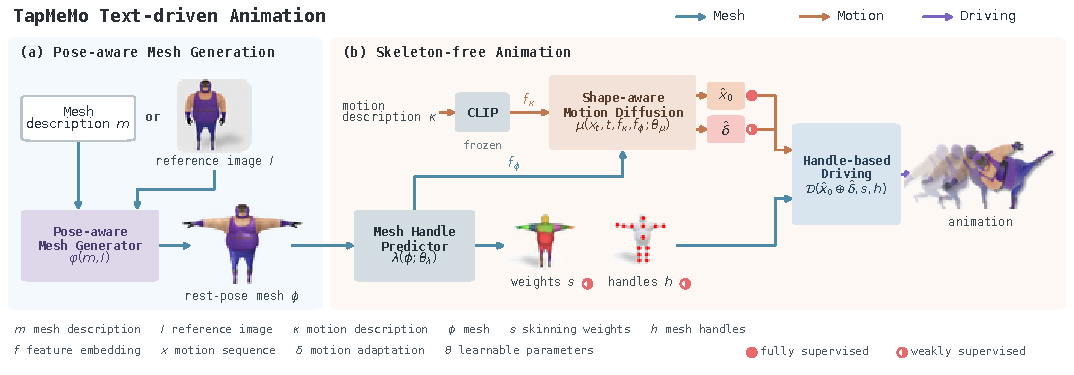
\includegraphics[width=\textwidth]{figure/method_overview.pdf}
  \caption{\textbf{An overview of the TapMeMo pipeline.} Given a user-provided text description or reference image, the \textbf{Pose-aware Mesh Generator} produces the corresponding \textbf{rest-pose} $V^*$ and converts it into a 3D mesh $\phi$. The \textbf{Mesh Handle Predictor} $\lambda(\cdot)$ predicts \textbf{mesh handles} and \textbf{skinning weights} from the user-provided motion description to control the mesh. The \textbf{Shape-aware Motion Diffusion} $\mu(\cdot)$ generates \textbf{text-guided, mesh-specific motion} using the motion description and the \textbf{mesh deformation features} $\mathbf{f}_\phi$ extracted by $\lambda(\cdot)$.}
  \label{fig:Fig2}
\end{figure*}
In this section we first introduce the representation that the whole system is built on, the handle field, and then the two modules that share it: the Pose-aware Mesh Generator and the Shape-aware Motion Diffusion, together with the Mesh Handle Predictor that realises the field. The overall architecture is illustrated in Figure \ref{fig:Fig2}.

As shown in Figure \ref{fig:Fig2}, given a text prompt, which we refer to as the mesh description, or a reference image along with a natural language description of an action, our goal is to generate a realistic character animation that aligns with the described motion $\kappa$.

Specifically, the input mesh description $m$ or reference image $I$ is first fed into the Pose-aware Mesh Generator $\varphi(\cdot)$ , which produces multi-view rest-pose 2D images of the character. The resulting data is used to optimize a 3D Gaussian representation, which is then converted into a rest-pose 3D mesh $\phi$ using the Marching Cubes \cite{lorensen1998marching} algorithm. Crucially, this optimisation is not independent of the animation stage: the Gaussians carry the handle field, and they are optimised under motion sampled from the diffusion model, so the generator is conditioned on the motion description $\kappa$ and on the motion parameters $\bm{\theta}_{\mu}$ as well,
\begin{equation} \label{Eq.1}
\varphi:(m, I, \kappa;\ \bm{\psi}, \bm{\theta}_{\mu}) \;\mapsto (\phi,\ \mathcal{H}_{\bm{\psi}}) .
\end{equation}
The contrast with a cascade, in which the generator would be the skeleton-free counterpart of
$\varphi:(m,I)\mapsto\phi$, is made precise in Sec.~\ref{sec:unified}.

Next, the generated character mesh $\phi$ is passed through the Mesh Handle Predictor $\lambda(\cdot)$, which evaluates the handle field to obtain the assignment $\tilde{\bm{s}}$, from which the handle positions $\bm{h}$ and the deformation weights $\bm{s}$ of the vertices follow. In addition, a low-dimensional mesh deformation feature $\bm{f}_{\phi}$ of the character $\phi$ is extracted to represent the shape of the mesh. Let  $\bm{\theta}_{\lambda}$ denote the learnable parameter of the Mesh Handle Predictor, this process is formulated as:
\begin{equation} \label{Eq.2}
% (\bm{h}, \bm{s}, \bm{f}_{\phi}) = \lambda(\phi; \bm{\theta}_{\lambda}).
\lambda : (\phi; \bm{\theta}_{\lambda}) \mapsto (\tilde{\bm{s}}, \bm{h}, \bm{s}, \bm{f}_{\phi}).
\end{equation}

Subsequently, within the Shape-aware Motion Diffusion module, both the mesh deformation feature $\bm{f}_{\phi}$, which encodes the structural characteristics of the character mesh, and the text embedding $\bm{f}_{\kappa}$, which represents the semantic information of the motion description, are utilized as conditioning inputs. These two modalities guide the diffusion model to generate a motion sequence $\hat{\bm{x}}_{0}$ that is coherent with the textual description and adapted to the specific shape of the input mesh. Additionally, the model predicts a mesh-specific adaptation term $\hat{\bm{\delta}}$, which further refines the generated motion to better fit the underlying geometry.
The text embedding $\bm{f}_{\kappa}$ is obtained using the CLIP model~\cite{radford2021learning}, which effectively captures high-level semantics from natural language descriptions. This inverse diffuse process is formulated as:
\begin{equation} \label{Eq.3}
% (\hat{\bm{x}}_{0}, \hat{\bm{\delta}}) = \mu(\bm{x}_{t}, t, \bm{f}_{\kappa}, \bm{f}_{\phi}; \bm{\theta}_{\mu}),
\mu : (\bm{x}_{t}, t, \bm{f}_{\kappa}, \bm{f}_{\phi}; \bm{\theta}_{\mu}) \mapsto (\hat{\bm{x}}_{0}, \hat{\bm{\delta}}),
\end{equation}

where $\mu(\cdot)$ is the conditional denoiser of the Diffusion Model, and $\bm{x}_{t}$ is the motion of the noising step $t$. $\bm{\theta}_{\mu}$ is the learnable parameter of $\mu(\cdot)$. Following \cite{tevet2022human}, we predict the real motion $\hat{\bm{x}}_{0}$, rather than the noise $\hat{\bm{\epsilon}}_{t}$. Finally, after $T=1,000$ times of the inverse diffuse process, the sum of the generated motion $\hat{\bm{x}}_{0}$ and the adaptation $\hat{\bm{\delta}}$ are applied to the character via a handle-based driving method $\mathcal{D}(\cdot)$ with the predicted $\bm{h}$ and $\bm{s}$.

\subsection{Handle Field: the Shared Deformation Representation} \label{sec:field}
Before describing the two generative modules, we first introduce the representation that
both of them share, because it is this shared representation, rather than the order in which
the modules are executed, that ties them into a single model. Instead of treating
deformation control as a post-processing step applied to a finished mesh, we define a
continuous \textit{handle field} over the ambient space,
\begin{equation} \label{Eq.field}
\mathcal{H}_{\bm{\psi}} : \mathbb{R}^{3} \to \Delta^{K-1},
\qquad
\bm{p} \mapsto \tilde{\bm{s}}(\bm{p}),
\end{equation}
where $\Delta^{K-1}$ denotes the probability simplex, so that $\tilde{s}_{k}(\bm{p}) \geq 0$
and $\sum_{k=1}^{K}\tilde{s}_{k}(\bm{p})=1$ hold at every point. We fix $K=24$ for all
characters, and $\bm{\psi}$ are the parameters of the field, realised by the Mesh Handle
Predictor of Sec.~\ref{sec:handle}.

The essential property of Eq.~\ref{Eq.field} is that it is queried at two different stages of
the pipeline with the \textit{same} parameters $\bm{\psi}$: during generation it is evaluated
at the centers $\bm{x}_{i}$ of the 3D Gaussians, and after mesh extraction it is evaluated at
the mesh vertices $\bar{\bm{V}}_{i}$. Consequently the deformation structure is not recovered
from a finished mesh by a separate rigging stage, it is carried by the very representation
that the generator optimises. Recent work generates geometry together with a skeleton and
skinning weights in a unified field \cite{huang2026anigen,rigel3d2026} or jointly learns
rigging and motion from dynamic mesh sequences \cite{zhang2026rigmo}; our field plays the
same unifying role while requiring neither a skeleton nor dynamic supervision.

\textbf{Handles as the first moment of the field}. The $k$-th handle position is the
field-weighted centroid of the points at which the field is evaluated,
\begin{equation} \label{Eq.moment}
\bm{h}_{k}=\frac{\sum_{i}\tilde{s}_{k}(\bm{p}_{i})\,\bm{p}_{i}}
{\sum_{i}\tilde{s}_{k}(\bm{p}_{i})},
\qquad k=1,\dots,K,
\end{equation}
with $\bm{p}_{i}=\bm{x}_{i}$ during generation and $\bm{p}_{i}=\bar{\bm{V}}_{i}$ afterwards.
A handle is called \textit{active} for a given character if
$\max_{i}\tilde{s}_{k}(\bm{p}_{i})>\tau$ with $\tau=0.1$; inactive handles receive the
identity transformation and are omitted from the visualisations. The number of handles is
therefore fixed, while the number of \textit{active} handles adapts to the character, which
is how a single $K$-dimensional motion representation covers characters of different topology.
The first handle is anchored at the character root and carries the global transformation.

\textbf{Two distinct quantities}. It is important to separate the field output from the
weights that are actually used for deformation, since they play different roles. The field
output $\tilde{\bm{s}} \in \mathbb{R}^{V \times K}$ is an \textit{assignment}: it localises
the handles through Eq.~\ref{Eq.moment} and is the quantity constrained by the supervision
of Sec.~\ref{sec:handle}, and it is defined for all $k=1,\dots,K$ including the root. The
\textit{deformation weights} $\bm{s} \in \mathbb{R}^{V \times (K-1)}$ are then obtained from
the localised handles by a normalised geodesic \blu{radial basis function,}
\begin{equation}\color{blue} \label{Eq.rbf}
s_{i,k}=
\frac{\varrho_{k}\big(d(\bar{\bm{V}}_{i},\bm{h}_{k})\big)}
{\sum_{j=2}^{K}\varrho_{j}\big(d(\bar{\bm{V}}_{i},\bm{h}_{j})\big)},
\qquad
\varrho_{k}(d)=
\exp\Big(-\frac{d^{2}}{2\sigma_{k}^{2}}\Big),
\end{equation}
where \blu{$d(\cdot,\cdot)$ is the geodesic distance on the} mesh \blu{and the bandwidth $\sigma_{k}$ is
predicted} per handle by a separate head of the Mesh Handle Predictor (Sec.~\ref{sec:handle}).
Eq.~\ref{Eq.rbf} ranges over $k=2,\dots,K$ only and guarantees
$\sum_{k=2}^{K}s_{i,k}=1$, so that the local deformation is a convex combination of the
non-root handles, while the root handle acts through the global transformation instead of
through the blend. Whenever a root-related skinning quantity is needed, as in the Root Loss
of Sec.~\ref{sec:handle}, it is the assignment $\tilde{s}_{i,1}$ that is used, never $s_{i,1}$.

\textbf{Motion representation and driving}. The motion of a character is the collection of
handle transformations: local translations $\bm{\tau}^{l} \in \mathbb{R}^{(K-1) \times 3}$,
local rotations $\bm{r}^{l} \in \mathbb{R}^{(K-1) \times 6}$, global translation
$\bm{\tau}^{g} \in \mathbb{R}^{3}$ and global rotation $\bm{r}^{g} \in \mathbb{R}^{6}$, where
all rotations use the continuous 6D parameterisation of \cite{zhou2019continuity}. Writing
$\bm{x}_{0}=\{\bm{\tau}^{l},\bm{r}^{l},\bm{\tau}^{g},\bm{r}^{g}\}$, a point $\bm{p}$ is
driven by the handle-based operator $\mathcal{D}(\cdot)$ as
\begin{equation} \label{Eq.4}
\mathcal{D}(\bm{p};\bm{x}_{0})=
\bm{R}^{g}\Big( \sum_{k=2}^{K} s_{k}(\bm{p})
\big( \bm{R}^{l}_{k}(\bm{p}-\bm{h}_{k}) + \bm{\tau}^{l}_{k} + \bm{h}_{k} \big) \Big)
+ \bm{\tau}^{g},
\end{equation}
where $\bm{R}^{g}$ and $\bm{R}^{l}_{k}$ are the rotation matrices obtained from
$\bm{r}^{g}$ and $\bm{r}^{l}_{k}$. Note that the recentering term $\bm{h}_{k}$ lies inside
the blend, so that every summand is a complete rigid transformation of $\bm{p}$ by handle
$k$ and the result is a convex combination of such transformations. Because each point is
displaced by a blend of handle transformations weighted by its own \blu{weights, a region that
does not host a handle of its own is still driven by the surrounding handles in proportion to
these} weights and deforms continuously between them. Applying $\mathcal{D}$ to the mesh
vertices yields the animated mesh, $\bar{\bm{V}}_{i}^{'}=\mathcal{D}(\bar{\bm{V}}_{i};\bm{x}_{0})$;
applying it to the Gaussian centers yields a deformed generative representation, which is the
mechanism exploited in Sec.~\ref{3Dmesh}.

\subsection{The Drivable Manifold: What the Generator Must Produce} \label{sec:drivable}
The handle field tells us how a character is deformed, but not which characters can be
deformed \textit{correctly}. This subsection answers that question, and the answer is what
turns the 2D-to-3D stage from a preprocessing step into a constrained generation problem.
We show that the driving operator $\mathcal{D}$ of Eq.~\ref{Eq.4} is exact only on a
restricted set of assets,
\begin{equation} \label{Eq.mdrv}
\mathcal{M}_{\text{drv}}=
\Big\{(\phi,\mathcal{H}_{\bm{\psi}})\ :\
\underbrace{\bm{p}_{0}=\bm{x}_{\text{id}}}_{\text{P1}},\
\underbrace{\bm{\psi}\in\mathcal{G}_{0}}_{\text{P2}},\
\underbrace{A_{i}\equiv\bar{A},\ |V|\!\approx\!V^{\star}}_{\text{P3, P4}}
\Big\},
\end{equation}
and that the three conditions are, respectively, the canonical rest pose, a canonical gauge
$\mathcal{G}_{0}$ for the handle indices, and a uniform, budgeted triangulation. None of them
is a matter of taste: each one is the condition under which a specific quantity used by the
motion model is unbiased or well defined. Our generator is then defined as
2D-to-3D generation restricted to $\mathcal{M}_{\text{drv}}$, which is the precise sense in
which it serves the animation stage.

\textbf{P1: the rest pose is the identity of the driving operator.} Linear blend skinning is
not compositional. Let $\bm{a}$ and $\bm{b}$ be two motions and let $\bm{h}^{\bm{a}}_{k}$ and
$s^{\bm{a}}_{k}$ denote the handle positions and weights re-estimated on the configuration
deformed by $\bm{a}$. Applying $\bm{b}$ afterwards gives
$\mathcal{D}(\mathcal{D}(\bm{p};\bm{a});\bm{b})$, which uses
$(\bm{h}^{\bm{a}}_{k},s^{\bm{a}}_{k})$, whereas the motion model is trained to express the
composite displacement as a single application $\mathcal{D}(\bm{p};\bm{b}\!\circ\!\bm{a})$
with the canonical $(\bm{h}_{k},s_{k})$. The two disagree by the composition residual
\begin{equation} \label{Eq.resid}
\mathcal{E}(\bm{a},\bm{b})=
\big\lVert\mathcal{D}(\mathcal{D}(\bm{p};\bm{a});\bm{b})-
\mathcal{D}(\bm{p};\bm{b}\!\circ\!\bm{a})\big\rVert ,
\end{equation}
which is non-zero in general because both the blend weights and the blend centers have moved.
Setting $\bm{a}=\bm{x}_{\text{id}}$, the identity motion, restores
$\bm{h}^{\bm{a}}_{k}=\bm{h}_{k}$ and $s^{\bm{a}}_{k}=s_{k}$, hence
$\mathcal{E}(\bm{x}_{\text{id}},\bm{b})=0$ for every $\bm{b}$. The canonical rest pose is
therefore not a convenient convention but the unique configuration at which driving a
generated asset incurs no composition error; a character generated in an arbitrary pose
$\bm{p}_{0}$ is driven with an irreducible error $\mathcal{E}(\bm{p}_{0},\bm{b})$ that no
amount of motion-model capacity can remove. This also predicts, rather than merely
describes, the failure mode of Fig.~\ref{fig:fig13}.

\textbf{P2: the rest-pose objective cannot learn the handle field, so the initialization must
fix its gauge.} A rendering of the character in its rest pose does not depend on the handle
field at all: the Gaussians are rasterised from $\{\mathbf{x}_i,\mathbf{s}_i,\mathbf{q}_i,
\alpha_i,\bm{\beta}_i\}$ and $\tilde{\bm{s}}_{i}$ enters nowhere. Consequently
\begin{equation} \label{Eq.gauge}
\nabla_{\bm{\psi}}\mathcal{L}^{\text{rest}}_{\text{diff}}=\bm{0},
\qquad
\mathcal{L}^{\text{rest}}_{\text{diff}}(\Theta,\pi\!\cdot\!\bm{\psi})=
\mathcal{L}^{\text{rest}}_{\text{diff}}(\Theta,\bm{\psi})
\quad \forall\pi\in S_{K},
\end{equation}
where $\pi$ permutes the $K$ handle channels. The rest-pose objective is blind to the field
and invariant to any relabelling of the handles, so the field is identifiable at best up to
the symmetric group $S_{K}$, a $K!$-fold ambiguity. This matters because the motion
representation $\bm{x}_{0}$ is index-addressed: $\bm{\tau}^{l}_{k}$ is the translation of the
$k$-th channel, and the motion model is trained with one fixed assignment of channels to
semantic parts. Transferring motion to a newly generated character therefore requires
selecting one specific element of the $S_{K}$ orbit, the canonical gauge $\mathcal{G}_{0}$ of
Eq.~\ref{Eq.mdrv}. Initialising the Gaussians from the joints and bones of a canonical T-pose
performs exactly this selection: each Gaussian is born with the index of the part it was
spawned from, so channel $k$ denotes the same semantic part across every character. A
spherical initialization leaves the gauge undetermined and the handle channels permuted
arbitrarily per character, which is why it breaks cross-character motion transfer even when
the resulting geometry is visually comparable. The rest-pose initialization is thus a
symmetry-breaking device for identifiability, and the two coupling terms of
Sec.~\ref{3Dmesh} are what subsequently give $\bm{\psi}$ a non-zero gradient at all.
\rev{A non-zero gradient is, however, necessary but not sufficient: Sec.~\ref{sec:sysid} shows
that the information it carries about $\bm{\psi}$ is second order in the motion amplitude,
characterises which parts of the field it can determine, and Sec.~\ref{sec:sensor} identifies
which prior can deliver it.}

\textbf{P3: uniform triangulation is the quadrature condition for the handle positions.}
Eq.~\ref{Eq.moment} is a discretisation of a surface integral. The handle position is properly
defined on the continuous surface $\mathcal{S}$ as
\begin{equation} \label{Eq.quad}
\bm{h}_{k}=
\frac{\int_{\mathcal{S}}\tilde{s}_{k}(\bm{p})\,\bm{p}\;\mathrm{d}A(\bm{p})}
{\int_{\mathcal{S}}\tilde{s}_{k}(\bm{p})\;\mathrm{d}A(\bm{p})}
\ \approx\
\frac{\sum_{i}A_{i}\,\tilde{s}_{i,k}\,\bm{p}_{i}}{\sum_{i}A_{i}\,\tilde{s}_{i,k}},
\end{equation}
with $A_{i}$ the barycentric area of vertex $i$. The plain vertex average of
Eq.~\ref{Eq.moment} coincides with this consistent estimator if and only if
$A_{i}\equiv\bar{A}$, that is, only on a uniform triangulation; otherwise the estimated handle
is biased towards densely tessellated regions, with the bias growing with the dispersion of
$\{A_{i}\}$. \rev{A Marching-Cubes surface decimated by QEM is strongly non-uniform (the raw
Marching-Cubes surface is not, see Sec.~\ref{sec:exp}),} so its handles are
systematically displaced, and this displacement propagates into Eq.~\ref{Eq.rbf} and into
every frame of Eq.~\ref{Eq.4}. Isotropic remeshing is therefore the step that makes the
estimator of Eq.~\ref{Eq.moment} consistent; it is a quadrature requirement of our
formulation, not a cosmetic clean-up. \rev{The area weights of Eq.~\ref{Eq.quad} remove the
bias on any triangulation, so remeshing is required wherever the plain vertex average is used,
as in the TapMo predictor, whose handles are plain field-weighted vertex averages.} The same uniformity governs Eq.~\ref{Eq.rbf} through the
discrete geodesic distance, whose accuracy degrades as the minimum triangle angle shrinks and
sliver triangles appear.

\textbf{P4: the vertex budget normalises the field across characters.} The field is realised
by a graph network whose receptive field spans a fixed number of hops. The surface fraction
covered by those hops scales with $|V|^{-1/2}$, so if $|V|$ varies by orders of magnitude
across characters, channel $k$ aggregates evidence from regions of incomparable physical
extent and the assignment ceases to be comparable across characters. Decimating every
character to a common budget $V^{\star}$ with a bounded geometric error, which is what the
quadric error metric provides, makes the receptive field a fixed fraction of the surface and
is the condition under which a single set of $K$ channels is meaningful across heterogeneous
characters. Reducing the face count is, in this formulation, a statement about the
identifiability of the shared representation rather than a concession to rendering cost.

Taken together, P1--P4 say that the asset handed to the motion model must sit at the identity
of the driving operator, in a canonical channel gauge, on a uniform and budgeted
triangulation. The next subsection describes a generator built to satisfy exactly these
constraints, and Sec.~\ref{sec:exp} verifies each of them separately.

\subsection{Pose-aware Mesh Generator} \label{3Dmesh}

\blu{This module is supervised only in image space and uses no 3D ground truth: the
Camera Adaptor is trained with a diffusion noise-prediction loss on multi-view renderings,
and the per-character 3D Gaussians are then optimised by score distillation from a frozen
2D prior.} Previous methods for generating 3D meshes from text descriptions or single-view reference images often face challenges such as inconsistent rest-pose and topological distortions, which severely limit the generality and animatability of the auto-generated meshes. Although some methods typically introduce predefined mesh topologies and skeletal structures, such as SMPL, to enhance animation performance, their generalization capability remains limited, particularly when dealing with non-human characters.
\begin{figure*}[]
\vspace{-.2cm}
\setlength{\abovecaptionskip}{-.5mm}
\setlength{\belowcaptionskip}{-.3cm}
  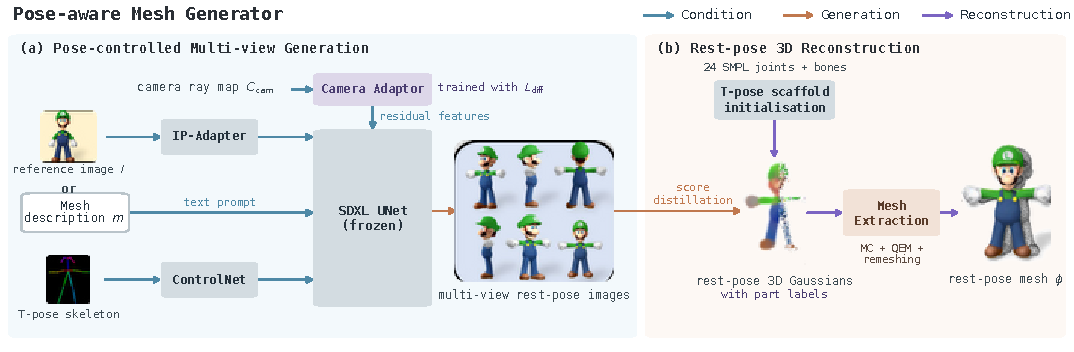
\includegraphics[width=\textwidth]{figure/method_generator.pdf}
  \caption{\textbf{An overview of the Pose-aware Mesh Generator.} We trained a Pose-controlled Camera Adaptor. Within the SDXL framework, given a mesh description  $m$ or a reference image $I$, we incorporate camera view information as a conditional input $C_{\text{cam}}$ to generate multi-view images, while leveraging ControlNet to normalize the character's pose to a standard rest-pose. These multi-view images are then used to optimize the 3D Gaussian representation, ultimately producing a high-quality mesh in the standard rest-pose.
}
  \label{fig:Fig3}
\end{figure*}

We draw inspiration from the recent advances in the domains of multi-view generation and high-fidelity 3D model reconstruction, and propose the Pose-aware Mesh Generator, as illustrated in Figure \ref{fig:Fig3}. This approach not only ensures that the generated meshes strictly adhere to the canonical rest-pose constraint but also provides a reliable foundation for the subsequent mesh handle prediction and skeleton-free motion generation for non-rigid characters.

Specifically, we train a pose-controlled camera adapter to provide multi-view geometric constraints during the 3D Gaussian optimization process. Given a mesh description $m$ or a reference image $I$, this module, combined with the pose-conditioned SDXL model, generates a set of multi-view images $I_v$, where $v$ denotes the viewpoint index. All generated images maintain a standardized rest-pose, serving as reliable references for the subsequent 3D Gaussian optimization. We observe that incorporating pose-aware conditioning not only significantly reduces local shape errors and cross-view inconsistencies, but also preserves the overall spatial structure and fine-grained details of the character.

Next, to accelerate the 3D Gaussian optimization process and ensure that the character maintains a standardized rest-pose, we do not initialize the 3D Gaussian distribution as a sphere. Instead, we directly initialize the 3D Gaussian representation using the standardized rest-pose. We also adopt the representation proposed by Gaussian Splatting \cite{kerbl20233d}, where the location of each Gaussian can be described by a center $x \in \mathbb{R}^3$, a scaling factor $s \in \mathbb{R}^3$, and a rotation quaternion $\mathbf{q}\in \mathbb{R}^4$.

Finally, to extract the geometry of the mesh, we apply the Marching Cubes algorithm \cite{lorensen1998marching}. After obtaining the mesh geometry, we back-project the character’s multi-view images onto the mesh surface and bake them as textures. The resulting mesh $\phi$ not only strictly adheres to the static rest-pose constraint but also preserves detailed information from the multi-view renderings, ensuring high consistency in both geometry and texture, thus providing a solid foundation for subsequent shape-aware motion generation.

\textbf{Pose-controlled Camera Adaptor}. The core idea is inspired by ControlNet
\cite{zhang2023adding}, but with notable differences: \blu{the Camera Adaptor is a
lightweight convolutional encoder rather than a trainable copy of the SDXL UNet, and it
borrows only the idea of injecting multi-scale residual features into a frozen} backbone.
Within the SDXL-based framework, we incorporate camera view information
\blu{through this} encoder, ensuring that the generated images strictly correspond to
the specified camera viewpoints while preserving the semantic information from the original
text prompts and reference images.

We use the camera view information as a conditional input
\(C_{\text{cam}} \; (C_{\text{cam}} \in \mathbb{R}^{n \times c \times h \times w})\),
\blu{which is a per-pixel camera ray map rather than the raw extrinsics:} \(n\) \blu{is the number of
generated views, and for each view we compute at every pixel the ray origin and the ray
direction in world coordinates, giving} \(c=6\) \blu{channels, while} \(h \blu{\times w}\) \blu{is the spatial
resolution of the SDXL latent. Encoding the camera as a dense ray map instead of a global
rotation and translation vector keeps the condition spatially aligned with the latent, which
is what allows it to be added to the UNet features directly.}
This input is processed by a lightweight convolutional encoder to generate multi-scale
residual features, which are then injected into the corresponding layers of the UNet
\blu{by element-wise addition: the residual feature produced at each scale is added to
the output of the SDXL UNet encoder block with the same spatial resolution, without any
learnable scaling factor or attention module,} enabling precise control over the generated
image's viewpoint.
During training, we keep the weights of the SDXL backbone frozen and only optimize the Camera Adapter, 
allowing it to learn how to map camera view conditions into the latent space, thus guiding the generated images to strictly follow the target camera viewpoint. At the same time, we use the diffusion noise prediction loss:

\begin{equation} \label{Eq.Ldiff}
L_{\text{diff}} = \mathbb{E} \Big[ \| \epsilon - \hat{\epsilon}(z_t, t, C_\text{text}, C_\text{cam}) \|_2^2 \Big],
\end{equation}
where 
\(\epsilon\) is the randomly sampled Gaussian noise, 
\(\hat{\epsilon}(\cdot)\) is the noise predicted by the UNet, 
\(z_t\) is the latent representation of the input image at timestep \(t\), 
\(C_\text{text}\) is the text condition embedding, 
and \(C_\text{cam}\) is the camera view condition encoded by the Camera Adapter. This loss ensures that the model predicts the correct noise given the camera conditions, thereby achieving alignment from camera to image.

Meanwhile, our trained Camera Adapter is based on SDXL, making it compatible with SDXL-based ControlNet and IP-Adapter. When used in conjunction with ControlNet, it enables control over the character's rest-pose. 
When combined with IP-Adapter, it can generate corresponding multi-view images based on an input reference image \(I\).

\textbf{Rest-pose Initialized 3D Gaussian \blu{Optimization}}.  Gaussian Splatting represents 3D scenes using a collection of 3D Gaussians, demonstrating significant efficiency advantages in image-to-3D generation tasks. We adopt the Gaussian representation proposed by Kerbl et al.~\cite{kerbl20233d}, where each Gaussian is described by a center point $\mathbf{x}\in \mathbb{R}^3$, a scaling factor $\mathbf{s}\in \mathbb{R}^3$, and a rotation quaternion $\mathbf{q}\in \mathbb{R}^4$. We also store an opacity value $\alpha \in \mathbb{R}$ and a color feature $\bm{\beta} \in \mathbb{R}^3$ for volumetric rendering. All the above optimizable parameters are represented by $\Theta$  , where $\Theta_i = \{\mathbf{x}_i, \mathbf{s}_i, \mathbf{q}_i, \alpha_i, \bm{\beta}_i\}$ denotes the parameters of the $i$-th Gaussian. Unlike previous methods that initialize 3D Gaussians within a spherical volume, to accelerate the optimization process and ensure that the character maintains a standardized rest-pose, we initialize the Gaussians directly based on the normalized rest-pose.

Specifically, we first select the 24 primary skeletal joints from the SMPL model, each represented by a three-dimensional coordinate. For each joint, we take the joint as the center, define a radius $r$, and generate several small Gaussian distributions within its surrounding region to cover the local space around the joint. We emphasise that the T-pose skeleton is used here only as a \textit{labelled scaffold}, never as a rigging structure: it is discarded after initialization, it imposes no bone hierarchy on the generated character, and the number of channels it labels, $K=24$, is the same for characters whose articulation has nothing in common with a human skeleton. Its role is the gauge fixing of P2: because the rest-pose rendering objective is blind to the handle field (Eq.~\ref{Eq.gauge}), the correspondence between channel $k$ and a semantic part cannot be learned from images and must be injected at initialization, and this is the only mechanism in the pipeline that supplies it.

For larger or elongated body parts (such as arms and legs), relying solely on joint-based initialization may lead to discontinuous Gaussian distribution. To address this, we perform linear interpolation between adjacent joints along the skeletal connections and generate additional Gaussian spheres along the bones, ensuring continuous coverage of the entire limb rather than restricting the distribution to joint locations. Through these steps, we finally obtain an initial set of 3D Gaussians based on the rest-pose, which serves as the starting point for subsequent 3D Gaussian optimization. \blu{Because the Gaussians are spawned from the joints and bones of the canonical rest pose,
each Gaussian additionally records the part it originates from. This part information is
retained throughout the optimization and transferred to the extracted mesh, so that every
vertex of the mesh carries a part label, which is used to initialise the} assignment field in
Sec.~\ref{sec:handle}.

Next, we optimize 3D Gaussians under the Pose-controlled Camera Adaptor. The optimization formula is given by:

\begin{equation} \label{Eq.5}
\nabla_{\Theta} L_{\text{diff}} = \mathbb{E}_{t, p, \epsilon} \Big[ w(t) \big( \hat{\epsilon}(z_t, t, C_{\text{text}}, C_{\text{cam}}) - \epsilon \big) \frac{\partial I_p}{\partial \Theta} \Big],
\end{equation}
where \(t\) is the diffusion timestep, \(w(t)\) is the corresponding weighting coefficient for timestep \(t\), and \(p\) denotes the camera parameters of the current viewpoint. \(I_p\) represents the 2D image rendered from the 3D Gaussian parameters \(\Theta\).

\textbf{Handle-rigged Gaussians and Pose Distillation}. Eq.~\ref{Eq.5} constrains the
character only in its rest pose, which is exactly the point at which a generator and an
animator remain two separate systems: nothing in Eq.~\ref{Eq.5} knows how the asset will later
be deformed. We therefore bind the handle field of Sec.~\ref{sec:field} to the Gaussians and
distil the 2D prior under \textit{generated motion} rather than in the rest pose alone.
Concretely, every Gaussian is augmented with its field value,
$\Theta_i=\{\mathbf{x}_i,\mathbf{s}_i,\mathbf{q}_i,\alpha_i,\bm{\beta}_i,
\tilde{\bm{s}}_i\}$ with $\tilde{\bm{s}}_i=\mathcal{H}_{\bm{\psi}}(\mathbf{x}_i)$, and the
driving operator of Eq.~\ref{Eq.4} is applied directly to the Gaussian centers, with the
covariance rotated consistently \cite{dabhi2026rat4d},
\begin{equation} \label{Eq.gsdeform}
\mathbf{x}_i^{n}=\mathcal{D}(\mathbf{x}_i;\bm{x}^{n}),
\qquad
\Sigma_i^{n}=\bm{R}_i^{n}\,\mathrm{diag}(\mathbf{s}_i^{2})\,\bm{R}_i^{n\top},
\end{equation}
where $\bm{R}_i^{n}=\bm{R}^{g}\sum_{k=2}^{K}s_{k}(\mathbf{x}_i)\bm{R}^{l}_{k}$ is the blended
rotation at Gaussian $i$ in frame $n$. Sampling a motion
$\bm{x}\sim p_{\mu}(\cdot\mid\bm{f}_{\kappa},\bm{f}_{\phi})$ from the \textit{frozen} Shape-aware
Motion Diffusion of Sec.~\ref{sec:motion} and rendering the deformed Gaussians gives the pose
distillation gradient
\begin{equation} \label{Eq.posesds}
\nabla_{\Theta}\mathcal{L}_{\text{pose}}=
\mathbb{E}_{t,p,\epsilon,n}\Big[
w(t)\big(\hat{\epsilon}(z_{t}^{p,n},t,C_{\text{text}},C_{\text{cam}})-\epsilon\big)
\frac{\partial I_{p}^{n}}{\partial\mathcal{D}(\Theta;\bm{x}^{n})}
\frac{\partial\mathcal{D}(\Theta;\bm{x}^{n})}{\partial\Theta}\Big],
\end{equation}
in which $I_{p}^{n}$ is the frame-$n$ rendering from view $p$ and the text condition
$C_{\text{text}}$ is the concatenation of the mesh description $m$ and the motion description
$\kappa$. The factor $\partial\mathcal{D}/\partial\Theta$ is the formal content of the claim
that the generator serves the motion model: the update direction of the generative parameters
is routed through the deformation operator of the animation stage, so a geometry that cannot
be driven cleanly is penalised at generation time rather than discovered afterwards.

\textbf{Animatability Prior}. The same coupling can be imposed without a 2D prior, by
penalising the expected non-rigidity of the asset under the motion distribution,
\begin{equation} \label{Eq.anim}
\mathcal{R}_{\text{anim}}(\Theta,\bm{\psi})=
\mathbb{E}_{\bm{x}\sim p_{\mu}(\cdot\mid\bm{f}_{\kappa})}
\Big[\sum_{n=1}^{N}\sum_{(i,j)\in\Phi}
\big(\lVert\mathbf{x}_{i}^{n}-\mathbf{x}_{j}^{n}\rVert-
\lVert\mathbf{x}_{i}^{0}-\mathbf{x}_{j}^{0}\rVert\big)^{2}\Big],
\end{equation}
where $\Phi$ is the edge set of the triangulation induced on the Gaussians by their
$k$-nearest-neighbour graph. Eq.~\ref{Eq.anim} turns local rigidity from a quantity that is
merely \textit{measured} after animation into a term that the generator \textit{optimises},
which is what makes the resulting rest-pose asset animation-ready by construction instead of
by post-processing.

\textbf{Why the rest pose is required, not preferred}. Finally, the canonical rest pose itself
follows from the same coupling rather than from an aesthetic convention. The motion model
of Sec.~\ref{sec:motion} is conditioned on the deformation feature $\bm{f}_{\phi}$ and is
trained on a fixed set of characters, so its conditional $p_{\mu}(\bm{x}\mid\bm{f}_{\phi})$
is only reliable on the support $p_{\text{train}}(\bm{f}_{\phi})$ induced by that set. An
unconstrained generator places $\bm{f}_{\phi}$ off this support and forces the motion model to
extrapolate, which is the actual origin of the distortion reported in Sec.~\ref{sec:exp}.
Writing $q_{\varphi}$ for the distribution of deformation features induced by the generator,
the generator objective is therefore
\begin{equation} \label{Eq.align}
\min_{\varphi}\ \
\mathbb{E}_{m,I}\big[-\log p_{\text{2D}}\big(\varphi(m,I)\big)\big]
\ +\ \beta\,\mathrm{KL}\big(q_{\varphi}(\bm{f}_{\phi})\,\big\|\,p_{\text{train}}(\bm{f}_{\phi})\big),
\end{equation}
and constraining the output to the canonical rest-pose manifold is a tractable surrogate for
the second term. This also explains, rather than excuses, the failure mode of
Fig.~\ref{fig:fig13}: characters whose rest pose cannot be canonicalised are precisely those
for which the second term of Eq.~\ref{Eq.align} stays large. Prior work that reconstructs a
canonical shape as an intermediate product of video-based optimisation
\cite{wu2026rdmesh,mou2025dimo} obtains a superficially similar representation from a
different motivation; here the canonical pose is derived from the support of the downstream
conditional model.

\textbf{Animatable Mesh Extraction}. After obtaining the 3D Gaussian representation, we first acquire a dense volumetric approximation of the character's geometry. We then employ the classical Marching Cubes \cite{lorensen1998marching}  algorithm to convert the volumetric representation into an explicit polygonal mesh. This algorithm constructs isosurfaces over the volumetric data, mapping the continuous dense volume to an initial mesh geometry. However, the directly generated mesh often suffers from excessive triangle counts, irregular topology , and \blu{non-uniform triangulation, making it less suitable for downstream
animation. Since reliable handle prediction and skinning require a regular
and well-conditioned} mesh, we further \blu{process} the initial mesh \blu{with QEM
decimation and isotropic remeshing to obtain an animation-ready
representation. Specifically, in} the decimation stage we adopt the Quadric Error Metrics \blu{method} \cite{garland1997surface}, which iteratively collapses edges \blu{with
minimal geometric error} to reduce the number of triangles to the common budget $V^{\star}$
while preserving
the \blu{overall} geometry. In the remeshing stage, we employ \blu{isotropic
remeshing} \cite{alliez2003isotropic} \blu{to enforce} a more uniform \blu{triangle
distribution and} improve topological regularity. These two operations are the realisations of
P4 and P3 of Sec.~\ref{sec:drivable}: the budget makes the receptive field of the handle field
comparable across characters, and the uniformity makes the vertex average of
Eq.~\ref{Eq.moment} a consistent estimator of the continuous moment of Eq.~\ref{Eq.quad} and
keeps the discrete geodesics of Eq.~\ref{Eq.rbf} well conditioned. We therefore do not treat
them as generic post-processing, and Sec.~\ref{sec:exp} reports the handle bias and the
skinning error as a function of triangulation uniformity, as well as the effect of applying
the identical processing to the meshes of competing generators.
Once the  mesh is obtained, we project the character's multi-view RGB images onto the mesh surface and bake them as textures, yielding the final character mesh $\phi$.


\subsection{Mesh Handle Predictor} \label{sec:handle}
\blu{This module} instantiates the handle field of Sec.~\ref{sec:field}. It \blu{is supervised
indirectly by artist-authored rigs: the available datasets provide no handle annotations, so
the artist skinning weights are instead converted into part-consistency,
deformation-reproduction and root-anchoring constraints. For meshes produced by our
Pose-aware Mesh} Generator the field is \blu{initialised from the part labels} that the Gaussians
inherit from the canonical rest pose (Sec.~\ref{3Dmesh}) \blu{rather than from arbitrary
positions, so that as far as possible every part of the mesh is covered by} an active handle.

\textbf{Network and prediction heads}. Following \cite{liao2022skeleton}, the field
$\mathcal{H}_{\bm{\psi}}$ is realised by a Graph Convolutional Network built from EdgeConv
blocks. The input feature is the concatenation of vertex positions and normals,
$\phi \in \mathbb{R}^{V \times 6}$, and the shared trunk produces a per-vertex embedding
$\bm{z}_{i} \in \mathbb{R}^{128}$. Three heads are attached to this trunk:
(i) an \textit{assignment head}, a two-layer MLP followed by a softmax over $K$ channels,
whose output is the field value $\tilde{\bm{s}}_{i}=\mathcal{H}_{\bm{\psi}}(\bm{p}_{i})$ used
in Eq.~\ref{Eq.moment};
(ii) a \textit{bandwidth head}, which pools the trunk features with the assignment,
$\bm{u}_{k}=\sum_{i}\tilde{s}_{i,k}\bm{z}_{i}/\sum_{i}\tilde{s}_{i,k}$, and maps each
$\bm{u}_{k}$ through a two-layer MLP with a softplus activation to the strictly positive
bandwidth $\sigma_{k}$ of Eq.~\ref{Eq.rbf};
(iii) a \textit{shape head}, which average-pools $\{\bm{z}_{i}\}$ into the mesh deformation
feature $\bm{f}_{\phi} \in \mathbb{R}^{128}$ consumed by Sec.~\ref{sec:motion}.
The handle positions are therefore never regressed directly; they are the first moment of the
assignment field, \blu{Eq.~\ref{Eq.moment}}, which keeps them inside the convex hull of the shape
and makes them well defined for arbitrary topology.
\begin{figure*}[]
\vspace{-.2cm}
\setlength{\abovecaptionskip}{-.5mm}
\setlength{\belowcaptionskip}{-.3cm}
  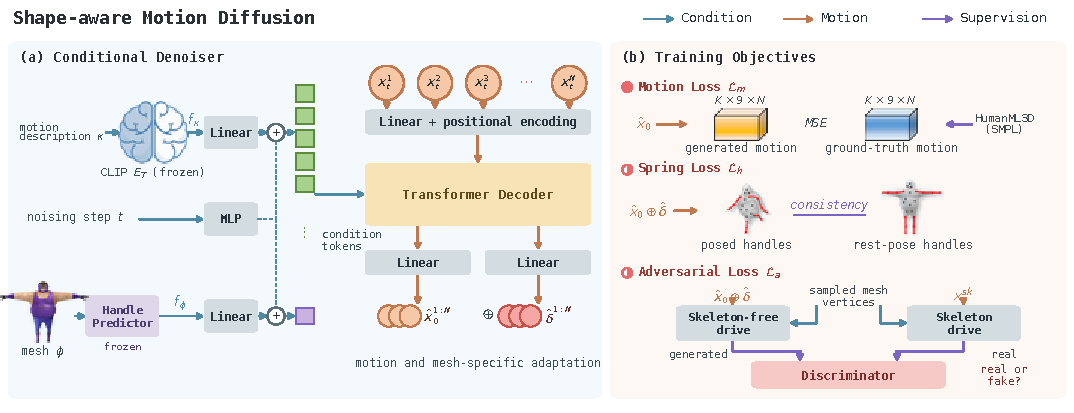
\includegraphics[width=\textwidth]{figure/method_diffusion.pdf}
  \caption{\textbf{The structure and the training strategy of Shape-aware Motion Diffusion.} The Motion Diffusion learns to generate shape-aware motions based on the textual descriptions, as well as the mesh deformation features with only the ground-truth text-motion data of the SMPL model. The parameters of the Handle Predictor are frozen during the second stage to provide stable mesh deformation features. $\bm{x}^{sk}$ is a random motion sequence in skeletal representation.}
  \label{fig:diffusion}
\end{figure*}

\textbf{Adaptive Handle Learning}. The existing 3D character datasets \blu{ModelsResource-RigNet\cite{xu2019predicting} and Mixamo\cite{mixamo}} lack handle annotations, and the skinning weights are defined independently for each character, which lacks consistency. Therefore, these datasets cannot be directly used as ground-truth. To overcome this limitation, we introduce three losses, \textit{i.e.}, Skinning Loss $\mathcal{L}_s$, Pose Loss $\mathcal{L}_p$, and Root Loss $\mathcal{L}_r$ to achieve an adaptive handle learning. Among them, the Skinning Loss $\mathcal{L}_s$ and Pose Loss $\mathcal{L}_p$ stem from \cite{liao2022skeleton}.

Following \cite{liao2022skeleton}, the assumption of $\mathcal{L}_s$ is that if two mesh vertices belong to the same body part based on the ground-truth skinning weight, they should also be assigned to the same handle by the predicted field. All three losses are imposed on the assignment $\tilde{\bm{s}}$ of Eq.~\ref{Eq.field} rather than on the deformation weights $\bm{s}$ of Eq.~\ref{Eq.rbf}, since it is the assignment that determines where the handles are placed. We select mesh vertices with $\tilde{s}_{i,k}>0.9, \exists k$ and use the KL divergence to enforce similarity between the assignments of these two vertices:
\begin{equation} \label{Eq.sup1}
\mathcal{L}_s = \gamma_{i,j} \sum_{k=1}^{K} \left( \tilde{s}_{i,k}\log(\tilde{s}_{i,k})-  \tilde{s}_{i,k}\log(\tilde{s}_{j,k})\right),
\end{equation}
where $i$ and $j$ indicate two randomly sampled vertices. $\gamma$ is an indicator function defined as follows: $\gamma_{i,j}=1$ if $i$ and $j$ belong to the same part in the ground-truth skinning weight and $\gamma_{i,j}=-1$ if not.

Pose Loss $\mathcal{L}_p$ is to ensure that the posed mesh driven by the predicted handle and skinning weight can be as similar as possible to the shape of the mesh driven by the ground-truth skeleton, which helps the predicted handle more in line with the character's articulation structure. To achieve this, we randomly select a skeletal pose for the character and drive the mesh using its skeleton to obtain a posed mesh $\bar{\bm{V}}^{p}$. Then, the local translation and local rotation of our representation can be analytically calculated according to the rest-pose mesh and the posed mesh \cite{besl1992method}. Next, we apply the local motion to the mesh using Eq.\ref{Eq.4} without the global items to obtain a skeleton-free posed mesh $\hat{\bm{V}}^{p}$. The $\mathcal{L}_p$ can be calculated by:
\begin{equation} \label{Eq.sup2}
\mathcal{L}_p = \lVert \hat{\bm{V}}^{p} - \bar{\bm{V}}^{p} \rVert_{2}^{2}.
\end{equation}

Root Loss $\mathcal{L}_r$ is to enforce the first handle point close to the character's center hip, which is an important step in animation for controlling the global motion independently. \cite{liao2022skeleton} do not take into account the global motion of the character and thus produce severe mesh distortion when applied to drive complex motions. We observe that in the traditional skeleton rigging system, the first joint of the character is always located in the hip part, which is also considered the root joint of the character. Thus, we use $\mathcal{L}_r$ to make the predicted position of the first handle $\bm{h}_{1}$ close to the position of the root joint $\bm{b}_{1}$ in the character. Substituting the first moment of Eq.~\ref{Eq.moment} for $k=1$, $\mathcal{L}_r$ is formulated as:
\begin{equation} \label{Eq.6}
\begin{aligned}
\mathcal{L}_r & = \lVert \bm{h}_{1} - \bm{b}_{1} \rVert_{2}^{2} \\ & = \Bigg\lVert \frac{\sum_{i=1}^{V}\tilde{s}_{i,1}\bar{\bm{V}}_i}{\sum_{i=1}^{V}\tilde{s}_{i,1}} - \bm{b}_{1} \Bigg\rVert_{2}^{2}.
\end{aligned}
\end{equation}
Note that this expression is well defined precisely because the root channel exists in the
assignment field: $\tilde{s}_{i,1}$ is produced by the assignment head for every vertex,
whereas the deformation weights of Eq.~\ref{Eq.rbf} are defined only for $k \geq 2$.

With the three losses introduced above, the Handle Predictor can be trained by:
\begin{equation} \label{Eq.8}
\min_{\bm{\theta}_\lambda}~\mathcal{L}_{s} + \nu_{p}\mathcal{L}_{p} + \nu_{r}\mathcal{L}_{r},
\end{equation}
where $\nu_{r}$ and $\nu_{p}$ are the loss balancing factor.

\subsection{Shape-aware Motion Diffusion} \label{sec:motion}
\blu{This module is supervised from two sources: full supervision from HumanML3D motions
converted into the handle representation of Sec.~}\ref{sec:field}, \blu{whose Handle Predictor is frozen to
provide the mesh deformation feature, and weak supervision for characters that have no
ground-truth motion.} 
The Mesh Handle Predictor enables control of heterogeneous characters through a unified motion representation, as defined in Eq.\ref{Eq.4}. This shared representation facilitates consistent motion control across characters with varying skeletal structures and topologies. However, when this representation is directly used to synthesize animations, it often results in noticeable mesh distortions. This is primarily due to the large variations in body shapes and proportions among different characters, which the unified representation alone cannot fully account for.

To address this limitation, the Shape-aware Motion Diffusion module is introduced. In addition to predicting handle motions, it also generates mesh-specific adaptation parameters that tailor the motion to each character’s unique geometry. This shape-aware adjustment significantly improves the animation quality by maintaining geometric consistency and preventing artifacts, thereby ensuring that the synthesized motions remain natural and visually plausible across diverse character models. As a result, this method is able to preserve the geometric integrity of the animations.

The left part of Figure \ref{fig:diffusion} illustrates the structure of the Shape-aware Motion Diffusion. The model takes the noising step $t$, the motion description feature $\bm{f}_{\kappa}$, and the mesh deformation feature $\bm{f}_{\phi}$ as conditions while the $t$-step noised motion $\bm{x}_{t}$ as input to generate the text-guided motion $\hat{\bm{x}}_{0}^{1:N}$ of $N$ frames and the mesh-specific adaptation $\hat{\bm{\delta}}^{1:N}$ that are suitable for the mesh $\phi$. This process is defined in Eq.\blu{\ref{Eq.3}}. For brevity, and when there is no danger of confusion, we omit the superscripts.

We \blu{employ a} Transformer Decoder \cite{vaswani2017attention} to build the denoiser of the Diffusion Model and use two linear layers to project the output features into motion and adaptation, respectively. Unlike MDM \cite{tevet2022human}, which uses a single text token from the last layer of CLIP, we utilize multiple text tokens from the penultimate layer, matching the number of words in the input motion prompt. We observe that motion distortion mainly arises from the generated local translations in our motion representation. Therefore, adaptations are applied only to the local translations, and the dimension of the motion adaptation per frame is accordingly ${(K-1) \times 3}$, matching $\bm{\tau}^{l}$. The final local translations are obtained by summing the generated local translations with the mesh-specific adaptations.

To train the Diffusion Model, we fully utilize the existing motion-language dataset \blu{HumanML3D} \cite{guo2022generating} by converting SMPL motions to our handle-based motion representation using the analytical method introduced in \cite{besl1992method} as the ground-truth motion $\bm{x}_0$. Originating from the simple loss of DDPM \cite{ho2020denoising}, a fully-supervised Motion Loss $\mathcal{L}_m$ is formulated as:
\begin{equation} \label{Eq.9}
\mathcal{L}_{m} := \mathbb{E}_{\bm{x}_0, t, \bm{f}_{\kappa}, \bm{f}_{\phi}} \left[ \lVert \bm{x}_0 - \hat{\bm{x}}_{0} \rVert^{2}_{2} \right ],
\end{equation}
where the motion $\hat{\bm{x}}_{0}$ iis generated as Eq.\blu{\ref{Eq.3}} according to the conditions $t$, $\bm{f}_{\kappa}$ and $\bm{f}_{\phi}$.

\textbf{Mesh-specific Motion Learning}. Existing motion-language datasets are primarily designed for human motions represented by the SMPL model, which limits their applicability for learning shape-aware motions across heterogeneous character meshes. To overcome this limitation, we introduce a strategy that randomly samples characters from diverse 3D character datasets \blu{(ModelsResource-RigNet\cite{xu2019predicting} and Mixamo\cite{mixamo})} during training, thereby exposing the model to a wide variety of mesh topologies.

To enable the model to capture mesh-specific information, we adopt a weakly-supervised learning paradigm. Specifically, we leverage mesh deformation features extracted by the Mesh Handle Predictor as implicit cues for mesh-aware motion adaptation. As illustrated in the right part of Figure \ref{fig:diffusion}, our approach incorporates not only a fully-supervised Motion Loss $\mathcal{L}_m$, but also two additional weakly-supervised objectives: a Spring Loss $\mathcal{L}_h$, which encourages structural consistency across deformations, and an Adversarial Loss $\mathcal{L}_a$, which promotes realistic and mesh-compatible motion patterns. Together, these losses guide the model toward effective mesh-specific motion learning, even in the absence of dense supervision for every mesh type.

The traditional skeletal rigging system of 3D characters has an important property: the length of the bones typically remains consistent during motion. This property ensures that the character's body structure remains stable throughout the animation. Drawing inspiration from this property, we propose the Spring Loss $\mathcal{L}_h$. We model the handles on the character's limbs as a spring system and penalize the length deformation of this system. Specifically, we pre-define the common adjacency relationships between the handles of the character's limbs and use the distance between adjacent handles in the rest-pose as a reference to penalize the distance changes during the character's motion:
\begin{equation} \label{Eq.10}
\begin{aligned}
\mathcal{L}_{h} = &~\sum_{i,j \in \mathcal{A}}\sum_{n=1}^{N} \Big ( e^{-\left(\mathcal{E}(h_{i}^{0},h_{j}^{0}) + \sigma \right)} \lVert \mathcal{E}(h_{i}^{n},h_{j}^{n}) -  \mathcal{E}(h_{i}^{0},h_{j}^{0}) \rVert_{2}^{2} ~+ \\ 
&~\lVert \mathcal{E}(h_{i}^{n},h_{j}^{n}) - \mathcal{E}(h_{i}^{n-1},h_{j}^{n-1}) \rVert_{2}^{2} \Big ),
\end{aligned}
\end{equation}
where $\mathcal{E}(\cdot)$ is the Euclidean Distance Function and $\sigma$ is a hyper-parameter. $i$ and $j$ are the indices of the adjacent handles. $h^{0}$ is the handle position of the rest-pose, $h^{n}$ is that of the $n$-frame pose. $e^{-\left(\mathcal{E}(h_{i}^{0},h_{j}^{0}) + \sigma \right)}$ is an adaptive spring coefficient.

The Adversarial Loss $\mathcal{L}_a$, inspired by GANs \cite{goodfellow2020generative}, is employed to encourage the generated mesh motion to align with the prior of skeleton-driven mesh motion across various characters. To reduce computational cost, we randomly sample 100 mesh vertices on the arms in each frame to compute $\mathcal{L}_a$, based on the observation that motion distortion predominantly occurs in the arms during movement. A discriminator is used to distinguish between the generated handle-driven mesh motions and the skeleton-driven ones. $\mathcal{L}_a$ is formulated following the adversarial training paradigm.
\begin{equation} \label{Eq.11}
\begin{aligned}
\mathcal{L}_{a} = &~\mathbb{E}_{\bar{V}\sim p(\bar{V}^{sk})}\big[\log Disc(\bar{V})\big]~+ \\
&~\mathbb{E}_{\bar{V} \sim p(\bar{V}^{g})}\big[\log\big(1-Disc(\bar{V})\big)\big],
\end{aligned}
\end{equation}
in which $p(\cdot)$ represents the distribution of the skeleton-driven $\bar{V}^{sk}$ or generated $\bar{V}^{g}$ mesh motions.

With the three losses introduced above, the Shape-aware Motion Diffusion can be trained by:
\begin{equation} \label{Eq.12}
% \setlength{\abovedisplayskip}{-2pt}
\setlength{\belowdisplayskip}{-1pt}
\min_{\bm{\theta}_\mu}~\mathcal{L}_{m}+ \nu_{h}\mathcal{L}_{h} + \nu_{a}\mathcal{L}_{a},
\end{equation}
where $\nu_{h}$ and $\nu_{a}$ are the balancing factors. $\mathcal{L}_{h}$ and $\mathcal{L}_{a}$ are conducted on the motion adaptation $\hat{\bm{\delta}}$.

\textbf{Motion Adaptation Fine-tuning}. To further improve the compatibility of the generated motion across heterogeneous characters and reduce mesh distortion introduced during motion transfer, we employ pseudo-labels to finetune the linear mapping layer within the motion adaptation module. These pseudo-labels are derived by optimizing the motion adaptation using an as-rigid-as-possible (ARAP) objective, which encourages local rigidity and preserves the character's structural integrity during deformation:
\begin{equation} \label{Eq.13}
\mathcal{O} = \nu_{v}\sum_{i,j \in \Phi} \lVert \mathcal{E}(\bar{V}^{n}_{i}, \bar{V}^{n}_{j}) - \mathcal{E}(\bar{V}^{0}_{i}, \bar{V}^{0}_{j}) \rVert^{2}_{2} + \lVert \bm{\delta}^{'} - \hat{\bm{\delta}} \rVert^{2}_{2}.
\end{equation}

Here, $\Phi$ represents the set of edges on the mesh, and $\bm{\delta}^{'}$ represents the optimized motion adaptation at the previous step. $\nu_{v}$ is the balancing factor.

The linear mapping layer of the motion adaptation is then finetuned by:
\begin{equation} \label{Eq.14}
% \setlength{\abovedisplayskip}{-2pt}
\setlength{\belowdisplayskip}{-1pt}
\min_{\bm{\theta}_{\mu}^{\delta}}~\lVert \bm{\delta}^{pl} - \hat{\bm{\delta}} \rVert^{2}_{2},
\end{equation}
where $\bm{\delta}^{pl}$ is the pseudo-labels of the motion adaptations, $\bm{\theta}_{\mu}^{\delta}$ is the learnable parameters.


\subsection{Unified Objective} \label{sec:unified}
The three modules above are trained under a single objective,
\begin{equation} \label{Eq.unified}
\begin{aligned}
\min_{\Theta,\bm{\psi},\bm{\theta}_{\mu}}\ \
& \mathcal{L}^{\text{rest}}_{\text{diff}}
+\lambda_{1}\mathcal{L}_{\text{pose}}
+\lambda_{2}\mathcal{R}_{\text{anim}} \\
+\ & \lambda_{3}\big(\mathcal{L}_{s}+\nu_{p}\mathcal{L}_{p}+\nu_{r}\mathcal{L}_{r}\big)
+\lambda_{4}\big(\mathcal{L}_{m}+\nu_{h}\mathcal{L}_{h}+\nu_{a}\mathcal{L}_{a}\big),
\end{aligned}
\end{equation}
where the first line collects the terms of the Pose-aware Mesh Generator, the third group
those of the handle field and the fourth group those of the Shape-aware Motion Diffusion.
Optimisation proceeds in three stages for tractability --- the field and the motion model are
trained first, then frozen while $\Theta$ is optimised per character, and finally the field is
fine-tuned jointly --- but the objective being optimised is one.

It is worth making explicit what Eq.~\ref{Eq.unified} changes with respect to a cascade of a
generator followed by an animator. In a cascade the joint density factorises as
$p_{\varphi}(\phi\mid m,I)\,p_{\lambda}(\mathcal{H}\mid\phi)\,p_{\mu}(\bm{x}\mid
\bm{f}_{\phi},\bm{f}_{\kappa})$, in which the first factor contains neither $\mathcal{H}$ nor
$\kappa$. The generator gradient then reduces to $\nabla_{\Theta}\mathcal{L}_{\text{total}}=
\nabla_{\Theta}\mathcal{L}^{\text{rest}}_{\text{diff}}$ and, equivalently,
\begin{equation} \label{Eq.mixed}
\frac{\partial^{2}\mathcal{L}_{\text{total}}}
{\partial\Theta\,\partial\bm{\theta}_{\mu}}=\bm{0},
\end{equation}
so the optimum of the generator is independent of the animator and the two components are
separable in the strict sense: either could be replaced without affecting the other. The two
coupling terms $\mathcal{L}_{\text{pose}}$ and $\mathcal{R}_{\text{anim}}$ both depend on
$\Theta$ through $\mathcal{D}$ and on $\bm{\theta}_{\mu}$ through the sampled motion, hence
under Eq.~\ref{Eq.unified} the mixed second derivative of Eq.~\ref{Eq.mixed} no longer
vanishes. Sec.~\ref{sec:exp} measures this non-separability directly, by estimating the
interaction between the two stages in a factorial design instead of asserting it.

\begin{figure*}[t]
\centering
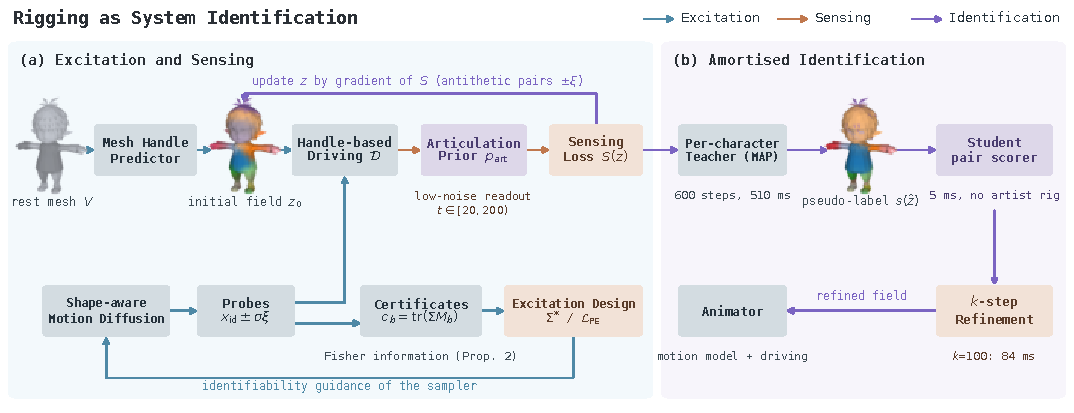
\includegraphics[width=\textwidth]{figure/sysid_overview.pdf}
\caption{\rev{\textbf{Rigging as system identification.} (a) The motion model excites the field:
probes $\bm{x}_{\text{id}}\pm\sigma\bm{\xi}$ drive the rest mesh through the handle-based operator, the
articulation prior scores the driven points at low noise, and the gradient of the sensing loss of
Eq.~\ref{Eq.sense} updates the assignment. The per-boundary certificates of Eq.~\ref{Eq.Ib} set the
excitation design of Eq.~\ref{Eq.sdp} and Eq.~\ref{Eq.lpe}, which also guides the sampler
(Eq.~\ref{Eq.guide}). (b) Per-character identification (Eq.~\ref{Eq.teacher}) supplies pseudo-labels
for a feed-forward student, whose output is refined by $k$ steps of the same objective before driving.
The renders show a RigNet test character coloured by handle.}}
\label{fig:sysid_overview}
\end{figure*}

\begin{revblock}
\subsection{Rigging as System Identification} \label{sec:sysid}
The coupling terms above guarantee that the generative gradient reaches the handle field. This
subsection asks how much \textit{information} that gradient carries, and answers it with the
tools of system identification: the field is the unknown, the motion is the excitation, and the
prior that scores the deformed asset is the sensor. Fig.~\ref{fig:sysid_overview} summarises the
resulting pipeline.

\textbf{Setting.} Let $\bm{z}$ collect the parameters of the assignment, i.e.\ the field
$\mathcal{H}_{\bm{\psi}}$ evaluated at the points, and $\bm{s}(\bm{z})$ the resulting weights. A
sensor observes the driven asset, $\bm{y}=\mathcal{O}\big(\mathcal{D}(\bm{V};\bm{x},\bm{s}(\bm{z}))\big)
+\bm{n}$ with precision $\bm{P}$, under probing motions
$\bm{x}=\bm{x}_{\text{id}}+\sigma\bm{\xi}$, $\mathbb{E}[\bm{\xi}]=\bm{0}$,
$\mathrm{Cov}[\bm{\xi}]=\bm{\Sigma}$.

\textbf{Proposition 1 (the rest pose carries no information).} At the identity motion every
summand of Eq.~\ref{Eq.4} is the identity and the weights sum to one, so
$\mathcal{D}(\bm{V};\bm{x}_{\text{id}},\bm{s})=\bm{V}$ for every $\bm{s}$. Hence
$\partial\bm{y}/\partial\bm{z}=\bm{0}$, $\nabla_{\bm{z}}\mathcal{L}^{\text{rest}}=\bm{0}$, and the
Fisher information of any rest-pose observation about $\bm{z}$ vanishes identically. This is the
information-theoretic content of Eq.~\ref{Eq.gauge}: the field is not identifiable from
appearance, under any prior.

\textbf{Proposition 2 (information is linear in the probe covariance).} To first order,
$\mathcal{D}(\bm{V};\bm{x}_{\text{id}}+\sigma\bm{\xi},\bm{s})=\bm{V}+\sigma\bm{G}_{\bm{z}}\bm{\xi}
+O(\sigma^{2})$, where the columns $\bm{g}_{a}(\bm{z})$ of $\bm{G}_{\bm{z}}$ are the displacements
produced by the elementary handle motions. The Fisher information about $\bm{z}$ is then
\begin{equation} \label{Eq.fisherlin}
\mathcal{I}_{q}(\bm{z})=\sigma^{2}\sum_{a,b}\Sigma_{ab}\,
\big(\partial_{\bm{z}}\bm{g}_{a}\big)^{\!\top}\bm{P}\,\big(\partial_{\bm{z}}\bm{g}_{b}\big)
\;=\;\sigma^{2}\mathcal{A}_{\bm{z}}(\bm{\Sigma}),
\end{equation}
a linear map of $\bm{\Sigma}$. Since $\partial\mathcal{D}/\partial s_{k}-\partial\mathcal{D}/
\partial s_{l}=\bm{u}_{k}(\bm{p})-\bm{u}_{l}(\bm{p})$ with
$\bm{u}_{k}(\bm{p})=\bm{R}^{l}_{k}(\bm{p}-\bm{h}_{k})+\bm{\tau}^{l}_{k}+\bm{h}_{k}-\bm{p}$, the
information about the boundary $b=(k,l)$ between two adjacent handles is
\begin{equation} \label{Eq.Ib}
I_{b}(\bm{\Sigma})=\mathrm{tr}\big(\bm{\Sigma}\,\bm{M}_{b}\big),\qquad \bm{M}_{b}\succeq\bm{0},
\end{equation}
where $\bm{M}_{b}$ accumulates the relative displacement of handles $k$ and $l$ over the
points of the boundary band. A boundary is informative only when the two handles that share it
move relative to each other.
\end{revblock}

\begin{revblock}
\textbf{Proposition 3 (persistent excitation).} $\bm{z}$ is locally identifiable, up to the gauge
of Eq.~\ref{Eq.gauge}, if and only if $\mathcal{A}_{\bm{z}}(\bm{\Sigma})$ is non-singular on the
non-gauge directions \cite{rothenberg1971identification}, which by the block structure of
Eq.~\ref{Eq.Ib} holds if and only if $I_{b}(\bm{\Sigma})>0$ for every boundary $b$, i.e.\ if every
pair of adjacent handles is moved relative to each other by the probes. This is the
skinning counterpart of persistent excitation \cite{ljung1999system}, and it explains
uniformly why existing rigging methods work: each of them obtains the excitation from outside
the character, through example poses, video, or artist rigs.

\textbf{Certificate.} Proposition~2 turns the information into a per-boundary quantity that is
computed before any identification is run. By the Cram\'er--Rao bound the variance of any
unbiased estimate of the boundary is at least the corresponding diagonal entry of
$\mathcal{I}_{q}^{-1}$, so $c_{b}=I_{b}(\bm{\Sigma})$ ranks boundaries by how well the probes
can determine them. A boundary that the motion distribution never excites receives
$c_{b}\approx0$ and is flagged as unidentified rather than silently guessed.

\textbf{Excitation design.} Because Eq.~\ref{Eq.fisherlin} is linear in $\bm{\Sigma}$, choosing
the probes that best determine the weakest boundary is a semidefinite programme,
\begin{equation} \label{Eq.sdp}
\begin{aligned}
\bm{\Sigma}^{\star}=\arg\max_{\bm{\Sigma}\succeq\bm{0}}\ &\min_{b}\ \mathrm{tr}(\bm{\Sigma}\bm{M}_{b})\\
\text{s.t.}\ \ &\mathrm{tr}\,\bm{\Sigma}=\mathrm{tr}\,\bm{\Sigma}_{\mu},\ \
\bm{\Sigma}\preceq\kappa\bm{\Sigma}_{\mu},
\end{aligned}
\end{equation}
the E-optimal design of \cite{kiefer1960equivalence} restricted to the motions that the
motion prior, with covariance $\bm{\Sigma}_{\mu}$, deems plausible. For a model that generates the
probes itself we use the amortised, smooth form
\begin{equation} \label{Eq.lpe}
\begin{aligned}
\mathcal{L}_{\text{PE}}(\hat{\bm{\Sigma}})={}&-\operatorname{softmin}_{b}\ \log I_{b}(\hat{\bm{\Sigma}})\\
&+\lambda\,\mathrm{KL}\big(\mathcal{N}(\bm{0},\hat{\bm{\Sigma}})\,\big\|\,\mathcal{N}(\bm{0},\bm{\Sigma}_{\mu})\big),
\end{aligned}
\end{equation}
where $\hat{\bm{\Sigma}}$ is the covariance of the generated probes and $\lambda$ trades
identifiability against fidelity to the motion prior. Sec.~\ref{sec:exp_id} shows that the
soft-min matters: with full covariances the max--min design of Eq.~\ref{Eq.sdp} lowers the worst
boundary on human characters at a small cost in average error, but restricted to per-joint
variances it concentrates the budget on a few joints and raises both errors, whereas the
amortised form of Eq.~\ref{Eq.lpe} lowers both.
\end{revblock}

\begin{revblock}
\subsection{Second-order Prior Sensing} \label{sec:sensor}
Propositions~1--3 hold for any sensor with precision $\bm{P}$. When no observation of the
moving character exists, the only available sensor is a frozen generative prior, which scores
how plausible the driven asset is. Writing $\ell(\bm{x},\bm{z})=\log p\big(\mathcal{O}(
\mathcal{D}(\bm{V};\bm{x},\bm{s}(\bm{z})))\big)$, the rest term is independent of $\bm{z}$ by
Proposition~1 and the first-order term averages out, so
\begin{equation} \label{Eq.second}
\mathbb{E}_{\bm{\xi}}\big[\ell(\bm{x}_{\text{id}}+\sigma\bm{\xi},\bm{z})\big]=
\ell(\bm{x}_{\text{id}})+\tfrac{\sigma^{2}}{2}\,\mathbb{E}_{\bm{\xi}}\big[\bm{\xi}^{\top}
\bm{H}_{\bm{z}}\,\bm{\xi}\big]+O(\sigma^{3}):
\end{equation}
the first signal about the field is the curvature of the prior along the probing motion. By the
second-order Tweedie formula \cite{meng2021estimating,manor2024posterior} this curvature is a
projection of the posterior covariance of the denoiser, so it can be estimated with forward
passes only, without back-propagating through the denoiser. A single-sided probe, however, also
carries a zero-mean first-order term; the single-sample signal-to-noise ratio is
\begin{equation} \label{Eq.snr}
\mathrm{SNR}_{1}(\sigma)=\mathrm{SNR}_{\infty}\,\frac{\sigma}{\sqrt{\sigma^{2}+\sigma_{\ast}^{2}}},
\qquad \mathrm{SNR}_{\pm}(\sigma)\equiv\mathrm{SNR}_{\infty},
\end{equation}
where $\sigma_{\ast}$ is the ratio of the first- to the second-order fluctuation, and pairing
$\pm\bm{\xi}$ \cite{salimans2017evolution} removes the odd terms exactly. At visible probe
amplitudes the expansion of Eq.~\ref{Eq.second} is no longer accurate, so in practice we
estimate the finite-amplitude objective directly with antithetic pairs,
\begin{equation} \label{Eq.sense}
\begin{aligned}
S(\bm{z})&=\mathbb{E}_{\bm{\xi},\,t\in\mathcal{T},\,\bm{\epsilon}}\Big[\tfrac{1}{2}\sum_{\pm}
\big\lVert\hat{\bm{\epsilon}}\big(\bm{y}_{\pm},t\big)-\bm{\epsilon}\big\rVert^{2}\Big],\\
\bm{y}_{\pm}&=\mathcal{O}\big(\mathcal{D}(\bm{V};\bm{x}_{\text{id}}\pm\sigma\bm{\xi},\bm{s}(\bm{z}))\big),
\end{aligned}
\end{equation}
of which Eq.~\ref{Eq.second} is the small-$\sigma$ limit. Both ingredients are necessary: with
$\sigma=0$ the gradient of Eq.~\ref{Eq.sense} vanishes by Proposition~1, and with a flat prior it
vanishes because the denoiser carries no curvature.
\end{revblock}

\begin{revblock}
\textbf{Which prior can sense the field.} Eq.~\ref{Eq.sense} is only useful if the prior ranks
deformations by where they bend rather than by how much they move. We tested every prior family
available to us on the same controlled task (Sec.~\ref{sec:exp_id}): rendered-image priors
\cite{rombach2022high}, a pose detector \cite{yang2023dwpose}, vision--language models
\cite{qwen3vl2025} and a video diffusion model \cite{wan2025wan}. None of them reliably locates a
joint along a limb, and the diffusion priors among them are dominated by the overall magnitude of
the deformation and prefer the candidate that moves the least, which is the failure mode of
likelihoods reported in \cite{nalisnick2019deep}. We therefore use
an \textit{articulation prior} that observes the deformation directly in 3D: a diffusion model
over point displacements conditioned on the rest surface,
\begin{equation} \label{Eq.artprior}
p_{\text{art}}\big(\bm{d}\mid\bm{P}\big),\qquad
\bm{d}=\mathcal{D}(\bm{P};\bm{x},\bm{s})-\bm{P},
\end{equation}
where $\bm{P}$ are $1{,}024$ points sampled on the rest surface. Its training data are generated
on the fly from static 3D data only, without any 4D mesh sequence; motion capture enters only as
a distribution of single poses. They are the training split of RigNet and
Mixamo posed with their own skinning weights under random sparse or dense joint rotations and
Mixamo motion capture, and SMPL-H bodies \cite{loper2015smpl} with random shapes in the static
poses of HumanML3D \cite{guo2022generating}. The denoiser is a 22M-parameter transformer over
point tokens with a cosine noise schedule. Because the observation is the deformed geometry
itself, no renderer or image autoencoder sits between the probe and the prior, which is the
setting in which Eq.~\ref{Eq.snr} was verified.

\textbf{Low-noise readout.} The denoising loss at high noise levels depends almost only on the
global magnitude of $\bm{d}$, and on our benchmark it is \textit{anti}-correlated with the correct
partition; the local structure that distinguishes a correct boundary is resolved only at low
noise. We therefore restrict $\mathcal{T}$ in Eq.~\ref{Eq.sense} to $t\in[20,200)$ of $1{,}000$
steps. A likelihood ratio against a background model trained on skeleton-agnostic soft-part
motions \cite{ren2019likelihood}, the standard correction for this bias, performed worse than
the low-noise readout in all our tests and is not used.

\textbf{What the sensor determines.} The articulation prior identifies the \textit{partition} of
the field --- which vertices move with which handle --- reliably, also on the non-human test
characters. It does not reliably determine where a boundary lies along a limb segment:
none of the priors we tested, 2D or 3D, locates a joint along the bone much better than chance.
In the pipeline the
sensor therefore adjudicates the assignment between handles, and the position of a boundary
within a segment is left to the geometric bandwidth term of Eq.~\ref{Eq.rbf}. The certificate of
Proposition~2 measures the excitation, not the sensor: computed with the precision of an exact
sensor, it does not reveal this blindness of the prior. The sensing
objective acts on $\bm{\psi}$ only and enters Eq.~\ref{Eq.unified} as an additional term
$\lambda_{5}S(\bm{z}(\bm{\psi}))$.
\end{revblock}

\begin{revblock}
\subsection{Amortised Identification} \label{sec:amortise}
Identifying the field per character requires an optimisation for every new asset. We amortise
it into the Mesh Handle Predictor, so that inference returns to a single forward pass.

\textbf{Teacher.} For a character with initial assignment $\bm{z}_{0}$, obtained geometrically
from the rest shape, and probes $\{\bm{x}_{m}\}_{m=1}^{M}$ drawn from $\bm{\Sigma}^{\star}$ or from
the motion prior, the teacher solves the per-character maximum a posteriori problem
\begin{equation} \label{Eq.teacher}
\begin{aligned}
\hat{\bm{z}}=\arg\min_{\bm{z}}\ &\sum_{m=1}^{M}\big\lVert\bm{y}_{m}-\mathcal{O}\big(
\mathcal{D}(\bm{V};\bm{x}_{m},\bm{s}(\bm{z}))\big)\big\rVert^{2}_{\bm{P}}\\
&+\lambda_{z}\lVert\bm{z}-\bm{z}_{0}\rVert^{2},
\end{aligned}
\end{equation}
and returns the pseudo-label $\bm{s}(\hat{\bm{z}})$ together with the certificates $c_{b}$.

\textbf{Student.} The predictor is trained on the pseudo-labels of many characters with a soft
cross-entropy. Since characters have different numbers of active handles, the student scores
every (vertex, handle) pair from pair features and the trunk embedding, normalises the scores over
the handles of the character, and adds them as a residual to the logit of $\bm{z}_{0}$, so that it
starts from the geometric assignment. At inference, the student's output can be refined by $k$
steps of Eq.~\ref{Eq.teacher} warm-started from it; the student thereby supplies the prior and
the refinement supplies the evidence of the probes. We also tested weighting the pseudo-labels by
their certificates, which is statistically optimal if the teacher attains the Cram\'er--Rao
bound; it brought no measurable gain (Sec.~\ref{sec:exp_id}) and is not used.

\textbf{Identifiability in motion sampling.} The motion model can be asked to generate motions
that excite the field. At every denoising step of the Shape-aware Motion Diffusion the predicted
clean motion is moved along the gradient of the soft-min term of Eq.~\ref{Eq.lpe},
\begin{equation} \label{Eq.guide}
\hat{\bm{x}}_{0}\leftarrow\hat{\bm{x}}_{0}+\eta\,\frac{\bm{g}}{\lVert\bm{g}\rVert_{\text{rms}}},
\qquad
\bm{g}=\nabla_{\hat{\bm{x}}_{0}}\operatorname{softmin}_{b}\log I_{b}\big(\hat{\bm{x}}_{0}\big),
\end{equation}
where $I_{b}$ is evaluated on the boundaries of the \textit{current} field, never on ground truth,
over all frames of a batch of generated motions. The step size $\eta$ trades identifiability
against fidelity to the text-conditioned distribution, and $\eta=0$ recovers the original sampler.

\textbf{Scope of the experiments.} To separate the three questions, Sec.~\ref{sec:exp_id} evaluates
identification and amortisation with an exact sensor that observes the deformed vertices, and
evaluates the prior sensors separately on a controlled benchmark with artist rigs as ground truth.
\end{revblock}

\section{Experiments} \label{sec:exp}

\subsection{Experimental Setup}
% \begin{figure*}[h] % 强制尽量在当前位置显示
%   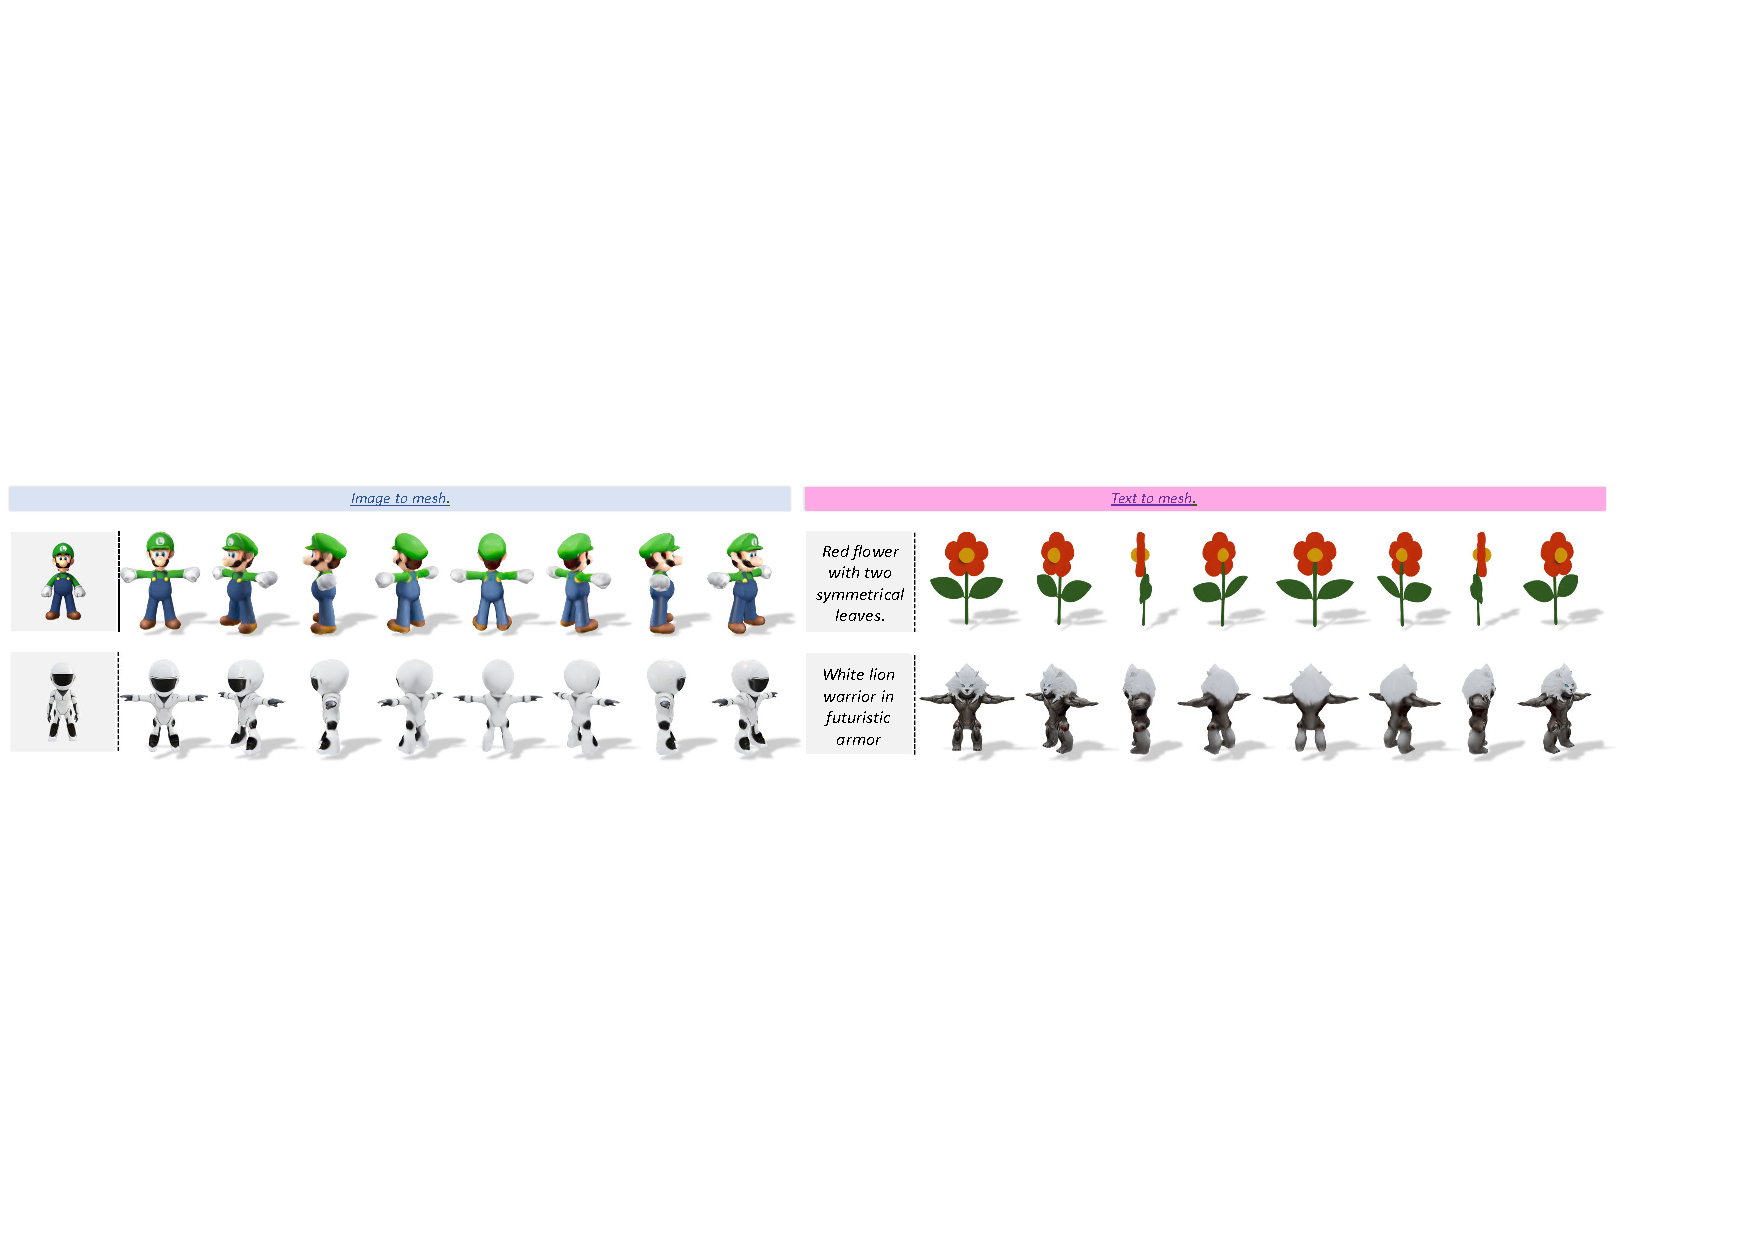
\includegraphics[width=1.0\linewidth]{figure/mesh.pdf}
%   \caption{\textbf{Visualization of the multi-view rest-pose meshes.} Overall qualitative results of the rest-pose meshes generated based on images and text.}
%   \label{fig:fig5}
% \end{figure*}

% \begin{figure*}[h] % 强制尽量在当前位置显示
%   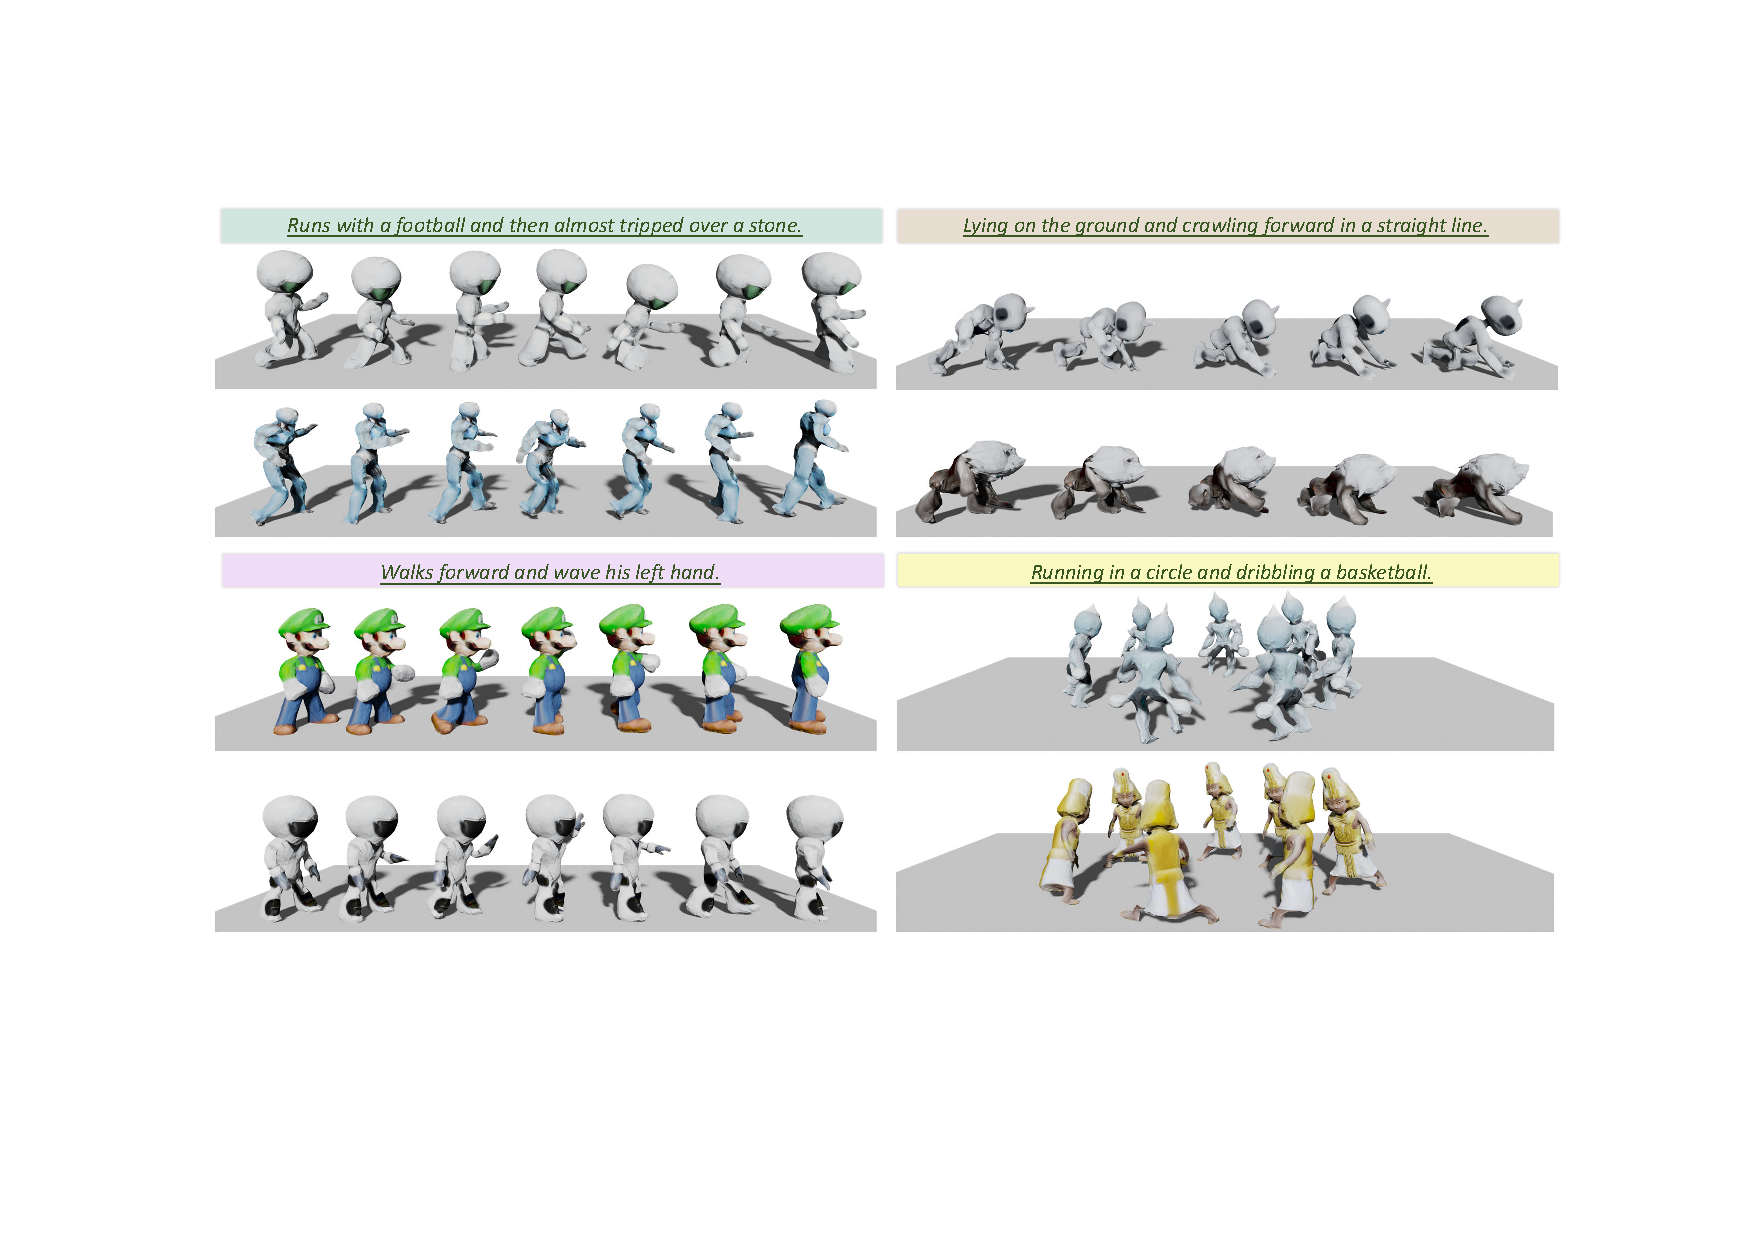
\includegraphics[width=1.0\linewidth]{figure/fig6.pdf}
%   \caption{\textbf{Visualization of the multi-view rest-pose meshes.} Overall qualitative results of the rest-pose meshes generated based on images and text.}
%   \label{fig:fig6}
% \end{figure*}
\textbf{Baselines}. To the best of our knowledge, TapMeMo is the first pipeline to generate animations for skeleton-free characters in a text-driven manner. We design two reasonable baselines to evaluate the effectiveness of our TapMeMo. 1) \textbf{MDM $+$ skeleton-based retargeting (MDM-SR).} MDM \cite{tevet2022human} is a popular motion generation method for the SMPL model. We use MDM to generate human motion based on the text, then automatically rig the skeleton template of the SMPL model to the character by \cite{baran2007automatic}, and finally retarget the human motion to the character by motion copy. 2) \textbf{MDM $+$ SfPT (MDM-SFR).} We use MDM to generate human motion, then use SfPT \cite{liao2022skeleton} to transfer the human motion to the character frame by frame.

\textbf{Datasets}. \blu{Six} public datasets are used to train and evaluate our TapMeMo, i.e., AMASS \cite{mahmood2019amass}, Mixamo \cite{mixamo}, ModelsResource-RigNet \cite{xu2019predicting},  HumanML3D \cite{guo2022generating}, \blu{Objaverse\cite{deitke2023objaverse} and AnimalML3D\cite{yang2024omnimotiongpt}.
1)} \textbf{AMASS} \cite{mahmood2019amass} is a large-scale motion dataset with over 11K sequences unified via the SMPL model, which decouples pose and shape parameters for flexible synthesis.
\blu{2)} \textbf{Mixamo} \cite{mixamo} offers diverse 3D characters and 1,112 motion sequences. We use 100 characters and retarget motions via joint correspondences for animation diversity.
\blu{3)} \textbf{RigNet} \cite{xu2019predicting} includes 2,703 rigged 3D characters with heterogeneous meshes and skeletons. We adopt the official train-test split.
\blu{4)} \textbf{HumanML3D} \cite{guo2022generating} provides 14,616 SMPL-based motion sequences with 44,970 text annotations, converted to our format via \cite{besl1992method}, following the split from \cite{guo2020action2motion}.
\blu{5)} \textbf{Objaverse} \cite{deitke2023objaverse} contains over 800,000 3D objects spanning more than 21,000 categories, with detailed object labels, textual descriptions, and animation information. From this collection, we curated a high-quality subset of approximately 70,000 objects for training and evaluation.
\blu{6) \textbf{AnimalML3D}\cite{yang2024omnimotiongpt} is a text–motion dataset for diverse animal characters, featuring motions with non-human skeletal structures.}

\textbf{Metrics}. We evaluate our TapMeMo quantitatively in terms of motion and geometry quality. For motion quality, we follow the approach in \cite{guo2022generating}, where motion representations and text descriptions are embedded using a pre-trained feature extractor and evaluated with five metrics. Since our motion representation differs from theirs, we retrain the feature extractor to align with our approach. For geometry quality, we assess it based on mesh vertices and handles using \blu{three} metrics:
1) \textbf{\blu{Self-intersection rate}}\blu{. Following Posealign and Siamotion, we report the
percentage of mesh faces that intersect another face of the same mesh, averaged over all frames of a
sequence. This is our primary geometry metric: it appears in none of our training or pseudo-label
objectives and is computed identically for every method.
2) \textbf{ARAP Error} gauges} the level of local distortion of the mesh during the characters'
motion, which can be calculated by:
\begin{equation} \label{Eq.15}
\mathcal{L}_{ARAP} = \sum_{i,j \in \Phi} \lVert \mathcal{E}(\bar{V}^{n}_{i}, \bar{V}^{n}_{j}) - \mathcal{E}(\bar{V}^{0}_{i}, \bar{V}^{0}_{j}) \rVert^{2}_{2},
\end{equation}
where $\Phi$ is the set of edges on the mesh. \blu{This quantity} is similar to the ARAP
objective in Eq.\blu{~\ref{Eq.13} without its second term; since that objective is also used to produce
the pseudo-labels of the motion adaptation, we report the ARAP Error only as a secondary reference
rather than as the primary criterion.} 3) \textbf{Handle-FID}. To assess the global
geometry quality, we employ two SMPL human models that vary significantly in body size by adjusting the shape parameters. Using FID, we measure the distribution distances between the handle positions of the generated motion and the real motion on these two models. 

The five metrics \cite{guo2022generating} for evaluating motion quality are listed as follows:
\blu{1)} R-Precision. We provide a single motion sequence and 32 text descriptions, consisting of one ground truth and 31 randomly selected mismatched descriptions. We calculate the Euclidean distances between the motion and text embeddings and rank them. We report the accuracy of motion-to-text retrieval at Top-1, Top-2, and Top-3 accuracy. \blu{2)} Frechet Inception Distance (FID). Calculating the distribution distance between the generated and real motion using FID \cite{heusel2017gans} on the extracted motion features. \blu{3)} Multimodal Distance (MM-Dist). The average Euclidean distances between each text feature and the generated motion feature corresponding to this text. \blu{4)} Diversity. We randomly select 300 motion pairs from a set, extract their features, and calculate the average Euclidean distances between the pairs to quantify motion diversity within the set. \blu{5)} Multimodality (MModality). We generate 20 motion sequences for each text description, resulting in 10 pairs of motion. For each pair, we extract motion features and calculate the average Euclidean distance between them. The reported metric is the average distance over all text descriptions.
\begin{figure*}[h]
\vspace{-.2cm}
\setlength{\abovecaptionskip}{-.5mm}
\setlength{\belowcaptionskip}{-.3cm}
  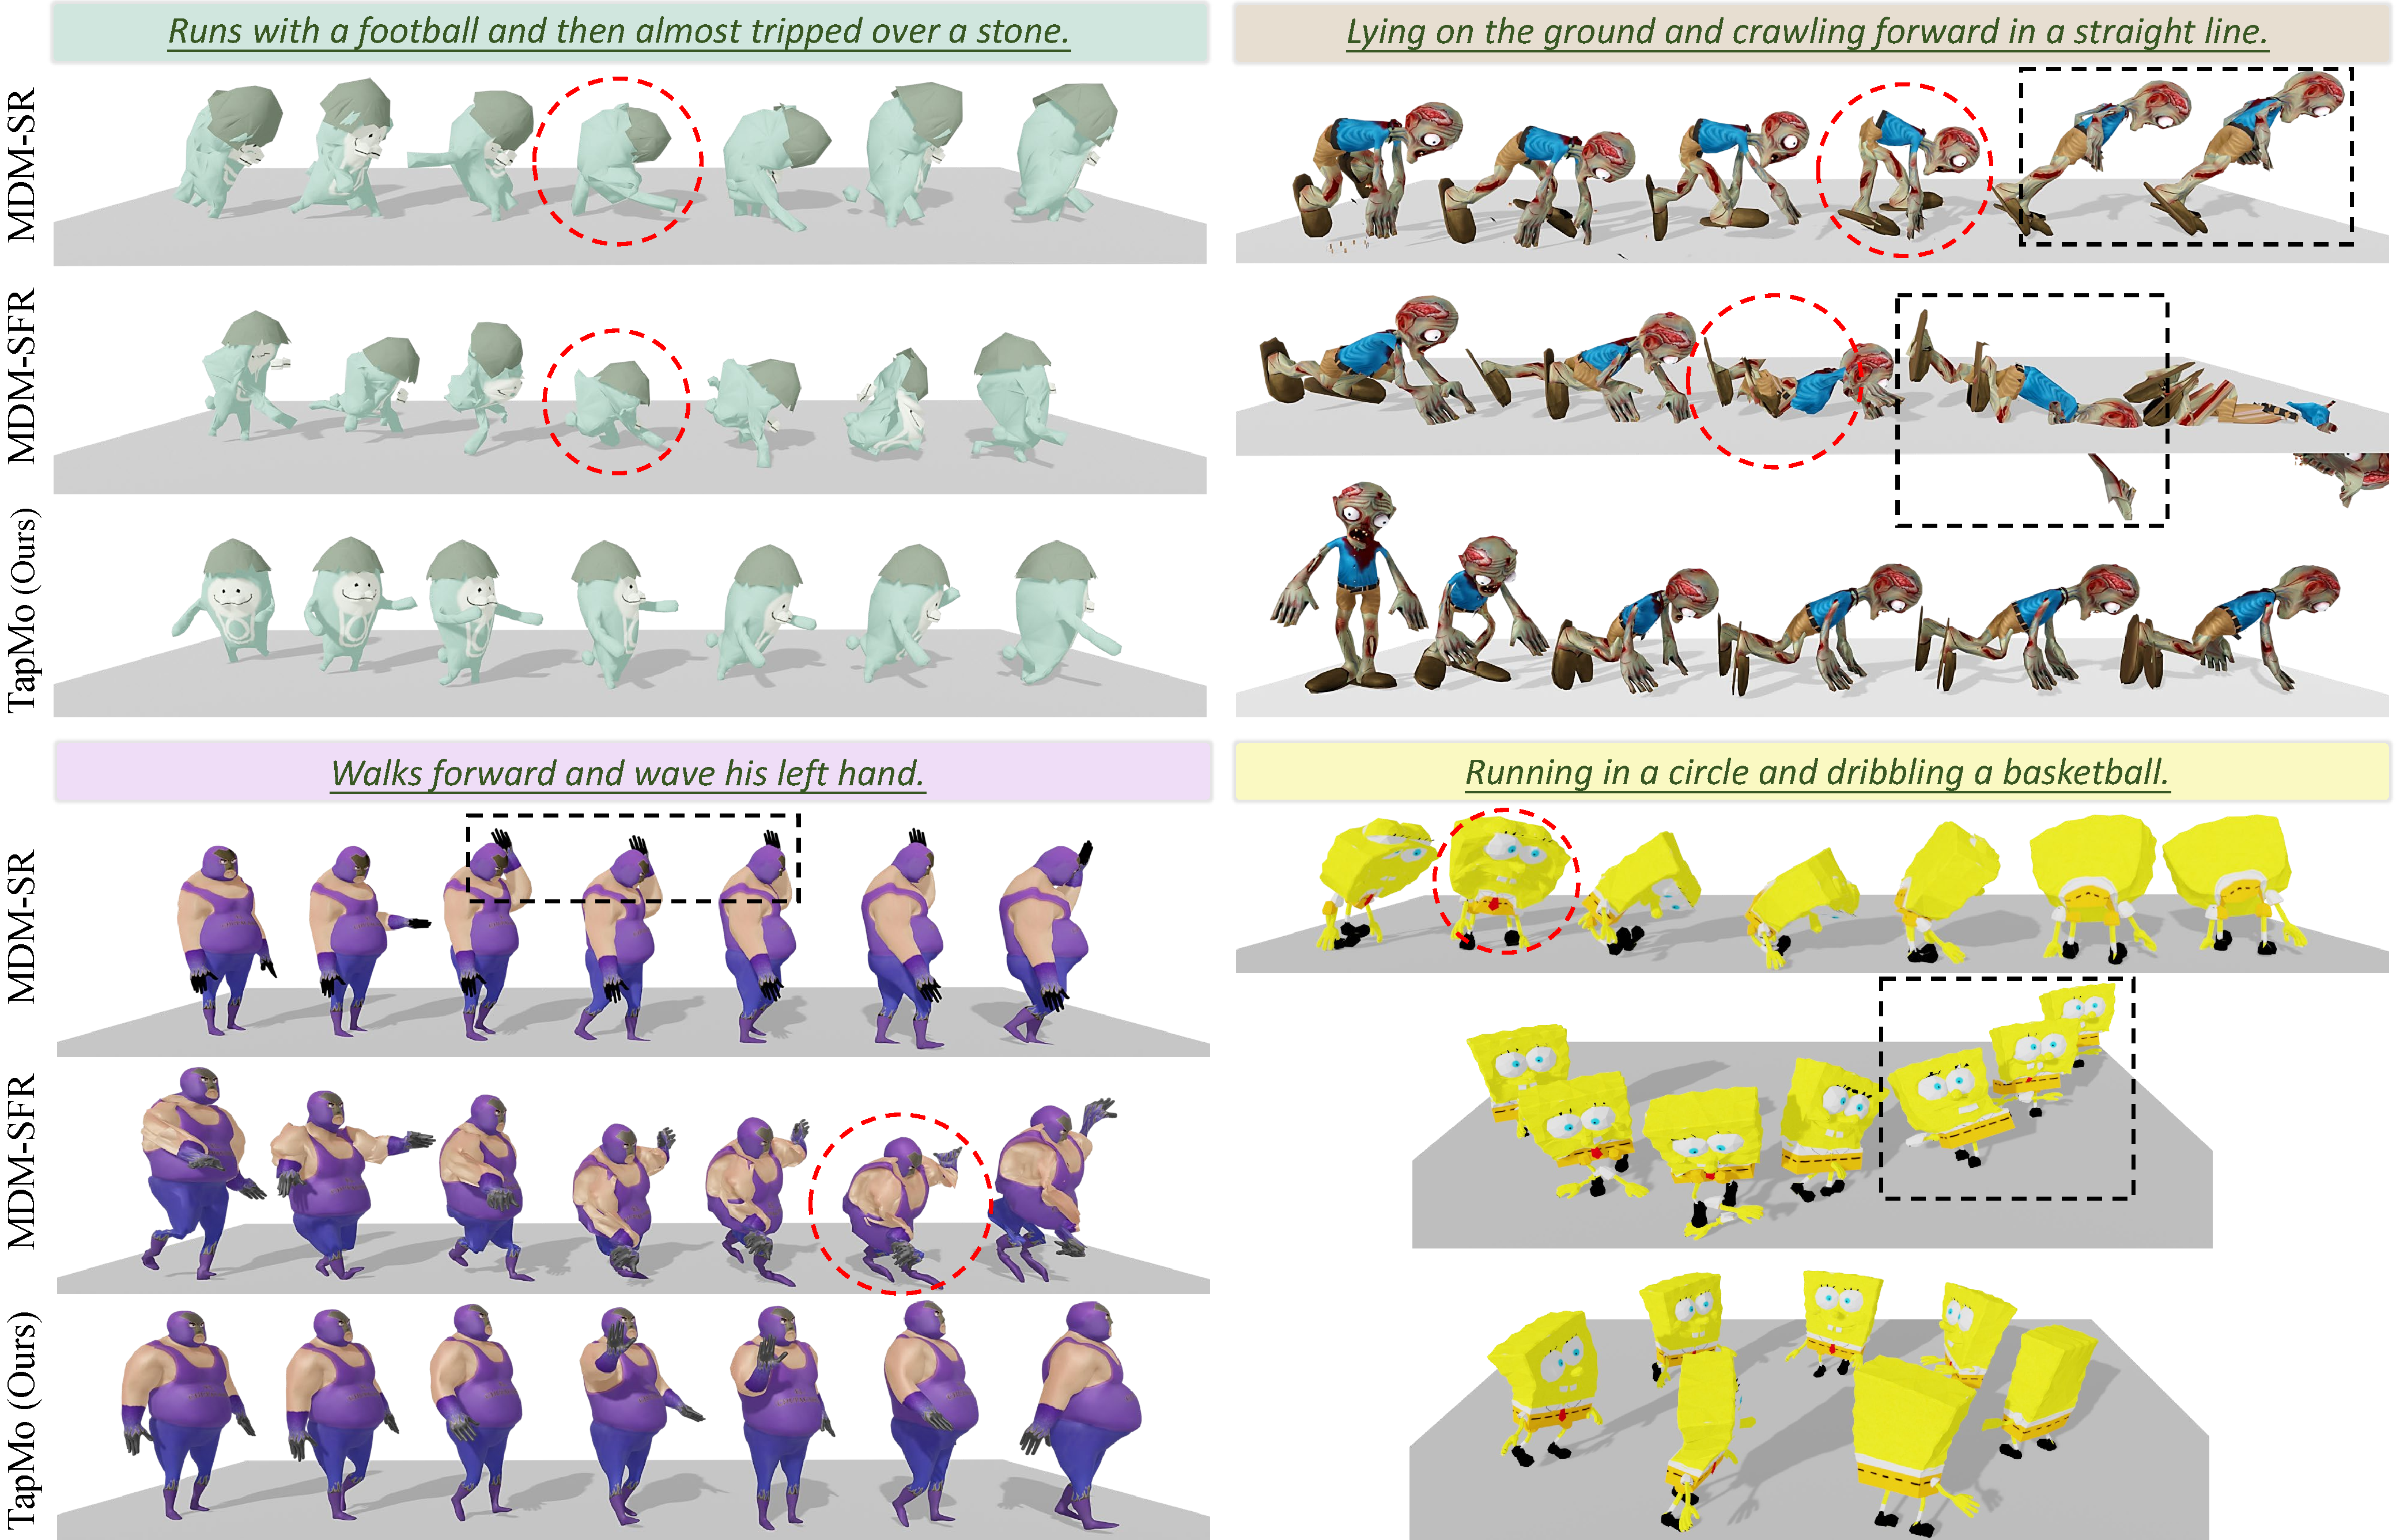
\includegraphics[width=1.0\linewidth]{figure/overallresults.pdf}
  \caption{\textbf{Qualitative comparison of the generated animations.} The red circle indicates that this sample suffers from severe mesh distortion. The black wireframe indicates that this sample does not align with the motion description.}
  \label{fig:overallresults}
\end{figure*}


\subsection{Qualitative Results}
\begin{figure*}[h]
\centering
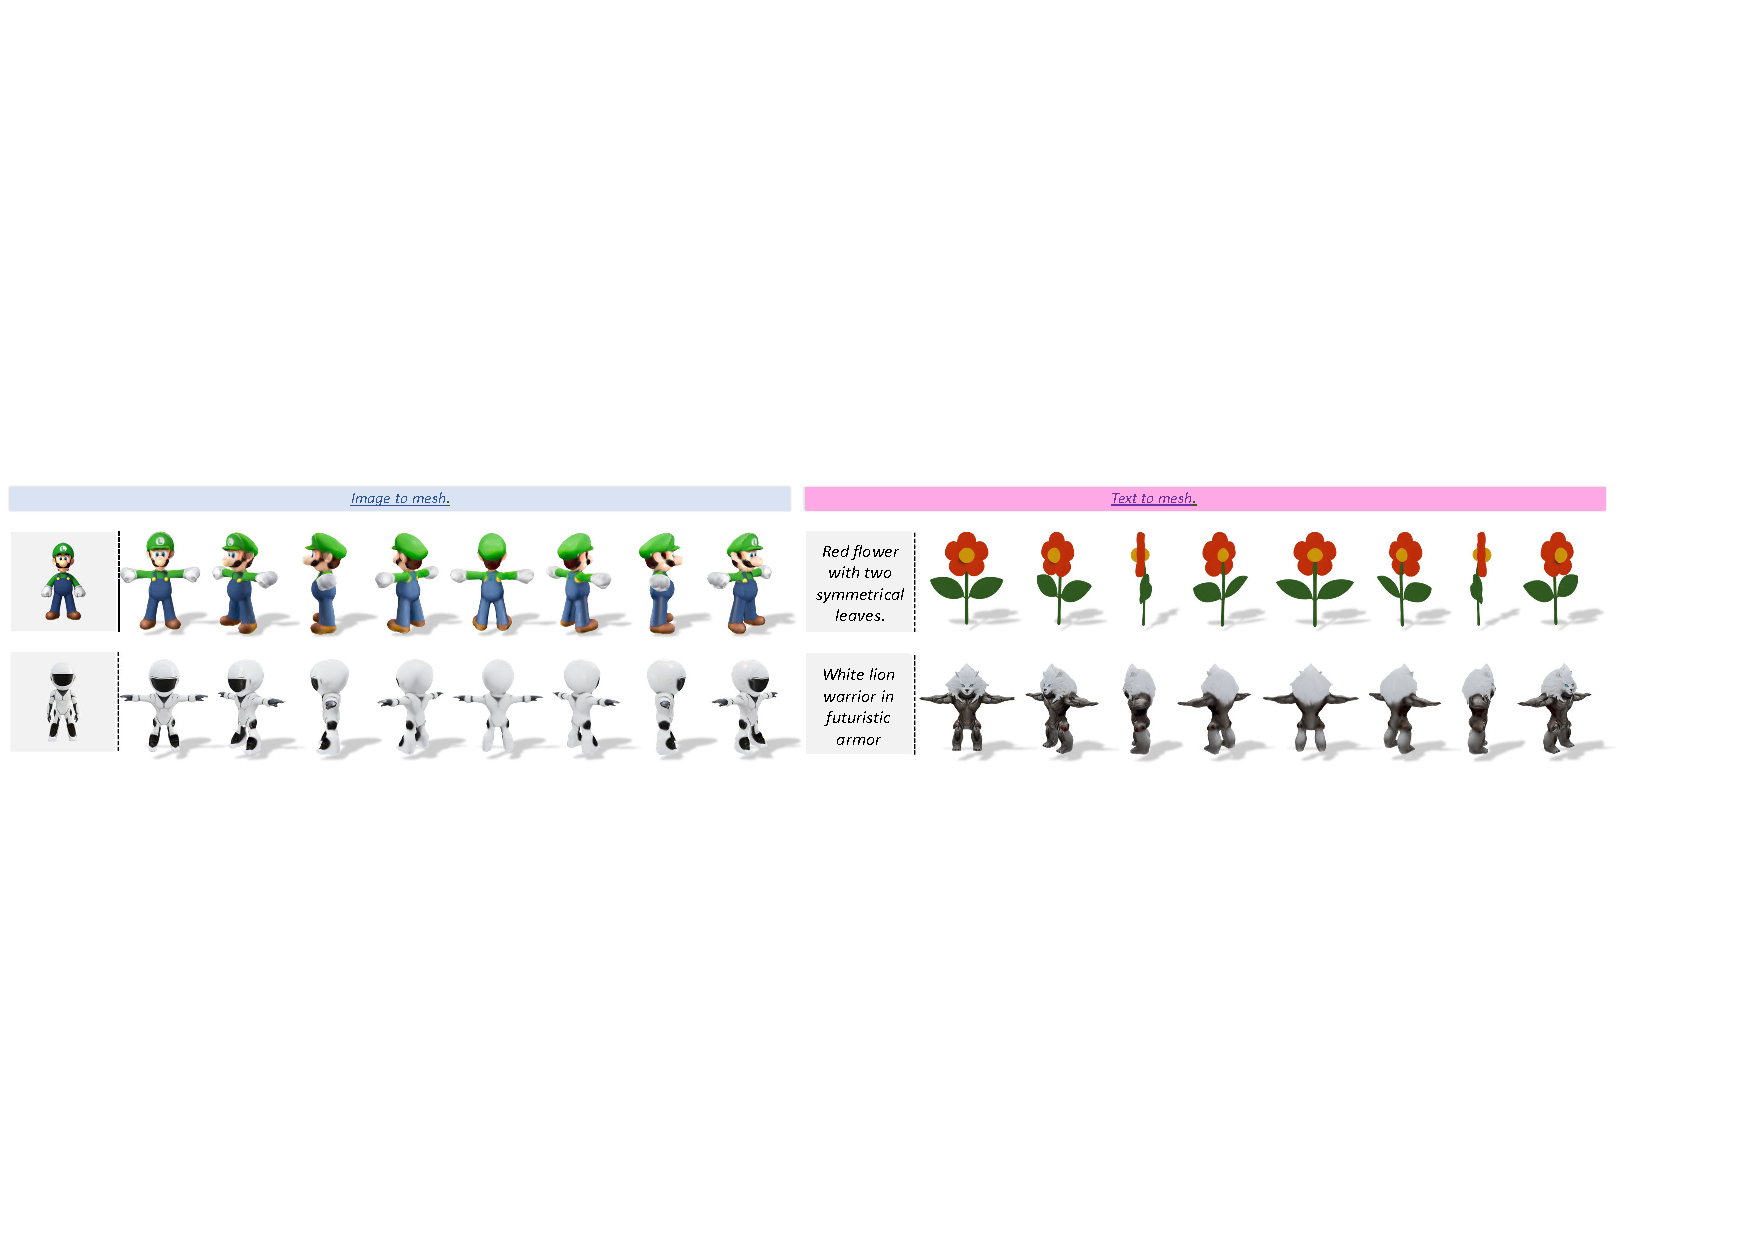
\includegraphics[width=1.0\linewidth]{figure/mesh.pdf}
\caption{\textbf{Visualization of the multi-view rest-pose meshes.} Overall qualitative results of the rest-pose meshes generated based on images and text.}
\label{fig:fig5}
\end{figure*}
\begin{figure*}[h]
\centering
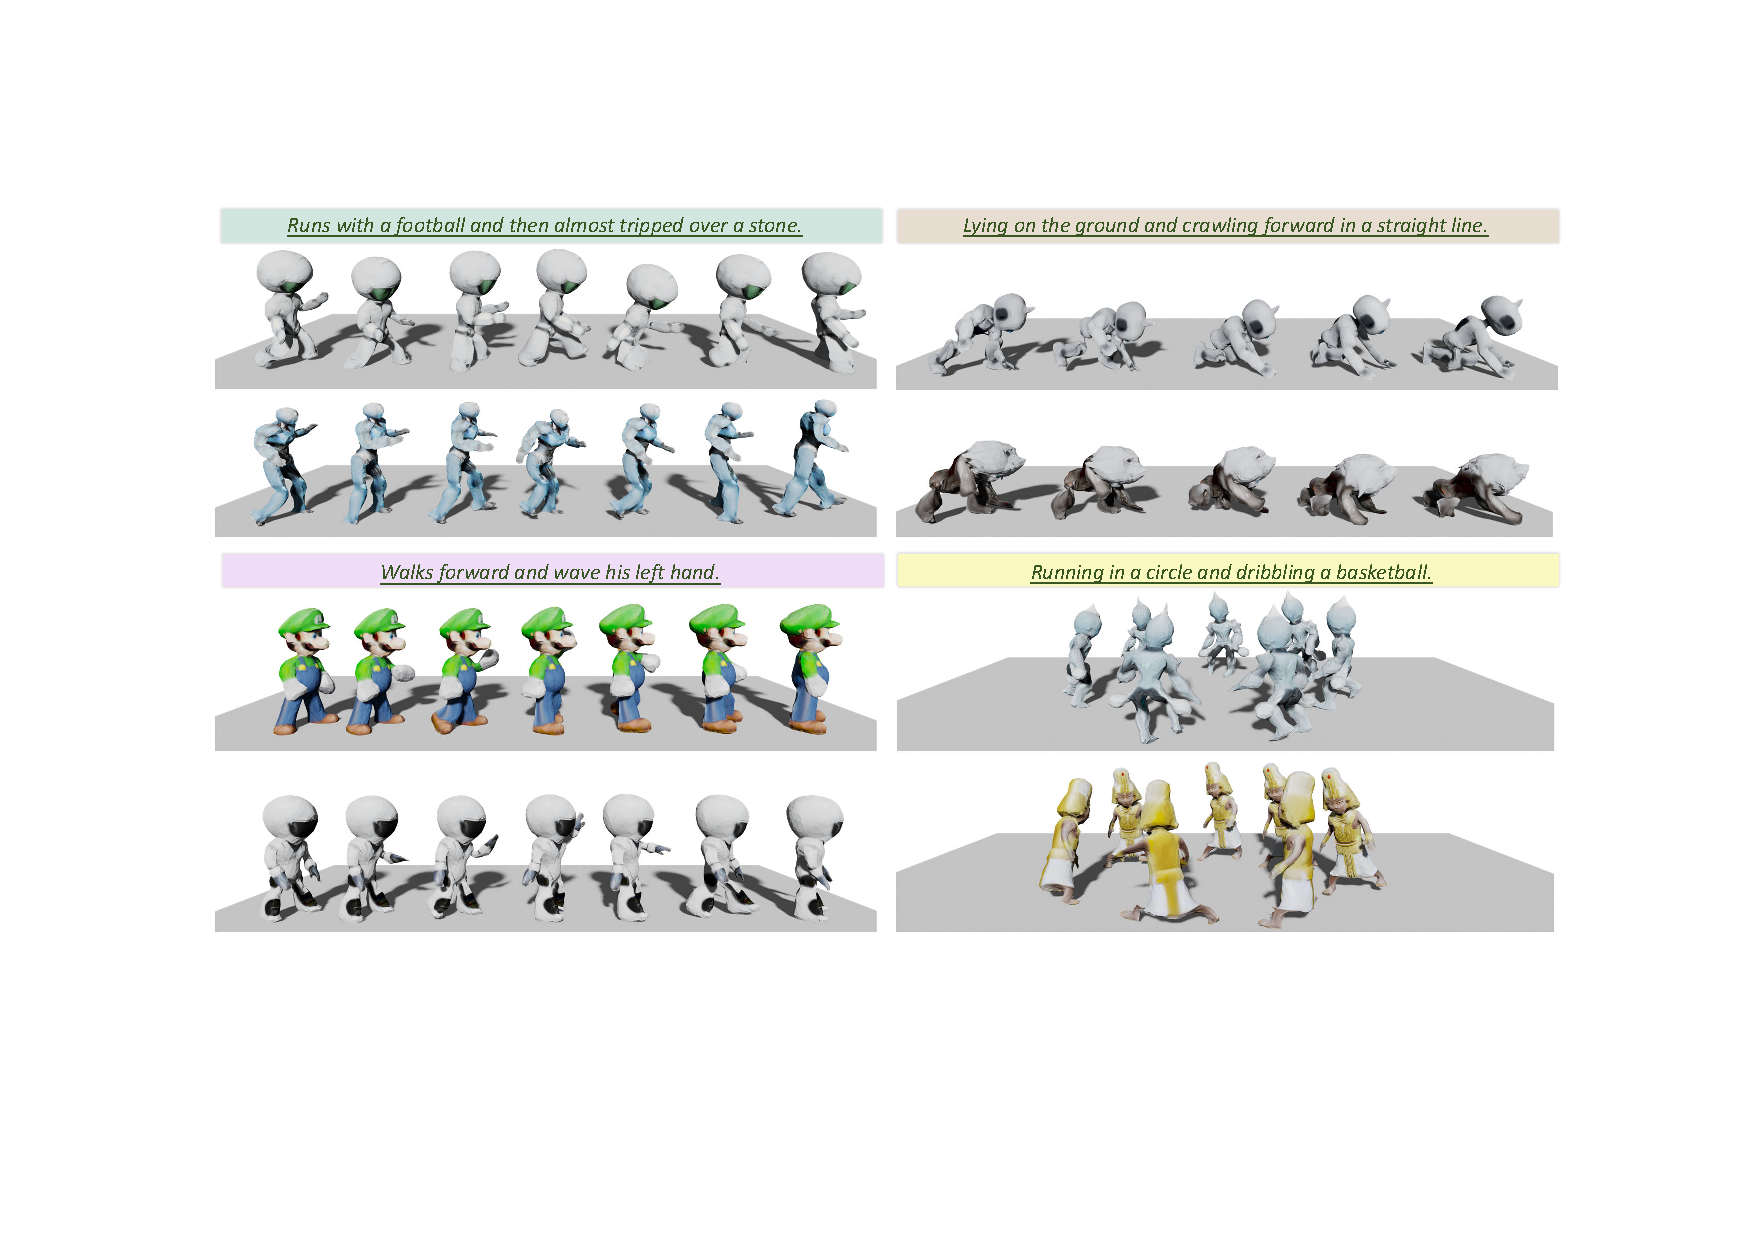
\includegraphics[width=1.0\linewidth]{figure/fig6.pdf}
\caption{\textbf{Animation driving of rest-pose meshes.} These rest-pose meshes are driven to exhibit natural and fluid motions, efficiently transforming into dynamic and expressive animations.}
\label{fig:fig6}
\end{figure*}
\begin{figure*}[h]
\vspace{-.3cm}
\setlength{\abovecaptionskip}{-.5mm}
\setlength{\belowcaptionskip}{-.3cm}
  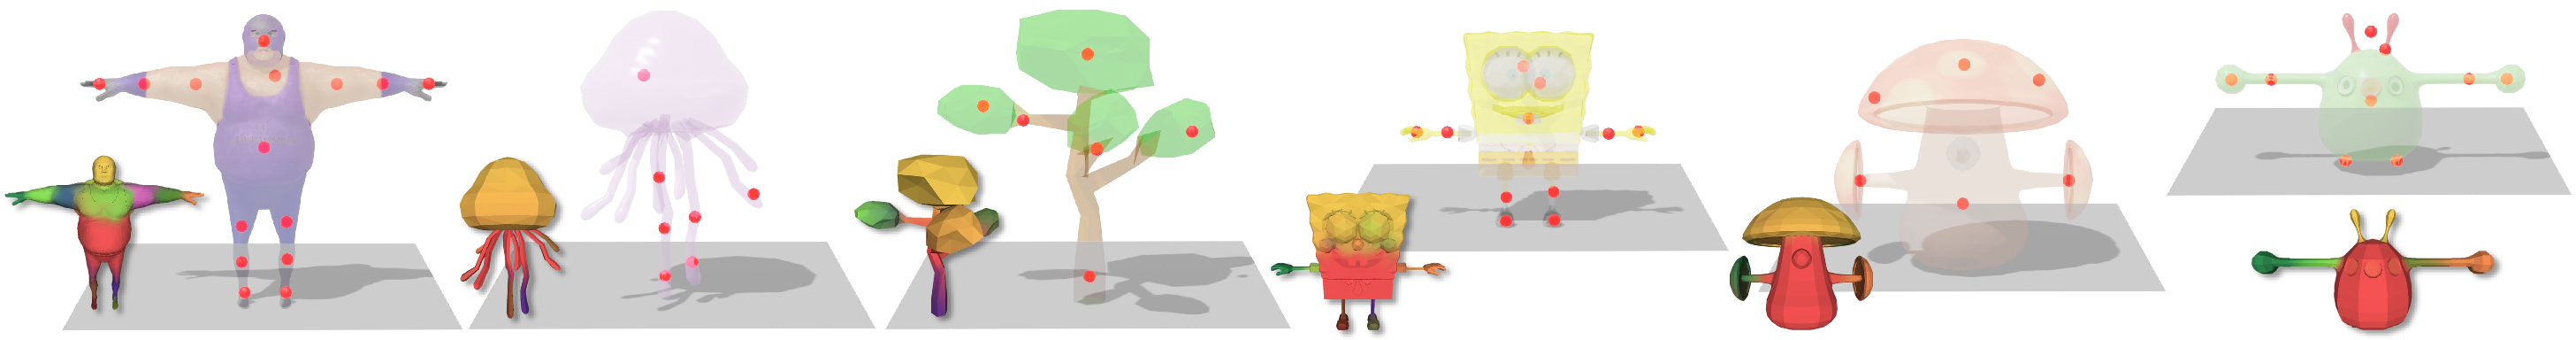
\includegraphics[width=0.95\linewidth]{figure/handles.pdf}
  \caption{\textbf{Visualization of the mesh handles and their corresponding skinning weights.} The skinning weights that correspond to the root handle are highlighted in red.}
  \label{fig:handlepos}
\end{figure*}

\begin{figure*}[h]
% \vspace{-.8cm}
\setlength{\abovecaptionskip}{-.5mm}
\setlength{\belowcaptionskip}{-.3cm}
  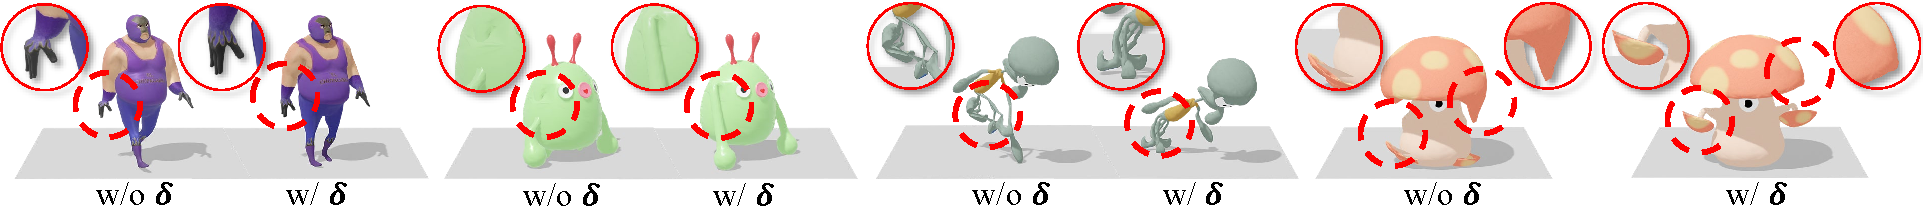
\includegraphics[width=1.0\linewidth]{figure/delta.pdf}
  \caption{\textbf{Illustration of the impact of the mesh-specific motion in TapMeMo.} ``w/ $\delta$'' and ``w/o $\delta$'' means the animation results with or without equipping the motion adaptations. The mesh-specific motion adaptations generated by TapMeMo can effectively alleviate the mesh distortion in animations.}
  \label{fig:delta}
\end{figure*}
\begin{figure*}[]
  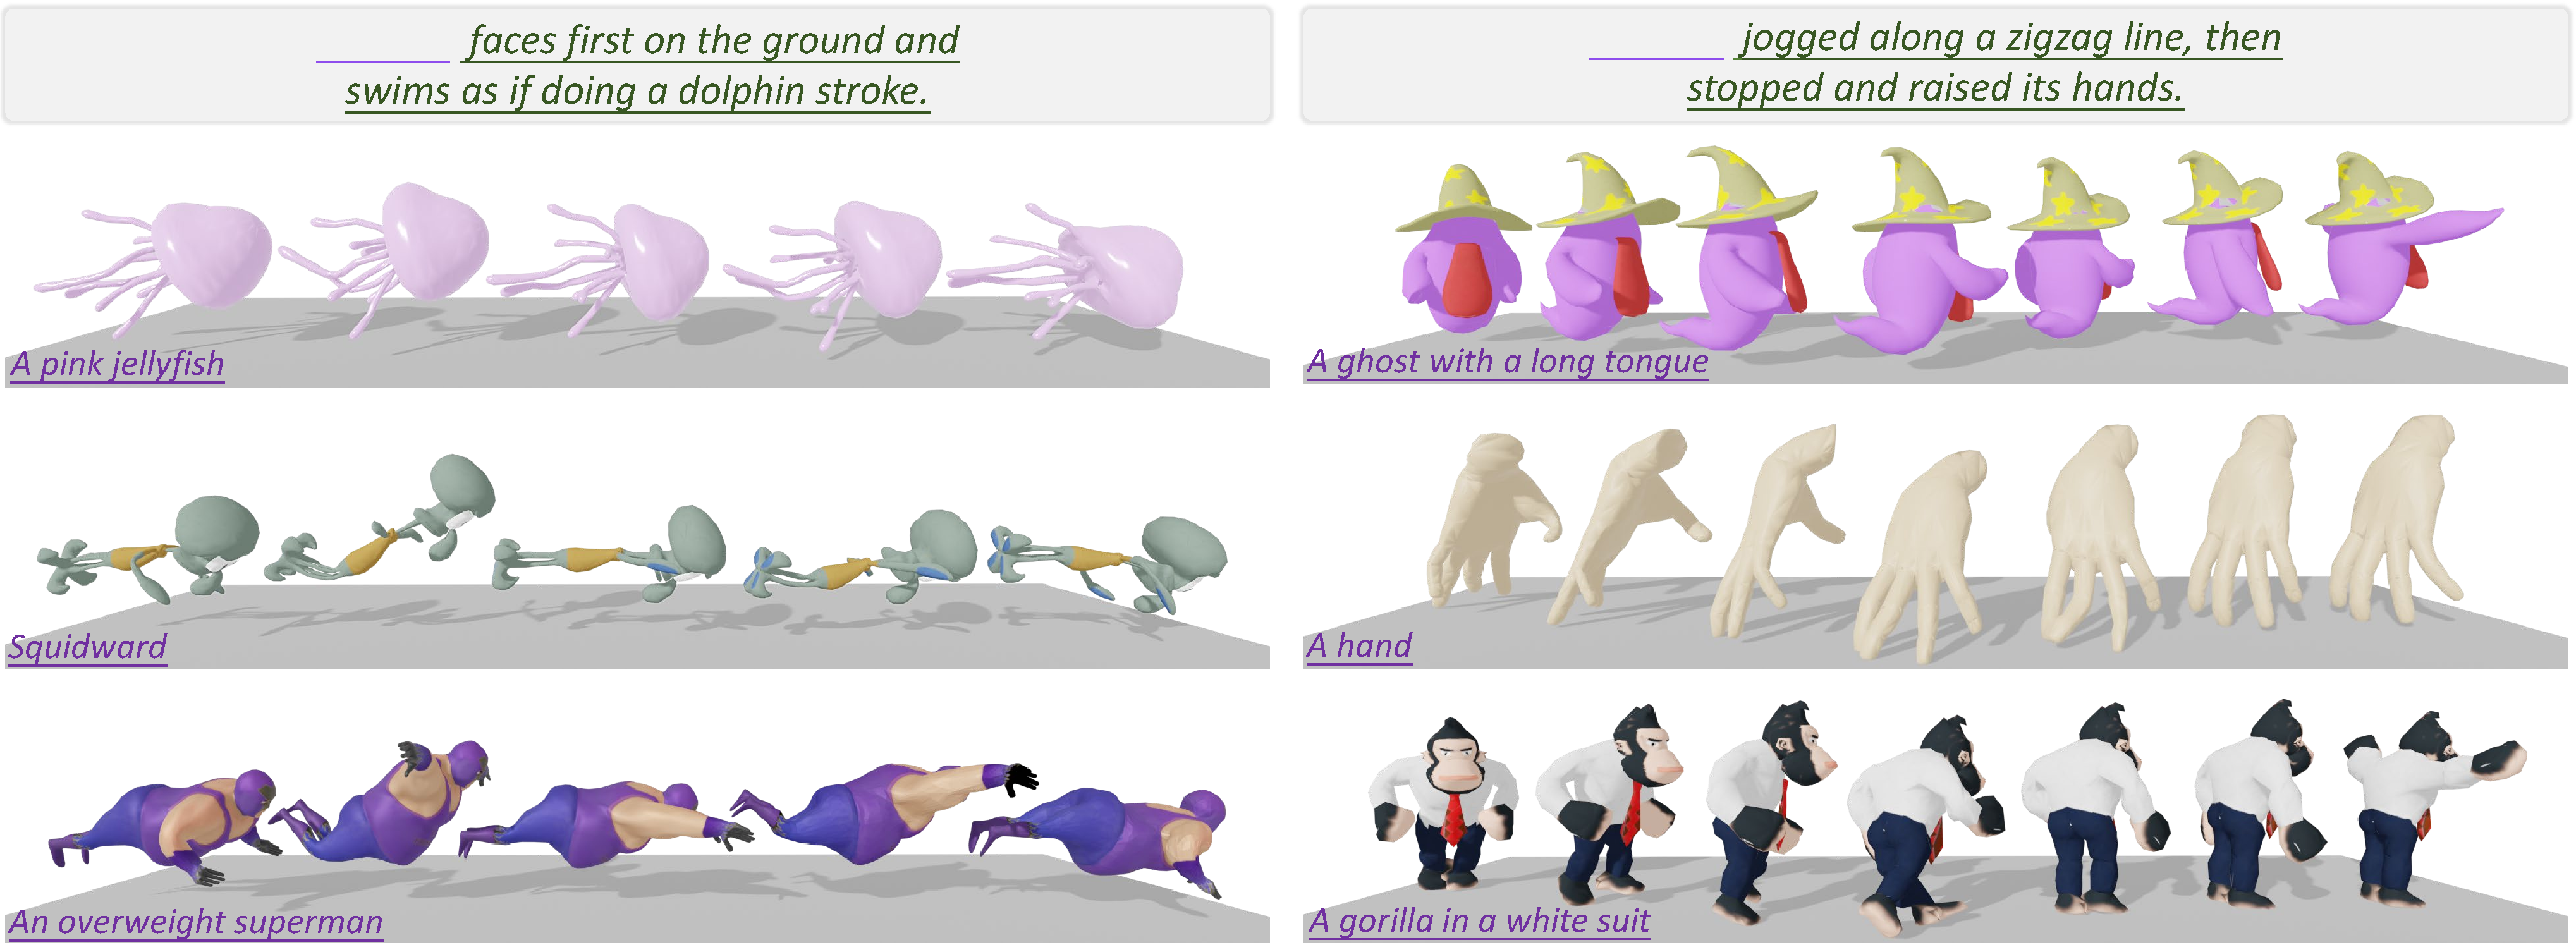
\includegraphics[width=1.0\linewidth]{figure/motionresult.pdf}
  \caption{\textbf{Qualitative results of executing the same motion descriptions with characters of different shapes.} TapMeMo can generate mesh-specific motions for characters without causing noticeable mesh distortion while utilizing adaptive handles to drive the characters naturally.}
  \label{fig:motionresult}
\end{figure*}

\begin{figure*}[]
  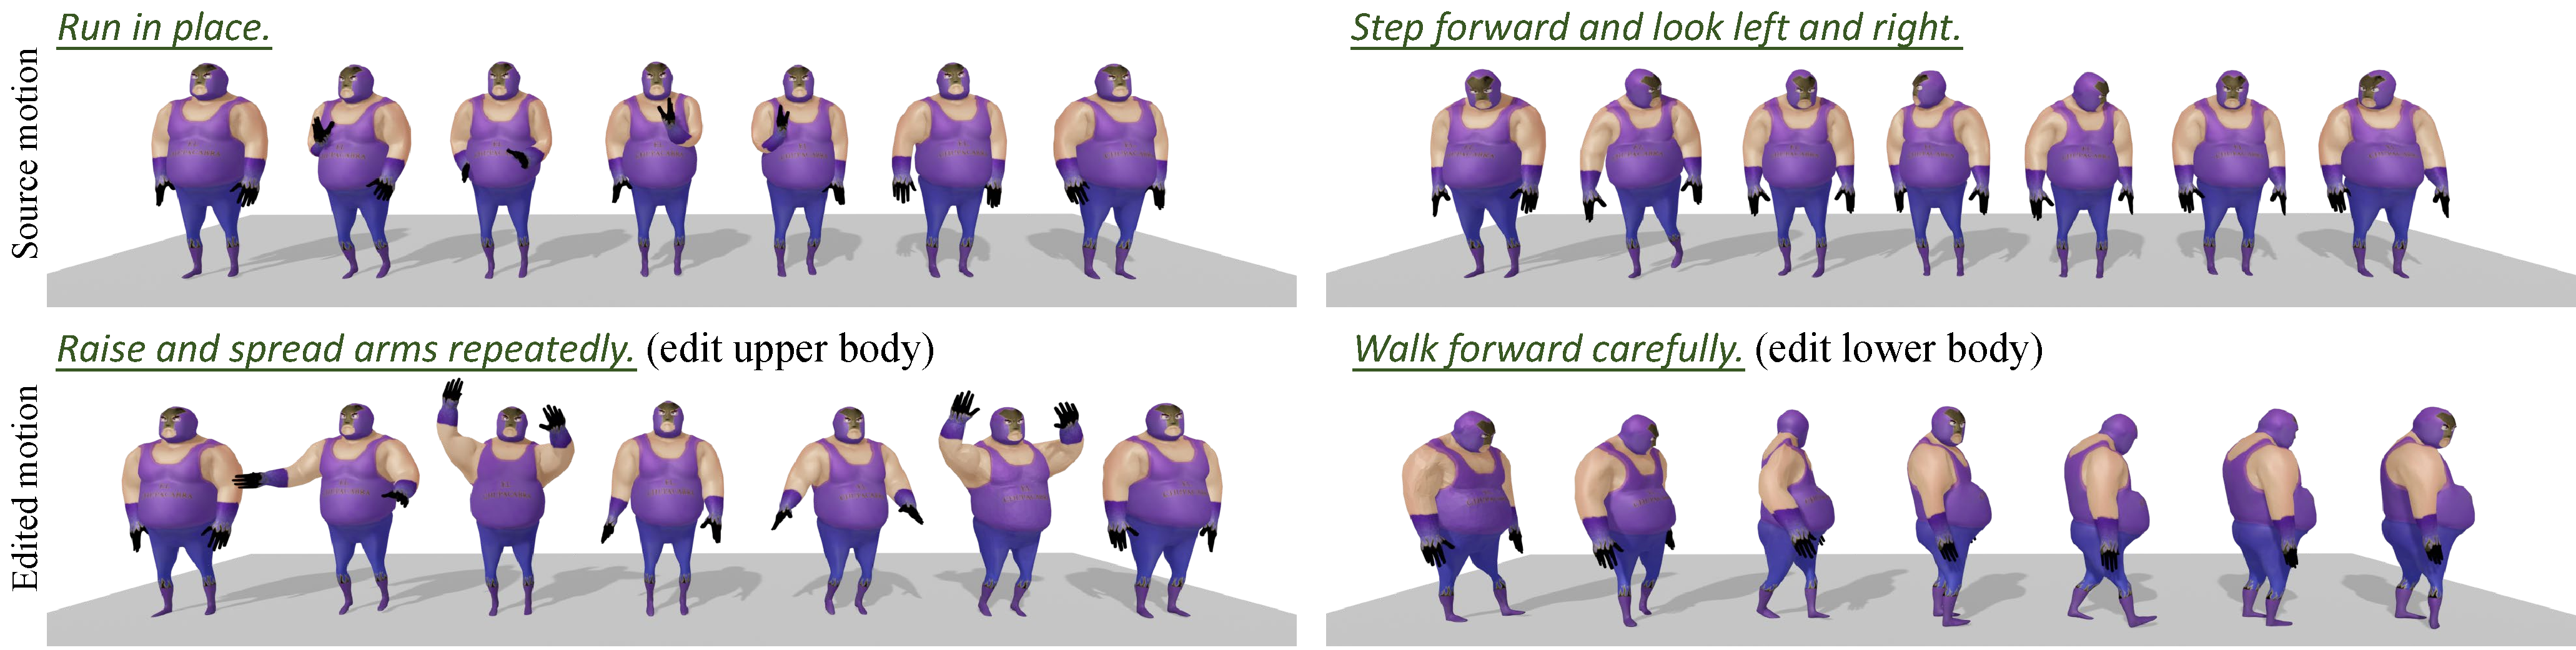
\includegraphics[width=1.0\linewidth]{figure/editing.pdf}
  \caption{\textbf{Examples of animation editing.} The left part and the right part of this figure are the generated results of editing the upper body and lower body of the character, respectively. Please note that we edit the upper body (the left one) and the lower body (the right one) based on different text inputs.}
  \label{fig:editing}
\end{figure*}
Figure \ref{fig:overallresults} illustrates the overall qualitative results of our TapMeMo pipeline, showcasing its impressive capabilities in generating realistic and coherent motions, as well as animating a diverse set of 3D characters based on textual descriptions. Compared to baseline models, TapMeMo's generated motions align more closely with the provided textual descriptions, exhibit less mesh distortion, and result in higher-quality animations. For example, as highlighted by the red circle in Figure \ref{fig:overallresults}, the results produced by MDM-SR and MDM-SFR suffer from significant mesh distortion, while TapMeMo better preserves the geometric details of the characters. Additionally, the black wireframe in Figure \ref{fig:overallresults} illustrates that the baseline methods often generate motions that fail to align with the textual description, whereas TapMeMo, benefiting from an enhanced Diffusion Model structure, consistently generates motions that are more accurate and consistent with the given description.

Figure~\ref{fig:fig5} illustrates the overall qualitative results of the rest-pose meshes generated by our TapMeMo pipeline from images or text. The figure presents the mesh from multiple viewpoints, clearly showing that each view strictly adheres to the static pose constraints while preserving rich geometric details. These results provide intuitive validation of TapMeMo’s effectiveness and reliability in maintaining multi-view consistency, pose control, and detail preservation.

Figure~\ref{fig:fig6} demonstrates the outstanding capability of the TapMeMo pipeline in animating the rest-pose 3D character meshes generated in Figure~\ref{fig:fig5}. It can be observed that the motions of these characters are not only coherent and natural but also highly realistic, effectively preserving the geometric details and multi-view consistency of each character. This provides an intuitive illustration of TapMeMo’s efficiency and reliability in animation driving and pose control.

Figure \ref{fig:handlepos} presents a visual representation of the adaptive mesh handles and their corresponding skinning weights, estimated for various characters by TapMeMo's Mesh Handle Predictor. Mesh handles that are not assigned to any vertices are omitted from the figure for clarity. In humanoid characters, the Mesh Handle Predictor accurately places handles near the skeleton joints, ensuring that the resulting movements are natural and realistic. For non-humanoid characters, the Mesh Handle Predictor assigns mesh vertices to different numbers of handles based on the semantics of the mesh parts, adapting to the specific characteristics of the character. Notably, all characters feature a root handle located near the center of their bodies, which plays a crucial role in driving global motion and maintaining consistency across movements.

Figure \ref{fig:delta} demonstrates the impact of mesh-specific motion adaptations on TapMeMo's animation results. Due to the significant variation in character shapes and topologies, the original motion generated by the Diffusion Model can cause severe mesh distortion. Without motion adaptations, the results show noticeable local distortions and inter-penetrations. However, TapMeMo’s mesh-specific motion adaptations effectively address these issues, improving the overall geometry quality.

Figure \ref{fig:motionresult} showcases TapMeMo's ability to generate animations based on the same motion descriptions for characters with significantly different body shapes. TapMeMo, in contrast, produces mesh-specific motions that maintain natural character movements without noticeable mesh distortion, using adaptive handles for better control. For example, the left part of Figure \ref{fig:motionresult} demonstrates how TapMeMo accurately replicates swimming postures for both jellyfish and humans. On the right side, the example illustrates how TapMeMo enables diverse characters—such as a legless ghost, a hand, and a gorilla—to perform running and hand-raising motions. In general, the motions generated by TapMeMo are both plausible and lifelike.

We have implemented an additional application of TapMeMo for animation editing, which enables users to modify animations during the motion generation process without requiring additional training. Users can lock certain handles to prevent edits and allow the model to generate the rest of the animation. We demonstrate this functionality by editing the upper and lower body movements of characters, achieved by overwriting $\hat{\bm{x}}_{0}$ with a portion of the input motion during the Diffusion Model's sampling process. As shown in Figure \ref{fig:editing}, TapMeMo successfully edits animations according to text descriptions while maintaining motion consistency.
\begin{figure}[htbp]
  \centering
  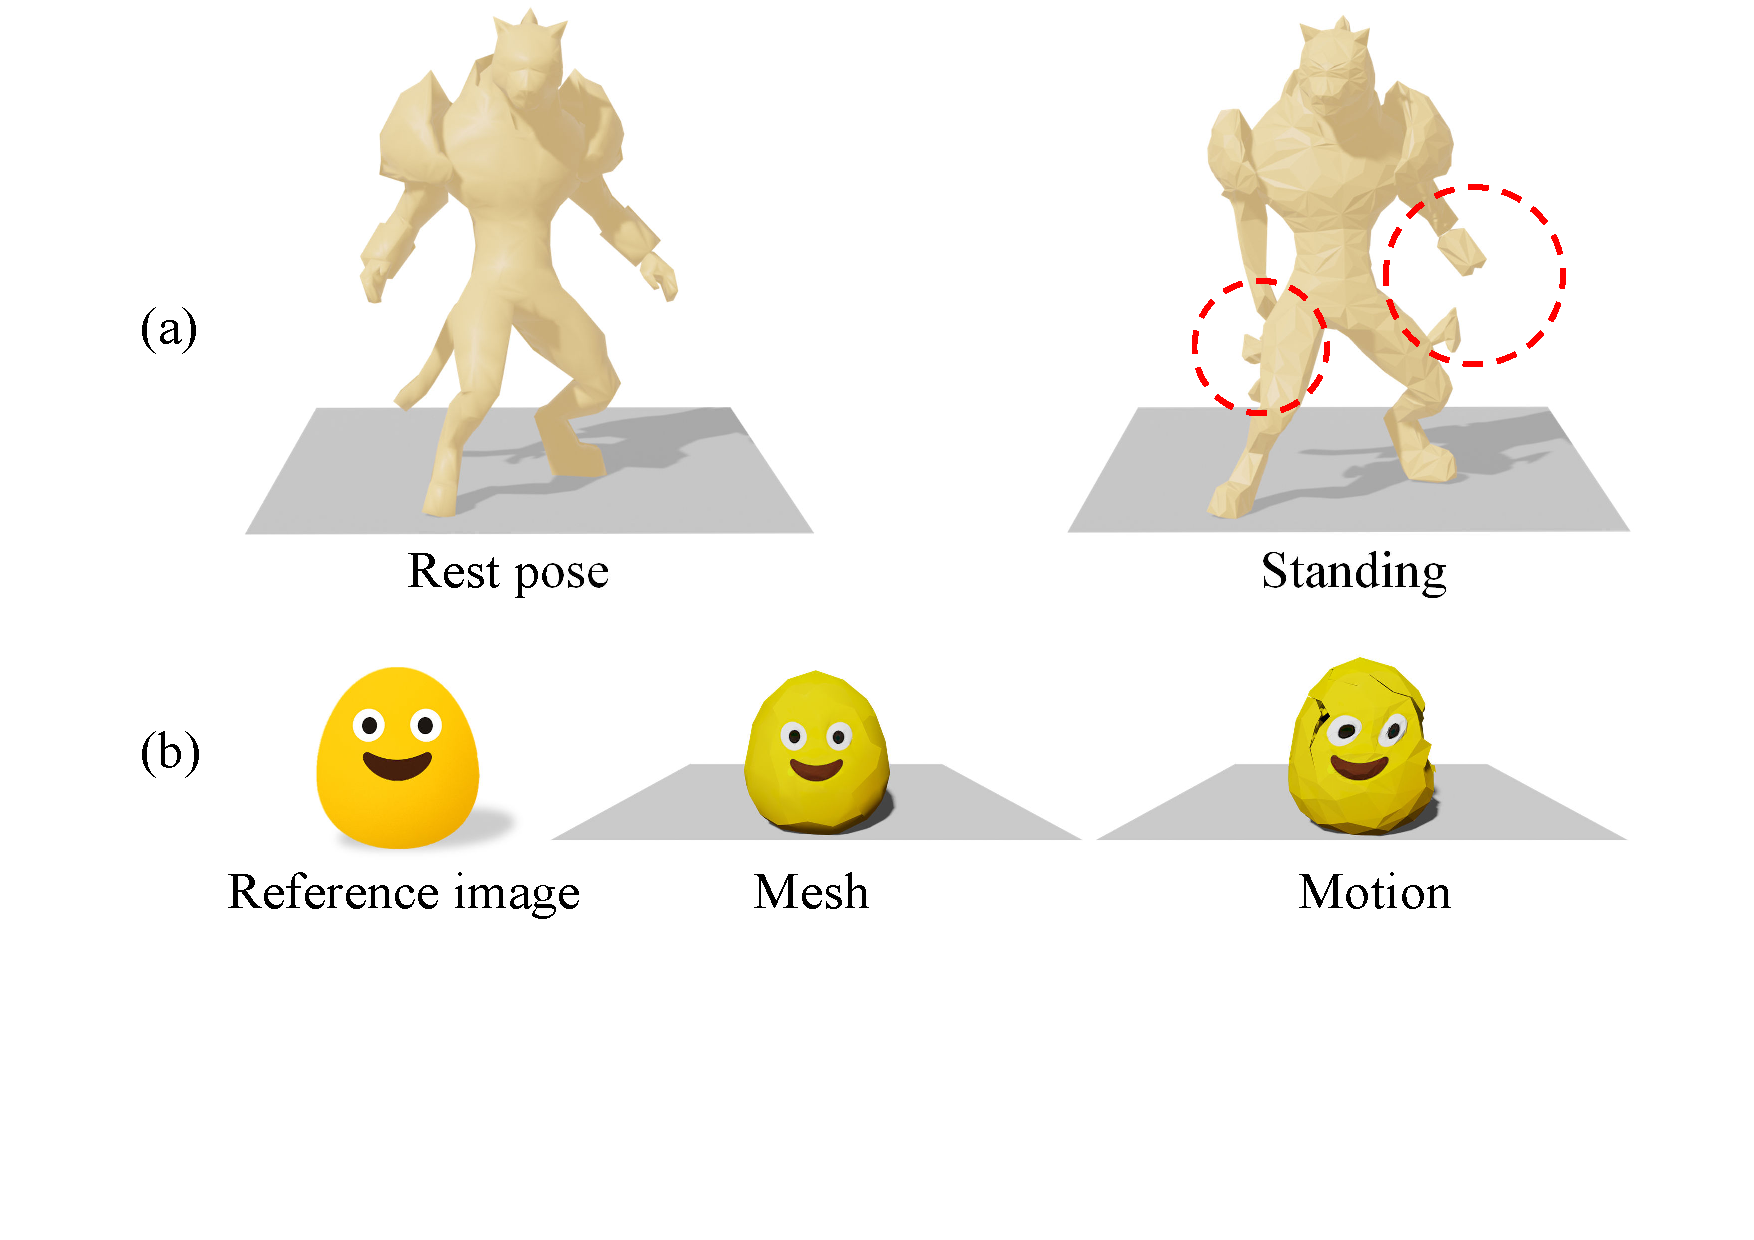
\includegraphics[width=1.0\linewidth]{figure/fig13.pdf}
  \caption{\textbf{A failure case.} For some non-human characters, it is difficult or even impossible to generate a proper rest-pose mesh, and when the rest pose of the character is non-standard, the generated animation exhibits noticeable mesh distortion and breakage.}
  \label{fig:fig13}
  \vspace{-0.7cm}  % Adjust this value to reduce the gap
\end{figure}
Figure \ref{fig:fig13} illustrates a failure case of TapMeMo, where the character animation exhibits noticeable mesh distortion and breakage. For example (a), the issue is caused by the character’s non-standard rest pose, which deviates from the typical T-pose used in our training data. For example (b), due to the limitations of ControlNet, it is unable to generate a rest-pose mesh for some non-human characters without hands or feet, ultimately resulting in severe mesh distortion and breakage in the generated animation. Consequently, TapMeMo faces limitations in generating animations for characters with non-standard rest-poses. It is important to note that this bias related to different rest-poses is not unique to our method, as traditional animation creation also requires consistent rest-poses for target characters. Addressing this bias and finding solutions for character rest-pose variations is an essential area for further research in the field of learning-based animation.

\subsection{Stage Interaction} \label{sec:interaction}
Sec.~\ref{sec:unified} argued that a cascade of a generator and an animator has a vanishing
mixed second derivative between the two stages, and that the coupling terms of
Eq.~\ref{Eq.unified} remove this property. Whether the two stages are in fact inseparable is
an empirical question, and we measure it rather than assert it. Let $Q$ be a quality measure
of the final animation, $A^{\star}$ and $B^{\star}$ our generator and motion model, and
$A_{0}$, $B_{0}$ substitutes drawn from existing systems. We report the interaction term of
the resulting $2\times2$ factorial design,
\begin{equation} \label{Eq.syn}
\Delta_{\text{syn}}=
\big[Q(A^{\star},B^{\star})-Q(A_{0},B^{\star})\big]-
\big[Q(A^{\star},B_{0})-Q(A_{0},B_{0})\big].
\end{equation}
If the two stages were independent contributions, replacing one of them would shift $Q$ by the
same amount regardless of the other, and $\Delta_{\text{syn}}$ would vanish up to noise. A
significant non-zero $\Delta_{\text{syn}}$ therefore measures precisely the quantity that a
cascade cannot produce. We instantiate $A_{0}$ with TRELLIS \cite{xiang2025structured},
TripoSG \cite{li2025triposg} and Hunyuan3D~2.1 \cite{hunyuan3d2025hunyuan3d}, and $B_{0}$ with
UniMate \cite{mou2026unimate}, AnimateAnyMesh \cite{wu2025animateanymesh} and
AnyTop~$+$~LBS \cite{gat2025anytop}. Because QEM decimation and isotropic remeshing are
generic operations that could be applied to any mesh, they enter the design as an explicit
factor: every cell is evaluated both with and without them, and the identical post-processing
is applied to the substitute meshes, so that the effect of the proposed initialisation is
separated from the effect of the subsequent geometry processing. The rest-pose Gaussian
initialisation is likewise contrasted against a standard spherical initialisation with the
remainder of the pipeline unchanged.

% =====================================================================
% c123rev: Table~\ref{table:interaction} now holds measured values
% (experiments_c123/results/factorial2/factorial2.json and results/factorial/).
% TODO(authors): Table~\ref{table:interaction} must be filled with measured
% values. The cells below are placeholders and MUST NOT be reported as results.
% Required runs per cell: {A in [ours, TRELLIS, TripoSG, Hunyuan3D]}
%   x {B in [ours, UniMate, AnimateAnyMesh, AnyTop+LBS]}
%   x {post-processing in [on, off]} x {init in [rest-pose, sphere]}
% Report Self-int. (primary), ARAP Err., Anim. Fail. and CLIP-Sim per cell,
% then Delta_syn of Eq.~\ref{Eq.syn} with a paired bootstrap CI.
% =====================================================================

\begin{revblock}
\textbf{Measured interaction.} Table~\ref{table:interaction} reports two instantiations of the
design with components we could run end to end. Both start from the same off-the-shelf generator,
Hunyuan3D-2mini \cite{zhao2025hunyuan3d}, fed with images from SD1.5 \cite{rombach2022high}, and
compare our animator B$^{\star}$ (Mesh Handle Predictor and Shape-aware Motion Diffusion) with
AnimateAnyMesh \cite{wu2025animateanymesh} as B$_{0}$; the evaluation motions are 4 prompts that
are not used anywhere else. (a) \textit{Coupling term.} On 32 generated characters (16 prompts,
each with and without a T-pose condition, after QEM and remeshing), A$^{\star}$ applies the
animatability prior of Eq.~\ref{Eq.anim} to the generated geometry: 150 Adam steps move the rest
vertices to minimise the frame-averaged squared edge-length change under our field and under
motions sampled from our motion model for 8 other prompts, so that the gradient reaches the
geometry through the deformation operator, with a fidelity and a Laplacian term that limit the
mean vertex displacement to 0.2\% of the body height. As a control for generic geometry
processing, A$_{g}$ applies Taubin smoothing of the same mean displacement. The coupling lowers
the failure rate of our animator from 27\% to 15\% and its self-intersection from $5.1$ to $4.0$
points, and leaves AnimateAnyMesh unchanged or slightly worse; all three interaction terms are
negative with 95\% intervals that exclude zero. Smoothing of the same size leaves the failure
rate of our animator at 27\%, slightly raises its distortion and lowers its self-intersection to
$4.7$ points; its interaction terms on distortion and self-intersection are not distinguishable
from zero, and the one on the failure rate ($-7$ points) comes from AnimateAnyMesh failing more
often after smoothing. The asset is thus improved for the
animator it was coupled to, and only for that one, which is the non-vanishing mixed derivative
of Eq.~\ref{Eq.mixed} that a cascade cannot produce. The result does not rest on measures that
are close to the coupling objective: bending, the change of the dihedral angle at the interior
edges, falls from $5.1^{\circ}$ to $4.2^{\circ}$ for our animator and rises from $3.7^{\circ}$ to
$4.0^{\circ}$ for AnimateAnyMesh ($\Delta_{\text{syn}}=-1.20^{\circ}$, $[-1.57,-0.82]$), against
$-0.31^{\circ}$ ($[-0.73,0.13]$) for smoothing of the same size; the change of the enclosed volume
has the same sign but is not significant; and the mean vertex displacement stays between $0.076$
and $0.078$ for both animators, so the improvement does not come from moving less.
(b) \textit{Rest-pose condition only.}
Without the coupling term, A$^{\star}$ differs from A$_{0}$ only by a ControlNet
\cite{zhang2023adding} conditioned on the canonical T-pose skeleton. On 16 characters, with
post-processing as an additional factor (QEM to 5,000 faces and remeshing to about 2,500
vertices, or QEM to 4,096 vertices only), no interaction term is distinguishable from zero, and
post-processing is the factor that matters for our animator (failure rate from 41\% to 31\% and
from 50\% to 28\%). The inseparability therefore comes from the coupling term, not from the
pose condition. The coupling is applied here as a refinement of extracted meshes rather than
inside the Gaussian generator, and Pose-SDS is not part of this test.
\end{revblock}

\begin{table*}[t]
  \centering
  \color{red}
  \setlength{\abovecaptionskip}{0.5mm}
  \setlength{\tabcolsep}{2.5pt}
  \renewcommand{\arraystretch}{1.2}
  \scriptsize
  \caption{\rev{\textbf{Stage interaction} (Eq.~\ref{Eq.syn}). (a) Coupling term: 32 generated
  characters $\times$ 4 held-out motions; A$^{\star}$ = animatability prior (Eq.~\ref{Eq.anim})
  applied to the generated mesh through our field and motion model, A$_{g}$ = Taubin smoothing of
  the same size, A$_{0}$ = no coupling. (b) Rest-pose condition only: 16 characters $\times$ 4
  motions, A$^{\star}$ = T-pose-conditioned images, with and without post-processing. Dist.:
  length-weighted relative edge change; S-i.: increase of the self-intersecting face fraction over
  the rest mesh (points); Fail.: Dist. $>0.10$. Lower is better; $\Delta_{\text{syn}}<0$ means
  that the change of the generator helps our animator more than B$_{0}$. Brackets: 95\%
  bootstrap intervals over characters.}}
  \label{table:interaction}
  \begin{tabular*}{\textwidth}{@{\extracolsep{\fill}} l c c c c c c}
    \toprule[1.5pt]
    \textbf{(a) Coupling term} & \multicolumn{3}{c}{\textbf{B$^{\star}$ (ours)}} & \multicolumn{3}{c}{\textbf{B$_{0}$ (AnimateAnyMesh)}} \\
    \cmidrule(lr){2-4} \cmidrule(lr){5-7}
    \textbf{Generator} & \textbf{Dist.} & \textbf{S-i.} & \textbf{Fail.} & \textbf{Dist.} & \textbf{S-i.} & \textbf{Fail.} \\
    \midrule[0.5pt]
    A$_{0}$, no coupling          & 0.086 & 5.1 & 27\% & 0.069 & 1.8 & 21\% \\
    A$^{\star}$, coupled          & \textbf{0.063} & \textbf{4.0} & \textbf{15\%} & 0.069 & 2.0 & 26\% \\
    A$_{g}$, generic smoothing    & 0.088 & 4.7 & 27\% & 0.070 & 1.7 & 28\% \\
    \midrule[0.5pt]
    & \multicolumn{2}{c}{$\Delta_{\text{syn}}$ Dist.} & \multicolumn{2}{c}{$\Delta_{\text{syn}}$ S-i.} & \multicolumn{2}{c}{$\Delta_{\text{syn}}$ Fail.} \\
    \cmidrule(lr){2-3} \cmidrule(lr){4-5} \cmidrule(lr){6-7}
    A$^{\star}$ vs.\ A$_{0}$ & \multicolumn{2}{c}{$-0.023$ {[}$-0.034$, $-0.010${]}} & \multicolumn{2}{c}{$-1.4$ {[}$-2.1$, $-0.8${]}} & \multicolumn{2}{c}{$-17$ {[}$-28$, $-8${]}} \\
    A$_{g}$ vs.\ A$_{0}$     & \multicolumn{2}{c}{$+0.000$ {[}$-0.011$, $0.014${]}} & \multicolumn{2}{c}{$-0.4$ {[}$-1.0$, $0.3${]}} & \multicolumn{2}{c}{$-7$ {[}$-14$, $-1${]}} \\
    \bottomrule[1.5pt]
  \end{tabular*}
  \vspace{1mm}

  \begin{tabular*}{\textwidth}{@{\extracolsep{\fill}} l c c c c c c}
    \toprule[1.5pt]
    \textbf{(b) Rest-pose condition} & \multicolumn{3}{c}{\textbf{Post-proc. on}} & \multicolumn{3}{c}{\textbf{Post-proc. off}} \\
    \cmidrule(lr){2-4} \cmidrule(lr){5-7}
    \textbf{Cell} & \textbf{Dist.} & \textbf{S-i.} & \textbf{Fail.} & \textbf{Dist.} & \textbf{S-i.} & \textbf{Fail.} \\
    \midrule[0.5pt]
    A$^{\star}$, B$^{\star}$ & 0.083 & 5.9 & 31\% & 0.098 & 6.1 & 41\% \\
    A$_{0}$, B$^{\star}$     & 0.089 & 4.5 & 28\% & 0.114 & 5.6 & 50\% \\
    A$^{\star}$, B$_{0}$     & 0.051 & 1.4 & 19\% & 0.066 & 2.2 & 33\% \\
    A$_{0}$, B$_{0}$         & 0.086 & 2.1 & 23\% & 0.074 & 2.3 & 22\% \\
    \midrule[0.5pt]
    $\Delta_{\text{syn}}$ & $+0.029$ & $+2.1$ & $+8$ & $-0.007$ & $+0.6$ & $-20$ \\
    95\% interval & {[}$-0.017$, $0.076${]} & {[}$-0.2$, $4.6${]} & {[}$-22$, $42${]} & {[}$-0.049$, $0.034${]} & {[}$-1.6$, $3.1${]} & {[}$-52$, $11${]} \\
    \bottomrule[1.5pt]
  \end{tabular*}
\end{table*}

\begin{revblock}
\textbf{Post-processing as a factor.} Part (b) of Table~\ref{table:interaction} singles out
post-processing as the factor that matters for our animator. Table~\ref{table:postproc} repeats
this test on the meshes that four generators produce from the T-pose-conditioned images of
Table~\ref{table:interaction}, Hunyuan3D-2mini \cite{zhao2025hunyuan3d}, Hunyuan3D~2.1
\cite{hunyuan3d2025hunyuan3d}, TripoSG \cite{li2025triposg} and TRELLIS \cite{xiang2025structured},
and against three substitute animators: AnimateAnyMesh \cite{wu2025animateanymesh} and, since a
generated character carries no artist rig, AnyTop \cite{gat2025anytop} and UniMate
\cite{mou2026unimate} driving a template skeleton through distance-based skinning. With
post-processing on (QEM to 5,000 faces and isotropic remeshing to about 2,500 vertices) instead of
off (QEM to 8,000 faces only), the failure rate of our animator falls on every generator, by 8 to
16 points, whereas none of the substitutes improves consistently: AnyTop fails more often on all
four generators, and AnimateAnyMesh and UniMate change in both directions. The interaction of
Eq.~\ref{Eq.syn} between post-processing and the animator is negative for bending in all 12
generator--animator pairs and for the failure rate in 8 of them, with 95\% intervals that exclude
zero, and none of these interactions is significantly positive. The processing of
Sec.~\ref{3Dmesh} therefore serves the animator it was designed for, as P3 and P4 predict, rather
than improving the meshes in general.
\end{revblock}

\begin{table*}[t]
  \centering
  \color{red}
  \setlength{\abovecaptionskip}{0.5mm}
  \setlength{\tabcolsep}{3pt}
  \renewcommand{\arraystretch}{1.2}
  \scriptsize
  \caption{\rev{\textbf{Post-processing as a factor} on the meshes of four generators (16 characters
  $\times$ 4 held-out motions each). Change of the failure rate, in points, when QEM decimation and
  isotropic remeshing are switched on (QEM to 5,000 faces and remeshing to about 2,500 vertices,
  against QEM to 8,000 faces only), for our animator and for three substitutes (AAM:
  AnimateAnyMesh; AnyTop and UniMate drive a template skeleton through distance-based skinning).
  $\Delta_{\text{syn}}$: interaction of Eq.~\ref{Eq.syn} between post-processing and the animator,
  on the failure rate (points) and on bending (degrees); $\Delta_{\text{syn}}<0$ means that
  post-processing helps our animator more than the substitute. Bold: 95\% bootstrap interval over
  characters excludes zero.}}
  \label{table:postproc}
  \begin{tabular*}{\textwidth}{@{\extracolsep{\fill}} l c c c c c c c c c c}
    \toprule[1.5pt]
    & \multicolumn{4}{c}{\textbf{Change of Fail.} (off $\to$ on)} & \multicolumn{3}{c}{$\Delta_{\text{syn}}$, \textbf{Fail.}} & \multicolumn{3}{c}{$\Delta_{\text{syn}}$, \textbf{Bending}} \\
    \cmidrule(lr){2-5} \cmidrule(lr){6-8} \cmidrule(lr){9-11}
    \textbf{Generator} & \textbf{Ours} & \textbf{AAM} & \textbf{AnyTop} & \textbf{UniMate} & \textbf{AAM} & \textbf{AnyTop} & \textbf{UniMate} & \textbf{AAM} & \textbf{AnyTop} & \textbf{UniMate} \\
    \midrule[0.5pt]
    Hunyuan3D-2mini \cite{zhao2025hunyuan3d} & $-$9.4 & $-$14.1 & $+$4.7 & $-$1.6 & $+$4.7 & \textbf{$-$14.1} & $-$7.8 & \textbf{$-$1.5} & \textbf{$-$2.0} & \textbf{$-$1.2} \\
    Hunyuan3D~2.1 \cite{hunyuan3d2025hunyuan3d} & $-$15.6 & $+$1.6 & $+$6.3 & $+$1.6 & \textbf{$-$17.2} & \textbf{$-$21.9} & \textbf{$-$17.2} & \textbf{$-$2.1} & \textbf{$-$2.1} & \textbf{$-$1.3} \\
    TripoSG \cite{li2025triposg} & $-$10.9 & $-$6.3 & $+$3.1 & $+$3.1 & $-$4.7 & \textbf{$-$14.1} & \textbf{$-$14.1} & \textbf{$-$2.4} & \textbf{$-$2.0} & \textbf{$-$1.0} \\
    TRELLIS \cite{xiang2025structured} & $-$7.8 & $+$6.3 & $+$4.7 & 0.0 & \textbf{$-$14.1} & \textbf{$-$12.5} & $-$7.8 & \textbf{$-$2.5} & \textbf{$-$1.4} & \textbf{$-$0.8} \\
    \bottomrule[1.5pt]
  \end{tabular*}
\end{table*}

\begin{revblock}
\textbf{Our generator in the same design.} The tests above take their meshes from off-the-shelf
generators. To place our own generator in the same design, we implemented the Pose-aware Mesh
Generator of Sec.~\ref{3Dmesh} with the publicly available multi-view prior MVDream
\cite{shi2024mvdream} in place of the camera-adapted SDXL: the Gaussians are initialised on the
canonical T-pose body and optimised by score distillation for 1,200 steps, the animatability prior of
Eq.~\ref{Eq.anim} and pose distillation (Eq.~\ref{Eq.posesds}) act after densification, and the
occupancy passed to Marching Cubes is obtained by visibility carving, a voxel being empty when at
least 8 of 64 rendered views see past it (at the depth where the accumulated opacity of the pixel
reaches 0.15), instead of by thresholding the Gaussian density. The extraction parameters were
chosen by the agreement between mesh and Gaussians alone, and the post-processing is that of
Sec.~\ref{3Dmesh}. Table~\ref{table:gengrid} compares this generator with the four off-the-shelf
generators on the 16 prompts of Table~\ref{table:postproc}, the off-the-shelf generators receiving
the T-pose image of each prompt, under the same post-processing, held-out motions and animators.
Our animator fails on 21.9\% of the clips on our meshes, against 29.7--32.8\% on those
of Hunyuan3D-2mini, Hunyuan3D~2.1 and TripoSG and 18.8\% on those of TRELLIS, and on our meshes
its self-intersection (4.2 points against 5.1--10.3), bending
($4.6^{\circ}$ against $5.1^{\circ}$--$5.8^{\circ}$) and mean squared edge-length change
($0.22$ against $0.31$--$0.40$, $\times10^{-4}$) are the lowest of the five
generators. Replacing TripoSG or TRELLIS by our generator lowers the self-intersection of our
animator more than that of each of the three substitute animators ($\Delta_{\text{syn}}$ from
$-$2.4 to $-$5.2 points, all six 95\% intervals excluding zero), and for the failure rate
the replacement favours our animator in 11 of the 12 generator--substitute pairs, significantly
against AnimateAnyMesh on Hunyuan3D-2mini ($-$15.6 points) and against AnyTop on
TripoSG ($-$23.4 points). Post-processing acts on our meshes as
on the others: it lowers the failure rate of our animator from 32.8\% to 21.9\%, and its
interaction with the animator is negative for bending against all three substitutes
($-1.2^{\circ}$ to $-1.4^{\circ}$) and for the failure rate against AnyTop
($-$20.3 points), all with 95\% intervals that exclude zero. Because the generator and
the extraction differ from those behind Table~\ref{table:readiness}, the two tables are not
comparable. Fig.~\ref{fig:gen_e2e} shows characters of this generator driven end to end and
Fig.~\ref{fig:gen_animators} two of them under four animators.
\end{revblock}

\begin{table*}[t]
  \centering
  \color{red}
  \setlength{\abovecaptionskip}{0.5mm}
  \setlength{\tabcolsep}{3pt}
  \renewcommand{\arraystretch}{1.2}
  \scriptsize
  \caption{\rev{\textbf{Our generator against four off-the-shelf generators} (16 prompts $\times$ 4
  held-out motions, post-processing on). Ours: the implementation of Sec.~\ref{3Dmesh} described in
  the text (MVDream prior, rest-pose initialisation, animatability prior and pose distillation,
  visibility-carved extraction); the off-the-shelf generators receive the SD1.5 T-pose image of the
  same prompt. Left: our animator B$^{\star}$ on the meshes of each generator (Fail.: Dist.\ $>0.10$;
  S-i.: increase of the self-intersecting face fraction over the rest mesh, points; Bend.: change of the
  dihedral angle at interior edges, degrees; ARAP: mean squared edge-length change, $\times10^{-4}$).
  Right: $\Delta_{\text{syn}}$ of Eq.~\ref{Eq.syn} for replacing that generator by ours, against each
  substitute animator (AAM: AnimateAnyMesh; AnyTop and UniMate drive a template skeleton through
  distance-based skinning); $\Delta_{\text{syn}}<0$ means that the replacement helps our animator
  more than the substitute. Bold: 95\% bootstrap interval over characters excludes zero.}}
  \label{table:gengrid}
  \begin{tabular*}{\textwidth}{@{\extracolsep{\fill}} l c c c c c c c c c c c}
    \toprule[1.5pt]
    & \multicolumn{5}{c}{\textbf{B$^{\star}$ on the meshes of the generator}} & \multicolumn{3}{c}{$\Delta_{\text{syn}}$, \textbf{Fail.} (points)} & \multicolumn{3}{c}{$\Delta_{\text{syn}}$, \textbf{S-i.} (points)} \\
    \cmidrule(lr){2-6} \cmidrule(lr){7-9} \cmidrule(lr){10-12}
    \textbf{Generator} & \textbf{Fail.} & \textbf{S-i.} & \textbf{Dist.} & \textbf{Bend.} & \textbf{ARAP} & \textbf{AAM} & \textbf{AnyTop} & \textbf{UniMate} & \textbf{AAM} & \textbf{AnyTop} & \textbf{UniMate} \\
    \midrule[0.5pt]
    Hunyuan3D-2mini \cite{zhao2025hunyuan3d} & 31.3\% & 5.9 & 0.083 & 5.1 & 0.31 & \textbf{$-$15.6} & $-$12.5 & $-$12.5 & $-$1.4 & \textbf{$-$3.3} & $-$0.2 \\
    Hunyuan3D~2.1 \cite{hunyuan3d2025hunyuan3d} & 32.8\% & 5.1 & 0.089 & 5.2 & 0.40 & $-$14.1 & $-$12.5 & $-$12.5 & $-$0.7 & $-$0.3 & $+$1.1 \\
    TripoSG \cite{li2025triposg} & 29.7\% & 8.7 & 0.091 & 5.8 & 0.34 & $-$15.6 & \textbf{$-$23.4} & $-$12.5 & \textbf{$-$3.8} & \textbf{$-$5.2} & \textbf{$-$2.8} \\
    TRELLIS \cite{xiang2025structured} & 18.8\% & 10.3 & 0.080 & 5.3 & 0.33 & $+$7.8 & $-$14.1 & $-$4.7 & \textbf{$-$2.7} & \textbf{$-$2.4} & \textbf{$-$4.4} \\
    \midrule[0.5pt]
    Ours (implementation of Sec.~\ref{3Dmesh}) & 21.9\% & 4.2 & 0.084 & 4.6 & 0.22 & -- & -- & -- & -- & -- & -- \\
    \bottomrule[1.5pt]
  \end{tabular*}
\end{table*}

\begin{figure*}[t]
\centering
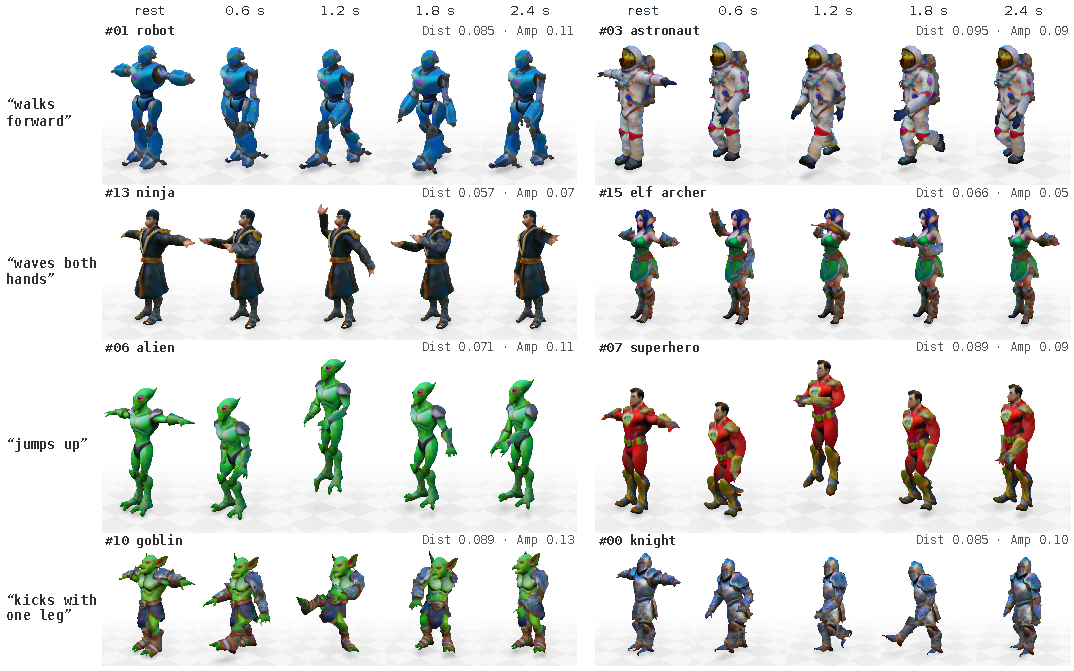
\includegraphics[width=\textwidth]{figure/gen_e2e.pdf}
\caption{\rev{\textbf{Characters of our generator animated end to end.} Each row is one of the four
held-out prompts and shows two of the 16 characters of Table~\ref{table:gengrid} (implementation of
Sec.~\ref{3Dmesh} with the MVDream prior, rest-pose initialisation, both coupling terms,
visibility-carved extraction and post-processing), driven by the Mesh Handle Predictor and the
Shape-aware Motion Diffusion with the root trajectory of the motion model; the camera follows the
root and the floor shows the distance covered. The surface colour is the multi-view rendering of the
Gaussians projected onto the mesh. Dist.: length-weighted relative edge change; Amp.: mean vertex
displacement from the rest pose without the root trajectory; both over the scored frames.}}
\label{fig:gen_e2e}
\end{figure*}

\begin{figure*}[t]
\centering
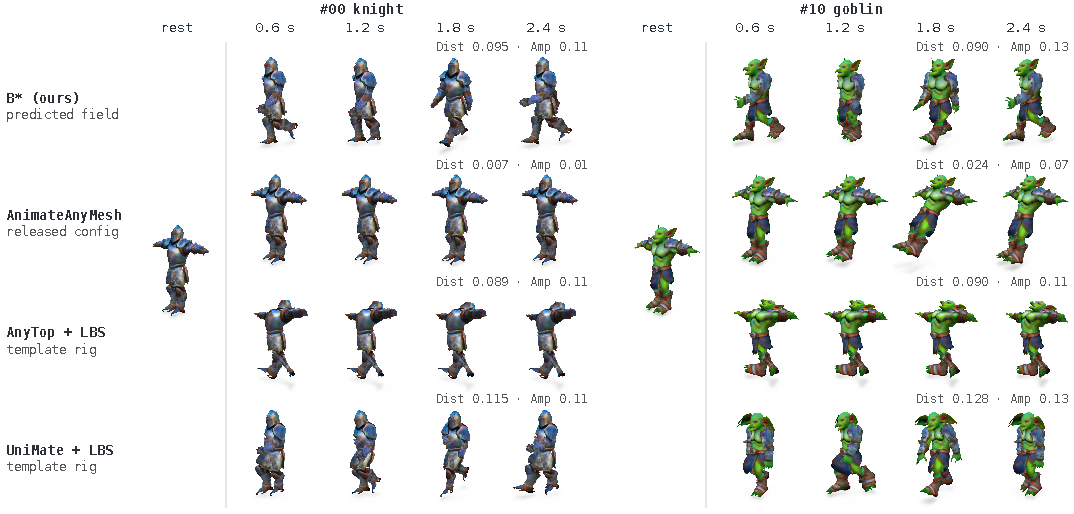
\includegraphics[width=\textwidth]{figure/gen_animators.pdf}
\caption{\rev{\textbf{One mesh, four animators} (``walks forward''). Two characters of our generator
(as in Table~\ref{table:gengrid}) driven by our animator, by AnimateAnyMesh with its released
configuration, and by AnyTop and UniMate on a template skeleton with distance-based skinning, since a
generated character carries no artist rig. Frames at 0.6, 1.2, 1.8 and 2.4\,s of the 15 scored frames;
our animator, AnyTop and UniMate are shown without root translation, AnimateAnyMesh with its own global
motion. Dist.\ and Amp.\ as in Fig.~\ref{fig:gen_e2e}; a result that barely moves also has a small
Dist.}}
\label{fig:gen_animators}
\end{figure*}

\textbf{Verifying the conditions of the drivable manifold}. The four claims of
Sec.~\ref{sec:drivable} are falsifiable individually, and we test them separately rather than
inferring them from end-to-end animation quality.
P1 predicts that driving error grows with the deviation of the input pose from the canonical
one: we take artist-rigged characters, pose them away from the rest pose by a controlled
amount, and measure the composition residual of Eq.~\ref{Eq.resid} against that amount, which
should pass through the origin.
P2 predicts that a spherical initialization leaves the handle channels permuted arbitrarily
per character: we measure channel consistency as the fraction of characters in which channel
$k$ lands on the same semantic part, under rest-pose and spherical initialization, and expect
transfer to collapse in the latter case even when geometric fidelity is unchanged.
P3 predicts a bias in the handle position that grows with the dispersion of the vertex areas:
we compare the plain vertex average of Eq.~\ref{Eq.moment} against the area-weighted estimator
of Eq.~\ref{Eq.quad} as a function of $\mathrm{std}(A_{i})/\bar{A}$, before and after isotropic
remeshing, and additionally report the resulting skinning error.
P4 predicts that channel comparability degrades when $|V|$ is not normalised: we sweep the
decimation budget $V^{\star}$ and report channel consistency and animation failure rate.
Reporting these four together is what separates the proposed conditions from generic geometry
processing, since a generic clean-up step would improve visual quality without producing the
specific dependencies above.

% =====================================================================
% TODO(authors): four plots / one table for P1-P4 as described above.
% P1: composition residual vs. input-pose deviation (should vanish at 0).
% P2: channel consistency, rest-pose init vs. spherical init.
% P3: handle bias and skinning error vs. std(A_i)/mean(A_i), pre/post remeshing.
% P4: channel consistency and Anim. Fail. vs. decimation budget V*.
% =====================================================================

\begin{revblock}
Table~\ref{table:drivable} reports the four tests on the 30 Mixamo test characters with the
pretrained Mesh Handle Predictor and motions sampled from the Shape-aware Motion Diffusion; all
lengths are in units of body height. \textbf{P1.} We pose each character by a generated motion
$\bm{a}$ scaled by $\alpha$, re-run the predictor on the posed mesh as if the asset had been
generated in that pose, and apply a second generated motion $\bm{b}$. The residual of
Eq.~\ref{Eq.resid} is below $10^{-4}$ at $\alpha=0$ and grows faster than the pose deviation,
reaching $0.061$ at a mean vertex displacement of $0.13$. Without re-estimation it stays at
$0.002$, so almost all of it comes from the field estimated on a non-canonical pose, whose
assignment differs from the rest-pose one by a total variation of $0.26$. \textbf{P2.} We emulate
the two initialisations at the level of the field: the canonical gauge is the predictor's
output on the T-pose mesh, and a gauge-free initialisation is the same field with its channels
permuted per character, which no rest-pose objective can distinguish. The geometry and the
rest-pose prior loss are identical, while channel consistency drops from $0.81$ to $0.09$ and the
failure rate under the same channel-indexed motions rises from 19\% to 81\%. This collapse is
expected by construction once the gauge is lost, and it only illustrates the cost of P2. The
informative measurement is the next one: the articulation prior of Sec.~\ref{sec:sensor},
evaluated on the driven characters, prefers the canonical gauge for 93\% of the characters and
picks it out of ten candidates for 87\% (chance 10\%), so the gauge is invisible at rest but
observable under motion. \textbf{P3.} With the artist weights as
the assignment, the bias of the plain vertex average grows with the dispersion of the vertex
areas, from $0.008$ on the original meshes to $0.018$ after three local refinements, whereas the
area-weighted estimator stays at $0.001$ on all triangulations except the decimated one ($0.006$),
whose large triangles make the lumped quadrature inexact. The raw Marching-Cubes surface is
nearly uniform ($\mathrm{CV}=0.38$); QEM decimation makes it non-uniform ($0.94$) and multiplies
the bias by eight, and isotropic remeshing reduces it again by a factor of two. The resulting
driving error follows the same ordering. \textbf{P4.} Below the resolution at which the predictor was trained
(about 2,500 vertices) the failure rate is flat (15--19\%); above it, it rises to 28\%, 43\% and
65\% at 5k, 10k and 20k vertices, while cross-character channel consistency decreases
monotonically from $0.81$ to $0.76$ over the same range. A fixed vertex budget at the training
resolution is therefore a condition for the field, not only for rendering cost.
\end{revblock}

\begin{table*}[t]
  \centering
  \color{red}
  \setlength{\abovecaptionskip}{0.5mm}
  \setlength{\tabcolsep}{3pt}
  \renewcommand{\arraystretch}{1.2}
  \scriptsize
  \caption{\rev{\textbf{The conditions of the drivable manifold} (30 Mixamo test characters, pretrained
  Mesh Handle Predictor, generated motions; lengths in body heights). (a) P1: composition residual
  of Eq.~\ref{Eq.resid} with and without re-estimating the field on the posed mesh, against the
  amplitude $\alpha$ of the first motion. (b) P2: canonical gauge versus the same field with
  channels permuted per character. (c) P3: bias of the plain (Eq.~\ref{Eq.moment}) and
  area-weighted (Eq.~\ref{Eq.quad}) handle estimators and the resulting driving error, per
  triangulation. (d) P4: vertex budget; ``native'' is the training resolution. Fail.: share of
  motions whose length-weighted relative edge change exceeds 0.10.}}
  \label{table:drivable}
  \begin{tabular*}{\textwidth}{@{\extracolsep{\fill}} l c c c c c c c}
    \toprule[1.5pt]
    \textbf{(a) P1}, motion amplitude $\alpha$ & 0 & 0.1 & 0.25 & 0.5 & 0.75 & 1.0 & 1.5 \\
    \midrule[0.5pt]
    Pose deviation $\lVert\bm{p}_{a}-\bm{p}\rVert$ & 0 & 0.013 & 0.033 & 0.066 & 0.100 & 0.133 & 0.198 \\
    Residual, field re-estimated on the posed mesh & $<10^{-4}$ & 0.002 & 0.005 & 0.013 & 0.029 & 0.061 & 0.103 \\
    Residual, field kept (blend skinning only) & $<10^{-4}$ & $<10^{-3}$ & $<10^{-3}$ & 0.001 & 0.002 & 0.002 & 0.003 \\
    Change of the re-estimated field (TV) & $<10^{-3}$ & 0.018 & 0.043 & 0.093 & 0.162 & 0.262 & 0.403 \\
    \bottomrule[1.5pt]
  \end{tabular*}
  \vspace{1mm}

  \begin{tabular*}{\textwidth}{@{\extracolsep{\fill}} l c c c c c c}
    \toprule[1.5pt]
    \textbf{(b) P2}, field gauge & \textbf{Consistency} & \textbf{Rest-pose prior loss} & \textbf{Distortion} & \textbf{Fail.} &
    \textbf{Sensing loss} & \textbf{Gauge recovered} \\
    \midrule[0.5pt]
    Canonical (T-pose initialisation) & \textbf{0.81} & $2.1\times10^{-4}$ & \textbf{0.074} & \textbf{19\%} & \textbf{0.033} & -- \\
    Permuted (no gauge)               & 0.09 & $2.1\times10^{-4}$ & 0.240 & 81\% & 0.069 & 87\% of characters (chance 10\%) \\
    \bottomrule[1.5pt]
  \end{tabular*}
  \vspace{1mm}

  \begin{tabular*}{\textwidth}{@{\extracolsep{\fill}} l c c c c c c c c}
    \toprule[1.5pt]
    \textbf{(c) P3}, triangulation & Orig. & Ref.\,$\times1$ & Ref.\,$\times2$ & Ref.\,$\times3$ & Raw MC & MC$+$QEM &
    MC$+$QEM$+$rem. & Orig.$+$rem. \\
    \midrule[0.5pt]
    $\mathrm{std}(A_{i})/\bar{A}$         & 0.66 & 0.88 & 1.52 & 2.90 & 0.38 & 0.94 & 0.49 & 0.36 \\
    Handle bias, plain average           & 0.0079 & 0.0105 & 0.0143 & 0.0175 & 0.0023 & 0.0181 & 0.0080 & 0.0046 \\
    Handle bias, area-weighted           & 0.0010 & 0.0010 & 0.0009 & 0.0009 & 0.0004 & 0.0056 & 0.0009 & 0.0005 \\
    Driving error, plain average         & 0.0046 & 0.0059 & 0.0082 & 0.0098 & 0.0009 & 0.0038 & 0.0026 & 0.0022 \\
    Driving error, area-weighted         & 0.0009 & 0.0007 & 0.0008 & 0.0006 & 0.0002 & 0.0006 & 0.0003 & 0.0004 \\
    \bottomrule[1.5pt]
  \end{tabular*}
  \vspace{1mm}

  \begin{tabular*}{\textwidth}{@{\extracolsep{\fill}} l c c c c c c c}
    \toprule[1.5pt]
    \textbf{(d) P4}, vertex budget (mean $|V|$) & 1.3k & 1.8k & native 2.5k & 3.0k & 5.4k & 10.3k & 20.1k \\
    \midrule[0.5pt]
    Cross-character channel consistency & 0.79 & 0.78 & \textbf{0.81} & 0.79 & 0.79 & 0.77 & 0.76 \\
    Same-character consistency with native & 0.94 & 0.95 & 1 & 0.95 & 0.92 & 0.91 & 0.90 \\
    Distortion                           & 0.068 & 0.071 & 0.075 & 0.078 & 0.092 & 0.119 & 0.166 \\
    Fail.                                & 15\% & 17\% & 18\% & 19\% & 28\% & 43\% & 65\% \\
    \bottomrule[1.5pt]
  \end{tabular*}
\end{table*}

\subsection{Quantitative Results}
\begin{table*}[t]
  \centering
  \setlength{\abovecaptionskip}{0.5mm}
  \setlength{\belowcaptionskip}{0mm}
  \scriptsize
  \caption{\textbf{Comparison of text-based motion generation on the HumanML3D dataset.}
  \blu{The upper block uses the standard T2M feature space with} ``Real'' \blu{as the
  reference, where prior-work values are taken from their original papers and our starred
  row is our motion mapped onto the SMPL skeleton; the lower block uses our handle-based
  space, where ``Real}\dag{}'' is the real distribution that is extracted from our motion
  representation by the retrained feature extractor. ``TapMeMo (MDM)'' is
  \blu{an} implementation that employs the same diffusion structure as MDM.
  \blu{Values are comparable only within a block. \textbf{Bold} and
  \underline{underline} mark the best and second best in each block, reference rows
  excluded; ``--'' denotes a metric not reported in the original paper.}}
  \label{table:1}
  \begin{tabular*}{\textwidth}{@{\extracolsep{\fill}} l c c c c c c}
    \toprule[1.5pt]
    \textbf{Method} & \textbf{R-Prec. (Top-1)}$_{\uparrow}$ & \textbf{R-Prec. (Top-3)}$_{\uparrow}$ & \textbf{FID}$_{\downarrow}$ & Multimodal Dist$_{\downarrow}$ & Diversity$_{\rightarrow}$ & Multimodality$_{\uparrow}$ \\
    \midrule[0.5pt]
    \multicolumn{7}{l}{\blu{\textit{Standard T2M feature space (reference: Real)}}} \\
    Real & 0.511$^{\pm.003}$ & 0.797$^{\pm.002}$ & 0.002$^{\pm.000}$ & 2.974$^{\pm.008}$ & 9.503$^{\pm.065}$ & \blu{--} \\
    T2G  & 0.165$^{\pm.001}$ & 0.345$^{\pm.002}$ & 7.664$^{\pm.030}$ & 6.030$^{\pm.018}$ & 6.409$^{\pm.071}$ & \blu{--} \\
    Hier & 0.301$^{\pm.002}$ & 0.552$^{\pm.004}$ & 6.532$^{\pm.024}$ & 5.012$^{\pm.018}$ & 8.332$^{\pm.042}$ & \blu{--} \\
    TEMOS & 0.424$^{\pm.002}$ & 0.722$^{\pm.002}$ & 3.734$^{\pm.028}$ & 3.703$^{\pm.008}$ & 8.973$^{\pm.071}$ & 0.368$^{\pm.018}$ \\
    T2M  & 0.457$^{\pm.002}$ & 0.740$^{\pm.003}$ & 1.067$^{\pm.002}$ & 3.340$^{\pm.008}$ & 9.188$^{\pm.002}$ & 2.090$^{\pm.083}$ \\
    MotionDiffuse & 0.491$^{\pm.001}$ & 0.782$^{\pm.001}$ & 0.630$^{\pm.001}$ & 3.113$^{\pm.001}$ & 9.410$^{\pm.049}$ & 1.553$^{\pm.083}$ \\
    MDM  & 0.320$^{\pm.002}$ & 0.611$^{\pm.007}$ & 0.544$^{\pm.044}$ & 5.566$^{\pm.027}$ & \textbf{9.559$^{\pm.086}$} & \textbf{2.799$^{\pm.072}$} \\
    ReMoDiffuse & 0.510$^{\pm.005}$ & 0.795$^{\pm.004}$ & \blu{0.103$^{\pm.004}$} & \blu{2.974$^{\pm.016}$} & 9.018$^{\pm.075}$ & 1.795$^{\pm.043}$ \\
    \blu{MoMask} & \blu{\underline{0.521}$^{\pm.002}$} & \blu{\underline{0.807}$^{\pm.002}$} & \blu{\underline{0.045}$^{\pm.002}$} & \blu{\underline{2.958}$^{\pm.008}$} & \blu{--} & \blu{1.241$^{\pm.040}$} \\
    \blu{MoGenTS} & \blu{\textbf{0.529$^{\pm.003}$}} & \blu{\textbf{0.812$^{\pm.002}$}} & \blu{\textbf{0.033$^{\pm.001}$}} & \blu{\textbf{2.867$^{\pm.006}$}} & \blu{\underline{9.570}$^{\pm.077}$} & \blu{--} \\
    \blu{\textbf{TapMeMo (Ours)}$^{\ast}$} & \blu{0.503$^{\pm.004}$} & \blu{0.789$^{\pm.002}$} & \blu{0.414$^{\pm.037}$} & \blu{5.180$^{\pm.045}$} & \blu{9.210$^{\pm.068}$} & \blu{\underline{2.320}$^{\pm.032}$} \\
    \midrule[0.5pt]
    \multicolumn{7}{l}{\blu{\textit{Handle-based representation, retrained extractor (reference: Real\dag{})}}} \\
    Real\dag & 0.559$^{\pm.007}$ & 0.828$^{\pm.005}$ & 0.002$^{\pm.001}$ & 4.371$^{\pm.035}$ & 17.176$^{\pm.178}$ & \blu{--} \\
    TapMeMo (MDM) & 0.498$^{\pm.006}$ & \blu{\underline{0.801}}$^{\pm.003}$ & 1.058$^{\pm.056}$ & 5.126$^{\pm.069}$ & 16.553$^{\pm.315}$ & \blu{\textbf{2.744$^{\pm.156}$}} \\
    \blu{\textbf{TapMeMo (Ours)}} & \textbf{0.542$^{\pm.008}$} & \textbf{0.805$^{\pm.002}$} & \blu{\textbf{0.515$^{\pm.088}$}} & \blu{\textbf{5.058$^{\pm.063}$}} & \blu{\textbf{16.724$^{\pm.380}$}} & \blu{\underline{2.559}}$^{\pm.230}$ \\
    \bottomrule[1.5pt]
  \end{tabular*}
\end{table*}

\begin{table}[t]
  \centering
  \setlength{\abovecaptionskip}{0.5mm}
  \setlength{\belowcaptionskip}{0mm}
  \renewcommand{\arraystretch}{1.3}
  \scriptsize
  \setlength{\tabcolsep}{0pt}
  \caption{\textbf{Comparison of mesh distortion.} ``Self-int.'' \blu{denotes the
  self-intersection rate, which we use as the primary geometry metric, and ``ARAP Err.'' is
  reported only as a secondary reference.} ``w/ \blu{$\mathcal{L}_h$'' and ``w/ $\mathcal{L}_a$''
  add the Spring Loss and the Adversarial Loss, respectively, on top of the} ``w/o $\delta$\blu{''
  variant. ``w/o $\delta$} ft'' means results without adaptation fine-tuning. ``S'' and
  ``U'' represent seen and unseen characters.}
  \label{table:2}
  \begin{tabular*}{\linewidth}{@{\extracolsep{\fill}} l ccccc @{}}
    \toprule[1.5pt]
    \textbf{Methods} & \multicolumn{2}{c}{\blu{\textbf{Self-int.} (\%)$_{\downarrow}$}}
                     & \multicolumn{2}{c}{\blu{\textbf{ARAP Err.}$_{\downarrow}$}}
                     & \textbf{\blu{Handle-}} \\
    \cmidrule(lr){2-3} \cmidrule(lr){4-5}
                     & \blu{S} & \blu{U} & \blu{S} & \blu{U} & \blu{\textbf{FID}}$_{\downarrow}$ \\
    \midrule[0.5pt]
    MDM-SR  & \blu{3.85} & \blu{4.32} & 0.897 & 0.787 & \textbf{0.012} \\
    MDM-SFR & \blu{5.12} & \blu{5.86} & 1.006 & 0.910 & 0.163 \\
    \midrule[0.5pt]
    TapMeMo (w/o $\delta$)         & \blu{2.15} & \blu{2.68} & 0.310 & 0.356 & 0.055 \\
    TapMeMo (w/ $\mathcal{L}_{h}$) & \blu{1.62} & \blu{2.08} & 0.303 & 0.347 & 0.048 \\
    TapMeMo (w/ $\mathcal{L}_{a}$) & \blu{1.70} & \blu{2.15} & 0.307 & 0.342 & 0.056 \\
    TapMeMo (w/o $\delta$ ft)      & \blu{1.48} & \blu{1.88} & 0.301 & 0.335 & 0.048 \\
    TapMeMo (Ours)                 & \blu{\textbf{1.12}} & \blu{\textbf{1.45}} & \textbf{0.271}
                                   & \textbf{0.329} & \underline{0.046} \\
    \bottomrule[1.5pt]
  \end{tabular*}
\end{table}

Table \ref{table:1} provides a quantitative comparison between our TapMeMo and the previous
motion generation models, including T2G \cite{bhattacharya2021text2gestures}, Hier
\cite{ghosh2021synthesis}, TEMOS \cite{petrovich2022temos}, T2M \cite{guo2022generating},
MDM \cite{tevet2022human}, \blu{ReMoDiffuse \cite{zhang2023remodiffuse}, MoMask
\cite{guo2024momask} and MoGenTS \cite{yuan2024mogents}. The table is organised into two blocks that must
be read separately. The upper block reports the standard T2M feature space, in which our
generated handle motion is first mapped onto the SMPL skeleton so that the pre-trained
extractor of \cite{guo2022generating} applies; the lower block reports our handle-based
space with the retrained extractor. In the upper block, the recent masked-token methods
MoMask and MoGenTS achieve the strongest scores, which is expected since they are designed
and trained directly on the SMPL skeleton that this feature space assumes. Our starred row
reaches an FID of 0.414 and a Top-3 of 0.789, remaining competitive with the diffusion-based
methods (0.630 for MotionDiffuse and 0.544 for MDM) even though our motion is not generated
on a fixed skeleton and must be converted before evaluation; this conversion is also the
main source of our higher Multimodal Dist. In the lower block, where every entry shares our
representation, our} TapMeMo outperforms the previous models significantly in terms of both
R-Precision and FID metrics. Besides, the introduced multi-token and Transformer Decoder
strategies that to the Shape-aware Motion Diffusion, showed a stable improvement in all
metrics. Notably, TapMeMo (Ours) achieved a remarkable improvement of over 50\% in the FID
metric compared to the TapMeMo (MDM) implementation, with a score of 0.515 vs 1.058. These
findings demonstrate the superior performance of our TapMeMo and the effectiveness of the
adaptations we made to the Diffusion Model structure, which allowed for more accurate and
higher-quality motion generation.

Table \ref{table:2} provides a comprehensive comparison between TapMeMo and the baseline methods, focusing on the geometry quality of the generated animations. TapMeMo demonstrates remarkable improvements, achieving a significant reduction in ARAP-Loss both on seen and unseen characters. Specifically, TapMeMo achieves 69.8\% (0.271 vs. 0.897) lower scores compared to MDM-SR and 73.1\% (0.271 vs. 1.006) lower scores compared to MDM-SFR on seen characters. For unseen characters, TapMeMo achieves 58.2\% (0.329 vs. 0.787) lower scores compared to MDM-SR and 63.8\% (0.329 vs. 0.910) lower scores compared to MDM-SFR. These results indicate that TapMeMo excels in generating animations with superior geometry details and smoother mesh surfaces compared to the baseline methods. Moreover, TapMeMo exhibits a superior global geometry preservation performance, with Handle-FID scores 71.7\% (0.046 vs 0.163) lower than MDM-SFR. Notably, MDM-SR achieves the best Handle-FID (0.012) due to its utilization of a standard SMPL skeleton structure, resulting in minimal global distortion when driving the SMPL model. Additionally, the ablative study underscores the effectiveness of the special designs employed in our TapMeMo pipeline.


\blu{Table~\ref{table:rigfree} compares TapMeMo with two recent rig-free animation methods:
AnyTop~\cite{gat2025anytop}, whose skeletal motion we bind to the mesh with LBS, and
AnimateAnyMesh~\cite{wu2025animateanymesh}, which deforms a given mesh from text. As they assume
different mesh resolutions and sequence lengths, all methods are evaluated on meshes
decimated to 4,096 vertices and on 16-frame clips; the absolute values are thus not
comparable with Table~\ref{table:2}. Against the stronger baseline, TapMeMo lowers the
self-intersection rate by 66.3\% (0.95 vs.\ 2.82) on seen and 64.0\% (1.28 vs.\ 3.56) on
unseen characters, with 43.7\% and 41.8\% lower ARAP Error. Both baselines require an
external input---a predefined skeleton that cannot cover arbitrary topologies, or per-vertex
displacements without a control structure---whereas our handles are predicted from the mesh
itself and shared across frames, which keeps the deformation consistent on unseen topologies.}

\begin{revblock}
\textbf{Re-measurement under one protocol.} AnimateAnyMesh must be sampled with the latent
normalisation of its released configuration; without it the decoded vertex trajectories are
torn apart (median relative edge change above 100\% on its own example). We therefore re-ran
both systems with the released configuration on the same meshes, 15 seen (Mixamo training) and
15 unseen (Mixamo test) characters with 4 motion prompts each, and report the result in
Table~\ref{table:rigfree2}. Our animator keeps its advantage on seen characters (self-intersection
increase $2.6$ against $4.3$ points, failure rate 17\% against 37\%), where AnimateAnyMesh also
moves twice as much. On unseen characters the ordering reverses: AnimateAnyMesh distorts less
($0.061$ against $0.082$) and fails less often (18\% against 32\%) with smaller motions. The
values of Table~\ref{table:rigfree} for AnimateAnyMesh are not reproduced by this protocol.
\end{revblock}

\begin{table}[t]
  \centering
  \color{red}
  \setlength{\abovecaptionskip}{0.5mm}
  \setlength{\tabcolsep}{2.5pt}
  \renewcommand{\arraystretch}{1.2}
  \scriptsize
  \caption{\rev{\textbf{Rig-free baseline re-measured} with the released configuration of
  AnimateAnyMesh, on the same meshes (15 seen and 15 unseen Mixamo characters $\times$ 4 motions).
  S-i.: increase of the self-intersecting face fraction over the rest mesh (points); ARAP: mean
  squared edge-length change ($\times10^{4}$, body height $=1$); Dist.: length-weighted relative
  edge change; Fail.: Dist. $>0.10$; Disp.: mean vertex displacement (AnimateAnyMesh includes the
  global trajectory, ours does not).}}
  \label{table:rigfree2}
  \begin{tabular*}{\linewidth}{@{\extracolsep{\fill}} l l c c c c c}
    \toprule[1.5pt]
    & \textbf{Method} & \textbf{S-i.}$_{\downarrow}$ & \textbf{ARAP}$_{\downarrow}$ & \textbf{Dist.}$_{\downarrow}$ & \textbf{Fail.}$_{\downarrow}$ & \textbf{Disp.} \\
    \midrule[0.5pt]
    Seen   & AnimateAnyMesh & 4.3 & 1.91 & 0.099 & 37\% & 0.285 \\
           & Ours           & \textbf{2.6} & \textbf{0.77} & \textbf{0.068} & \textbf{17\%} & 0.134 \\
    \midrule[0.5pt]
    Unseen & AnimateAnyMesh & \textbf{2.2} & \textbf{0.14} & \textbf{0.061} & \textbf{18\%} & 0.090 \\
           & Ours           & 2.7 & 0.17 & 0.082 & 32\% & 0.115 \\
    \bottomrule[1.5pt]
  \end{tabular*}
\end{table}

\begin{table}[t]
  \centering
  \setlength{\abovecaptionskip}{0.5mm}
  \renewcommand{\arraystretch}{1.3}
  \scriptsize
  \caption{\blu{\textbf{Comparison with rig-free animation baselines}, under aligned
  geometry (4,096 vertices) and length (16 frames); values are therefore not directly
  comparable with Table~\ref{table:2}. ``S''/``U'' denote seen and unseen characters.}}
  \label{table:rigfree}
  \begin{tabularx}{\linewidth}{lXcccc}
    \toprule[1.5pt]
    \blu{\textbf{Method}} & \blu{\textbf{Input}} & \blu{\textbf{S-i.}} & \blu{\textbf{S-i.}} & \blu{\textbf{A-E}} & \blu{\textbf{A-E}} \\
                    &                & \blu{\textbf{(S)}$_{\downarrow}$} & \blu{\textbf{(U)}$_{\downarrow}$}
                    & \blu{\textbf{(S)}$_{\downarrow}$} & \blu{\textbf{(U)}$_{\downarrow}$} \\
    \midrule[0.5pt]
    \blu{AnyTop $+$ LBS}  & \blu{skeleton}     & \blu{3.45} & \blu{4.12} & \blu{0.582} & \blu{0.695} \\
    \blu{AnimateAnyMesh}  & \blu{mesh $+$ text} & \blu{2.82} & \blu{3.56} & \blu{0.435} & \blu{0.512} \\
    \midrule[0.5pt]
    \blu{\textbf{Ours}}   & \blu{text / image} & \blu{\textbf{0.95}} & \blu{\textbf{1.28}} & \blu{\textbf{0.245}} & \blu{\textbf{0.298}} \\
    \bottomrule[1.5pt]
  \end{tabularx}
\end{table}

Table \ref{table:mesh} presents a quantitative comparison of different methods in terms of semantic consistency and generation efficiency, measured by CLIP-Similarity and Generation Time. 
TapMeMo achieves a CLIP-Similarity of 0.742, showing a clear improvement over DreamGaussian (0.738) and Zero-1-to-3 (0.647). 
Compared to inference-only approaches such as One-2-3-45 (0.594), Point-E (0.587), and Shap-E (0.591), TapMeMo demonstrates significantly better semantic alignment with the input text. 
Although Zero-1-to-3$^*$ achieves a higher CLIP-Similarity (0.778), it relies on a costly optimization-based process requiring 30 minutes, whereas TapMeMo delivers comparable quality in just 97 seconds—an efficiency improvement of over 18$\times$. 
This indicates that TapMeMo strikes a favorable balance between generation quality and speed, achieving high semantic alignment while remaining practical for real-world applications.
\begin{table}[t]
  \centering
  \setlength{\abovecaptionskip}{0.5mm}
  \setlength{\belowcaptionskip}{0mm}
  \renewcommand{\arraystretch}{1.3}
  \scriptsize
  \setlength{\tabcolsep}{4pt}
  \caption{\textbf{Quantitative comparisons of 3D generation methods in terms of
  CLIP-Similarity and Generation Time.} \blu{TapMeMo} achieves high CLIP-Similarity while
  maintaining competitive generation speed.}
  \label{table:mesh}
  \begin{tabularx}{\linewidth}{l >{\centering\arraybackslash}X >{\centering\arraybackslash}X}
    \toprule[1.5pt]
    \textbf{Methods} & \textbf{CLIP-Similarity}$_{\uparrow}$ & \textbf{Generation Time}$_{\downarrow}$ \\
    \midrule[0.5pt]
    One-2-3-45      & 0.594 & 45 seconds \\
    Point-E         & 0.587 & 78 seconds \\
    Shap-E          & 0.591 & \textbf{27} seconds \\
    Zero-1-to-3     & 0.647 & 20 minutes \\
    Zero-1-to-3$^*$ & \textbf{0.778} & 30 minutes \\
    DreamGaussian   & 0.738 & 127 seconds \\
    \midrule[0.5pt]
    TapMeMo (Ours)  & 0.742 & 97 seconds \\
    \bottomrule[1.5pt]
  \end{tabularx}
\end{table}

\blu{CLIP-Similarity measures text fidelity but not whether a mesh can be animated.} 

\blu{Table~\ref{table:readiness} therefore evaluates the same meshes from
the perspective of animation readiness: the rest-pose meshes of TRELLIS~\cite{xiang2025structured},
Hunyuan3D~2.1~\cite{hunyuan3d2025hunyuan3d} and the static base mesh of V2M4~\cite{chen2025v2m4} are passed
through the same frozen Mesh Handle Predictor and animated with the same generated motion,
so the input mesh is the only variable. TRELLIS attains the lowest limb fusion rate
(12.8\%), the largest minimum triangle angle (26.8$^{\circ}$) and the shortest generation
time (18 s), reflecting the quality of its geometry, whereas our meshes attain the lowest
skin leakage (15.1\%) and the lowest animation failure rate (16.8\% vs.\ 18.2\%, 24.8\% and
28.2\%). This is consistent with the design of our Pose-aware Mesh Generator: the canonical
rest pose and the subsequent QEM decimation and isotropic remeshing are introduced for the
downstream stages rather than for visual fidelity alone, yielding uniform triangles that are
better conditioned for handle prediction and skinning. A mesh that looks comparable may
therefore still fail during rigging and deformation, which is why animation readiness has to
be measured separately.}

\begin{table}[t]
  \centering
  \setlength{\abovecaptionskip}{0.5mm}
  \setlength{\belowcaptionskip}{0mm}
  \renewcommand{\arraystretch}{1.3}
  \scriptsize
  \caption{\blu{\textbf{Animation readiness of generated meshes.} All meshes are
  passed through the same Mesh Handle Predictor and animated with the same generated motion
  on the same GPU, so the only variable is the input mesh. Best in bold, second best
  underlined.}}
  \label{table:readiness}
  \setlength{\tabcolsep}{0pt}
  \begin{tabular*}{\linewidth}{@{\extracolsep{\fill}}lccccc@{}}
    \toprule[1.5pt]
    \blu{\textbf{Method}} & \blu{\textbf{Limb}} & \blu{\textbf{Skin}} & \blu{\textbf{Anim.}} & \blu{\textbf{Min.}}
                    & \blu{\textbf{Time}} \\
                    & \blu{\textbf{Fus.}(\%)$_{\downarrow}$} & \blu{\textbf{Leak.}(\%)$_{\downarrow}$}
                    & \blu{\textbf{Fail.}(\%)$_{\downarrow}$} & \blu{\textbf{Ang.}($^{\circ}$)$_{\uparrow}$}
                    & \blu{(s)$_{\downarrow}$} \\
    \midrule[0.5pt]
    \blu{Zero-1-to-3$^{*}$} & \blu{32.4} & \blu{38.1} & \blu{42.5} & \blu{13.8} & \blu{1800} \\
    \blu{DreamGaussian}     & \blu{22.8} & \blu{26.5} & \blu{31.0} & \blu{16.2} & \blu{127} \\
    \blu{V2M4 (base mesh)}  & \blu{20.5} & \blu{24.8} & \blu{28.2} & \blu{18.6} & \blu{210} \\
    \blu{Hunyuan3D 2.1}     & \blu{17.5} & \blu{21.2} & \blu{24.8} & \blu{21.4} & \blu{\underline{45}} \\
    \blu{TRELLIS}           & \blu{\textbf{12.8}} & \blu{\underline{15.4}} & \blu{\underline{18.2}}
                      & \blu{\textbf{26.8}} & \blu{\textbf{18}} \\
    \midrule[0.5pt]
    \blu{\textbf{Ours}}     & \blu{\underline{14.2}} & \blu{\textbf{15.1}} & \blu{\textbf{16.8}}
                      & \blu{\underline{26.5}} & \blu{97} \\
    \bottomrule[1.5pt]
  \end{tabular*}
\end{table}


\blu{Table \ref{table:paradigm} compares TapMeMo with the auto-rigging and video-prior paradigm,
represented by Anymate~\cite{deng2025anymate} and Puppeteer~\cite{song2026puppeteer}, which
automatically predict high-quality skeletons and skinning weights from large-scale datasets and then
leverage 2D video generation priors to guide motion, and by Articulate-Anything
~\cite{le2025articulate}, which infers a part-level kinematic structure with a vision--language model.
On seen characters, Puppeteer is slightly better in motion naturalness (jitter 0.009 vs. 0.013;
rigidity residual 0.21 vs. 0.30), as its skeleton is fitted to each individual mesh. On unseen
characters, TapMeMo reduces the residual to 0.33 against 0.58 and 0.73, since recovering 3D motion
from monocular video evidence remains sensitive to depth ambiguity and persistent occlusion. Although
video priors offer massive semantic diversity compared with the limited 3D human motion data used
here, TapMeMo remains competitive in semantic alignment (27.0\% vs. 32.9\% and 28.7\%) and is two to
three times faster, requiring neither reference-video generation nor per-object optimisation.}

\blu{Table \ref{table:feedforward} compares TapMeMo with unified 4D foundation models that animate meshes
in a feed-forward manner, without explicit stages of handle prediction or retargeting, as exemplified
by AnimateAnyMesh~\cite{wu2025animateanymesh}. Replacing our diffusion sampler with the Rectified
Flow sampler used by AnimateAnyMesh reduces the inference time from 16.2 to 6.5 seconds, which is
comparable to 5.9 seconds, at a small cost in quality. Under this matched setting, TapMeMo still
attains a lower rigidity residual (0.37 vs. 0.52), lower jitter (0.021 vs. 0.025) and a lower unseen
residual (0.39 vs. 0.65), while additionally yielding handles and skinning weights that are shared
across characters.}
\begin{table}[t]
  \centering
  \scriptsize
  \setlength{\abovecaptionskip}{0.5mm}
  \setlength{\belowcaptionskip}{0mm}
  \renewcommand{\arraystretch}{1.3}
  \caption{\blu{\textbf{Comparison with the auto-rigging and video-prior paradigm.} ``Skin. MAE'' is the
  mean absolute error of the predicted skinning weights and ``Fit. err.'' the mean per-vertex fitting
  error, both computed on the subset carrying artist-authored rigs. ``Rigid. res.'' and ``Unseen
  res.'' are the ARAP residual on seen and unseen characters, and ``Jitter'' measures the temporal
  smoothness of the vertex trajectories. ``T--M pref.'' is a four-way forced-choice user preference
  on text--motion matching, so the column sums to 100\%. Entries marked N/A are undefined by
  construction: Articulate-Anything produces rigid links with one-degree-of-freedom joints and no
  skinning weights.}}
 \begin{tabularx}{\linewidth}{l >{\centering\arraybackslash}X >{\centering\arraybackslash}X
    >{\centering\arraybackslash}X >{\centering\arraybackslash}X >{\centering\arraybackslash}X
    >{\centering\arraybackslash}X c}
    \toprule[1.5pt]
    \blu{\textbf{System}} & \blu{\textbf{Skin. MAE}$_{\downarrow}$} & \blu{\textbf{Fit. err.}$_{\downarrow}$} &
    \blu{\textbf{Rigid. res.}$_{\downarrow}$} & \blu{\textbf{Jitter}$_{\downarrow}$} &
    \blu{\textbf{T--M pref.}$_{\uparrow}$} & \blu{\textbf{Unseen res.}$_{\downarrow}$} &
    \blu{\textbf{Time}$_{\downarrow}$} \\
    \midrule[0.5pt]
    \blu{Anymate $+$ video opt.} & \blu{\textbf{0.071}} & \blu{0.043} & \blu{0.42} & \blu{{0.018}} & \blu{\underline{28.7\%}} & \blu{0.73} & \blu{\underline{34.6 s}} \\
    \blu{Puppeteer} & \blu{\underline{0.094}} & \blu{\textbf{0.026}} & \blu{\textbf{0.21}} & \blu{\textbf{0.009}} & \blu{\textbf{32.9\%}} & \blu{\underline{0.58}} & \blu{41.8 s} \\
    \blu{Articulate-Anything} & \blu{N/A} & \blu{0.057} & \blu{N/A} & \blu{N/A} & \blu{11.4}\% & \blu{N/A} & \blu{32.5 s} \\
    \midrule[0.5pt]
    \blu{TapMeMo (Ours)} & \blu{0.104} & \blu{\underline{0.035}} & \blu{\underline{0.30}} & \blu{\underline{0.013}} & \blu{27.0}\% & \blu{\textbf{0.33}} & \blu{\textbf{15.7 s}} \\
    \bottomrule[1.5pt]
\end{tabularx}
\label{table:paradigm}
\end{table}
\begin{table}[t]
  \centering
  \scriptsize
  \setlength{\abovecaptionskip}{0.5mm}
  \setlength{\belowcaptionskip}{0mm}
  \renewcommand{\arraystretch}{1.3}
  \caption{\blu{\textbf{Comparison with the feed-forward 4D paradigm} at AnimateAnyMesh's operating point
  (4096 vertices, 16 frames), measured on the same GPU. ``T--M pref.'' is obtained in a separate
  three-way forced-choice study restricted to the systems of this table and is therefore not
  comparable with Table~\ref{table:paradigm}. Entries marked N/A are undefined by construction:
  AnimateAnyMesh predicts per-vertex trajectories directly and involves no rigging or skinning.}}
  \begin{tabularx}{\linewidth}{l >{\centering\arraybackslash}X >{\centering\arraybackslash}X
    >{\centering\arraybackslash}X >{\centering\arraybackslash}X >{\centering\arraybackslash}X
    >{\centering\arraybackslash}X c}
    \toprule[1.5pt]
    \blu{\textbf{Method}} & \blu{\textbf{Skin. MAE}$_{\downarrow}$} & \blu{\textbf{Fit. err.}$_{\downarrow}$} &
    \blu{\textbf{Rigid. res.}$_{\downarrow}$} & \blu{\textbf{Jitter}$_{\downarrow}$} &
    \blu{\textbf{T--M pref.}$_{\uparrow}$} & \blu{\textbf{Unseen res.}$_{\downarrow}$} &
    \blu{\textbf{Time}$_{\downarrow}$} \\
    \midrule[0.5pt]
    \blu{AnimateAnyMesh} & \blu{N/A} & \blu{N/A} & \blu{0.52} & \blu{0.025} & \blu{31.4}\% & \blu{0.65} & \blu{\textbf{5.9 s}} \\
    \midrule[0.5pt]
    \blu{TapMeMo (Diffusion)} & \blu{\textbf{0.102}} & \blu{\textbf{0.032}} & \blu{\textbf{0.33}} & \blu{\textbf{0.017}} & \blu{\textbf{35.5\%}} & \blu{\textbf{0.33}} & \blu{16.2 s} \\
    \blu{TapMeMo (Rectified Flow)} & \blu{0.115} & \blu{0.041} & \blu{0.37} & \blu{0.021} & \blu{\underline{33.1\%}} & \blu{\underline{0.39}} & \blu{\underline{6.5 s}} \\
    \bottomrule[1.5pt]
  \end{tabularx}
  \label{table:feedforward}
\end{table}


\subsection{\blu{Quantitative Evaluation on Heterogeneous Characters}}
\blu{The evaluation above follows the HumanML3D protocol and therefore still relies on the SMPL
skeleton. To quantify the arbitrary-skeleton capability that our pipeline claims, we further
evaluate on AnimalML3D \cite{yang2024omnimotiongpt}, whose characters have skeletons substantially
different from the human one. Since no text--motion pairs of non-human characters are used
during training, this evaluation is zero-shot with respect to character category. We report
five metrics: \textbf{bone-length change} (BLC), the mean relative change of the distance
between adjacent handles across frames, which measures whether the character keeps a rigid
structure; \textbf{handle-distance error} (HDE), the mean distance between the generated and
the reference handle positions after global alignment; the \textbf{self-intersection rate}
defined above; \textbf{Jitter}, the mean magnitude of the third-order temporal difference of
the handle trajectories; and \textbf{CLIP-Sim}, the CLIP similarity between the text prompt
and the rendered frames of the animated character.}

\blu{As shown in Table~\ref{table:animalml3d}, TapMeMo attains the lowest BLC, HDE,
self-intersection rate and Jitter, i.e., it preserves the structure of characters whose
topology it has never seen while remaining temporally stable. AnimateAnyMesh reaches a
marginally higher CLIP-Sim (0.721 vs.\ 0.715) because it deforms the given mesh directly and
thus keeps the silhouette closest to the input, but this comes at the cost of higher
structural error, as its per-vertex displacements are not constrained by any rigid control
structure. AnyTop is limited by its skeleton template: animal topologies that the template
cannot cover are driven with mismatched joints, which yields the largest BLC and Jitter.
Table~\ref{table:rigfree} reports the same two baselines on our own seen and unseen
characters and shows a consistent ordering, confirming that the advantage is not specific to
one dataset. Note that the three evaluations use different datasets and protocols, so
absolute values should be compared only within a table.}
\begin{table}[t]
  \centering
  \setlength{\abovecaptionskip}{0.5mm}
  \renewcommand{\arraystretch}{1.3}
  \scriptsize
  \caption{\blu{\textbf{Quantitative evaluation of arbitrary-skeleton motion
  generation on AnimalML3D.} BLC denotes bone-length change and HDE denotes handle-distance
  error. Lower is better for all metrics except CLIP-Sim.}}
  \label{table:animalml3d}
  \setlength{\tabcolsep}{3pt}
  \begin{tabular*}{\linewidth}{@{\extracolsep{\fill}}lccccc@{}}
    \toprule[1.5pt]
    \blu{\textbf{Method}} & \blu{\textbf{BLC}$_{\downarrow}$} & \blu{\textbf{HDE}$_{\downarrow}$}
    & \blu{\textbf{Self-int.}(\%)$_{\downarrow}$} & \blu{\textbf{Jitter}$_{\downarrow}$}
    & \blu{\textbf{CLIP-Sim}$_{\uparrow}$} \\
    \midrule[0.5pt]
    \blu{AnyTop $+$ LBS} & \blu{0.081} & \blu{0.114} & \blu{4.35} & \blu{0.034} & \blu{0.683} \\
    \blu{AnimateAnyMesh} & \blu{0.059} & \blu{0.071} & \blu{3.12} & \blu{0.021} & \blu{\textbf{0.721}} \\
    \midrule[0.5pt]
    \blu{\textbf{Ours}}  & \blu{\textbf{0.041}} & \blu{\textbf{0.061}} & \blu{\textbf{1.42}} & \blu{\textbf{0.017}} & \blu{\underline{0.715}} \\
    \bottomrule[1.5pt]
  \end{tabular*}
\end{table}

\begin{revblock}
\subsection{Identification, Sensing and Amortisation} \label{sec:exp_id}
This subsection evaluates Sec.~\ref{sec:sysid}--\ref{sec:amortise}. All errors are measured
against artist rigs: the \textit{boundary error} is the mean $\ell_{1}$ deviation of the
estimated weights from the artist weights on the band of vertices around each part boundary,
averaged over boundaries (lower is better), and the \textit{worst} boundary error is its
maximum over the boundaries of a character. We use the Mixamo split of Sec.~\ref{sec:exp}
(70 training and 30 test characters, 22 joints), the official RigNet split (2,159 training and
269 test characters with 9--48 joints, 96 of the test characters non-human), and 43 textured
characters in T-pose with Mixamo skeletons taken from Articulation-XL~2.0
\cite{song2025magicarticulate}. RigNet provides no motion capture, so its probes are drawn from an
isotropic distribution in which two random joints per character are never excited, mimicking
parts that a motion prior never moves, and its motion prior is a diagonal covariance with
log-normally distributed per-joint variances, so that some joints move often and others hardly
at all.

\textbf{Identifiability and certificates.} Table~\ref{table:sysid} uses the exact sensor, which
observes the deformed vertices with noise $\sigma_{n}=0.002$ (body height $=1$), to test
Propositions~1--3 in isolation. In a two-segment cylinder the rest-pose gradient with respect to
the boundary is $2.7\times10^{-34}$, a global rigid rotation gives $1.7\times10^{-34}$, and only a
relative bend moves the boundary (to $0.5500$ from an initialisation of $0.35$, with the true
value $0.55$), as Proposition~1 predicts. The measured Fisher information agrees with the
linearised prediction $c\,\sigma^{2}$ of Proposition~2 to within 1.3\% for probe amplitudes up to
$0.18$\,rad and to within 8.4\% at $0.47$\,rad (Fig.~\ref{fig:sysid_checks}(a)). On both datasets the certificate ranks the
boundaries by their error (Spearman $\rho$ between $-0.66$ and $-0.80$; Fig.~\ref{fig:sysid_checks}(c)), and deleting the
excitation of a single joint degrades only the boundary it controls while its certificate
collapses, which is the falsifiable prediction of Proposition~3. Excitation design by
Eq.~\ref{Eq.sdp} lowers the worst boundary error on human characters (0.412 to 0.339 on Mixamo,
0.430 to 0.407 on RigNet humans) at a small cost in mean error, and brings no gain on non-human
characters.
\end{revblock}

\begin{table*}[t]
  \centering
  \color{red}
  \setlength{\abovecaptionskip}{0.5mm}
  \renewcommand{\arraystretch}{1.3}
  \scriptsize
  \caption{\rev{\textbf{Identification with an exact sensor} (Propositions 1--3). Mean boundary error
  for probes drawn from the motion prior, an isotropic distribution and the E-optimal design of
  Eq.~\ref{Eq.sdp}; worst boundary error for prior and designed probes; Spearman correlation
  $\rho$ between the certificate $c_{b}$ and the error; and the error of the target and of all other
  boundaries before $\rightarrow$ after the excitation of one joint is removed. Mixamo: 10 test
  characters $\times$ 3 seeds; RigNet: 20 human and 20 non-human test characters. The isotropic
  design excites degrees of freedom the motion prior never moves and is an unrealistic reference.}}
  \label{table:sysid}
  \begin{tabular*}{\textwidth}{@{\extracolsep{\fill}} l c c c c c c c c}
    \toprule[1.5pt]
    \textbf{Data} & \textbf{Init} & \textbf{Prior} & \textbf{Iso.} & \textbf{SDP} &
    \textbf{Worst (prior$\to$SDP)} & $\bm{\rho}$ & \textbf{Kill: target} & \textbf{Kill: others} \\
    \midrule[0.5pt]
    Mixamo           & --    & 0.216 & 0.182 & 0.225 & 0.412 $\to$ \textbf{0.339} & $-0.78$ & 0.152 $\to$ 0.263 & 0.220 $\to$ 0.221 \\
    RigNet, human    & 0.432 & 0.250 & 0.189 & 0.251 & 0.430 $\to$ \textbf{0.407} & $-0.80$ & 0.214 $\to$ 0.429 & 0.246 $\to$ 0.242 \\
    RigNet, non-human& 0.418 & 0.295 & 0.245 & 0.305 & 0.565 $\to$ 0.563          & $-0.66$ & 0.269 $\to$ 0.393 & 0.294 $\to$ 0.292 \\
    \bottomrule[1.5pt]
  \end{tabular*}
\end{table*}

\begin{figure*}[t]
\centering
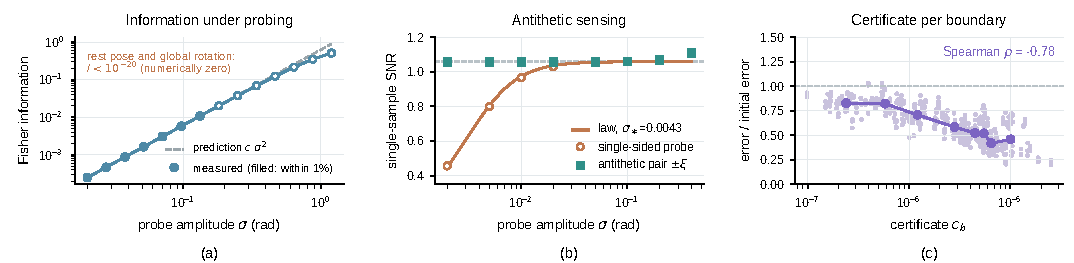
\includegraphics[width=\textwidth]{figure/sysid_checks.pdf}
\caption{\rev{\textbf{Checks of Propositions 1--3.} (a) Fisher information about the boundary of a
two-segment cylinder against the probe amplitude: a relative bend follows the first-order prediction
$c\,\sigma^{2}$ of Proposition~2 (filled markers: within 1\%), while the rest pose and a global
rotation carry none. (b) Single-sample SNR of the sensing estimate on a smooth observation model with
a closed-form posterior: a single-sided probe follows Eq.~\ref{Eq.snr} with $\sigma_{\ast}=0.0043$\,rad,
an antithetic pair is independent of $\sigma$. (c) Boundary error after identification, relative to
the initialisation, against the certificate $c_{b}$ on the Mixamo test characters with motion-prior
probes; dots are boundaries, the line gives means over octiles of $c_{b}$ with standard errors.}}
\label{fig:sysid_checks}
\end{figure*}

\begin{revblock}
\textbf{Second-order sensing.} We verify the estimator of Sec.~\ref{sec:sensor} with SD1.5
\cite{rombach2022high} as the prior. Both ingredients are necessary: the gradient of the
objective of Eq.~\ref{Eq.second} with respect to a scalar boundary parameter has magnitude
$20.2$, and drops to $1.4\times10^{-7}$ without motion ($\sigma=0$) and to $4.0\times10^{-7}$
with a flat prior. On a smooth observation model with a closed-form posterior, the law of
Eq.~\ref{Eq.snr} fits the measured single-sample SNR with $\sigma_{\ast}=0.0043$\,rad and
$\mathrm{SNR}_{\infty}=1.06$ (maximum absolute error $0.010$), and the SNR of the antithetic
estimator does not depend on $\sigma$ (log--log slope $2\times10^{-4}$; Fig.~\ref{fig:sysid_checks}(b)). Reading the posterior
covariance with forward passes only costs $0.033$\,s and $0.18$\,GB per covariance--vector
product, against $0.058$\,s and $0.93$\,GB when back-propagating through the denoiser.

\textbf{Sensor benchmark.} Whether a prior can act as the sensor is tested against artist rigs.
For each limb (an arm or a leg; on RigNet, a chain of three joints) the same deformation is
produced in three ways and the sensor has to pick the correct one, so chance is $1/3$. In the
\textit{hinge} task the limb is bent by the same angle at the true joint, at the midpoint of the
upper segment, or at the midpoint of the lower segment: it asks \textit{where along a limb} a
boundary lies. In the \textit{partition} task the limb is rotated about its proximal joint, and
the moving set is the artist partition, the partition without its distal part (hand or foot),
or the partition enlarged by the parent-side vertices within half a segment length of the
joint: it asks \textit{which vertices move with which handle}. For the articulation prior we also
report the hinge task with angles rescaled to equal RMS displacement, which removes the
magnitude cue. 2D priors observe a rendered crop around the limb under $\pm$ rotations; the
articulation prior observes the deformed points. We use the 43 textured characters, the 30
Mixamo test characters and the RigNet test split, and exclude limbs whose band is empty or whose
distal part has no vertex, on which the three candidates coincide. SD1.5 configurations were
chosen on the first 15 textured characters, and the Wan2.2 entries are the best of all readouts,
i.e.\ optimistic. The noise band of the articulation prior was chosen on the
hinge task with Mixamo and the first 100 RigNet test characters, so that its RigNet entries
are on the remaining 169 characters, and no partition result was seen before either choice.

\textbf{Results.} Table~\ref{table:sensor} separates the two tasks. No prior locates a boundary
along a limb reliably. The best 2D sensor, Qwen3-VL-235B, reaches $0.43$ $[0.35,0.50]$ with only
38\% of its single answers correct, and the articulation prior reaches $0.33$--$0.42$
($0.39$--$0.50$ with matched displacement). The diffusion priors fail in a consistent direction,
towards the candidate that moves the least: on held-out limbs SD1.5 picks the lower midpoint
most often, Wan2.2 with the ELBO picks it on 77 of 80 limbs, and the articulation prior read at
high noise ($t\geq500$) picks it on 207 of 268 RigNet limbs, an accuracy of $0.11$. On the
characters used to fix its band the low-noise readout reached $0.58$ on RigNet, which did not
carry over to the held-out characters ($0.36$). A 2D pose detector \cite{yang2023dwpose} fares
no better: when the joint is moved along the limb to $0.35$ or $0.65$ of its length by a
piecewise-linear stretch, so that guessing the midpoint fails, the keypoint detected on the
static rendering follows the moved joint with a slope of $0.26$ untextured and $0.12$ textured
($1$ is perfect following; SD1.5: $-0.05$ and $-0.04$). The partition, in contrast, is
observable. The articulation prior with the low-noise readout picks the correct partition with
accuracy $0.86$, $0.91$ and $0.92$ on the textured, Mixamo and RigNet limbs, the last including
non-human characters. On the same limbs SD1.5 with the ELBO reaches $0.62$ (textured) and $0.74$
(Mixamo, untextured), and the articulation prior is better on both (paired McNemar test,
$p<10^{-4}$); the classifier score of SD1.5 gives $0.34$ and $0.45$, and Wan2.2 at most $0.45$.
The likelihood ratio against a background model lowers the articulation prior to
$0.52$, $0.73$ and $0.63$. This is the division of labour of Sec.~\ref{sec:sensor}:
the prior senses the partition, and the position of a boundary within a segment is left to the
geometric term.
\end{revblock}

\begin{table*}[t]
  \centering
  \color{red}
  \setlength{\abovecaptionskip}{0.5mm}
  \setlength{\tabcolsep}{3pt}
  \renewcommand{\arraystretch}{1.25}
  \scriptsize
  \caption{\rev{\textbf{Which prior can act as the sensor.} Accuracy of picking the correct one of
  three candidates (chance $0.33$). \textit{Hinge}: the same bend at the true joint or at the
  midpoint of the upper or lower segment, i.e.\ where along a limb a boundary lies; for the
  articulation prior, equal angles / angles matched in RMS displacement. \textit{Partition}: the
  same rotation applied to the artist partition, to the partition without its distal part, or to
  the partition with a leak into the parent part, i.e.\ which vertices move with which handle.
  Brackets: 95\% bootstrap intervals over characters. $^{\dagger}$Data used to choose the
  configuration (first 15 textured characters, or the data used to fix the noise band);
  $^{\ddagger}$all 269 RigNet test characters, degenerate limbs not excluded; all other entries
  are held out. Wan2.2: best of 12 readouts on 20 textured characters.}}
  \label{table:sensor}
  \begin{tabular*}{\textwidth}{@{\extracolsep{\fill}} l c c c c c c}
    \toprule[1.5pt]
    & \multicolumn{3}{c}{\textbf{Hinge}} & \multicolumn{3}{c}{\textbf{Partition}} \\
    \cmidrule(lr){2-4} \cmidrule(lr){5-7}
    \textbf{Sensor} & \textbf{Textured} & \textbf{Mixamo} & \textbf{RigNet} & \textbf{Textured} & \textbf{Mixamo} & \textbf{RigNet} \\
    \midrule[0.5pt]
    SD1.5 \cite{rombach2022high}, full body, untextured & 0.30$^{\dagger}$ & -- & -- & -- & -- & -- \\
    SD1.5, limb crop, untextured                        & 0.45$^{\dagger}$ & -- & -- & -- & 0.74 [0.64, 0.83] & -- \\
    SD1.5, limb crop, textured                          & 0.27 [0.18, 0.38] & -- & -- & 0.62 [0.52, 0.72] & -- & -- \\
    SD1.5, diptych (rest $|$ bent), textured            & 0.33$^{\dagger}$ & -- & -- & -- & -- & -- \\
    Qwen3-VL-8B \cite{qwen3vl2025}, token probabilities & 0.11 [0.06, 0.17] & -- & -- & -- & -- & -- \\
    Qwen3-VL-235B, short reasoning                      & 0.43 [0.35, 0.50] & -- & -- & -- & -- & -- \\
    Qwen3-VL-235B, with rest image                      & 0.35 [0.28, 0.43] & -- & -- & -- & -- & -- \\
    Wan2.2-TI2V-5B \cite{wan2025wan}, 17-frame clip     & $\leq$0.36 & -- & -- & $\leq$0.45 & -- & -- \\
    \midrule[0.5pt]
    Articulation prior, all $t$                         & 0.20 / 0.37 & 0.34 / 0.39 & 0.25 / 0.29$^{\ddagger}$ & -- & -- & -- \\
    Articulation prior, low $t$ (ours)                  & 0.33 / 0.50 & 0.42$^{\dagger}$ / 0.48$^{\dagger}$ & 0.36 / 0.39 & \textbf{0.86} [0.77, 0.94] & \textbf{0.91} [0.77, 0.97] & \textbf{0.92} [0.89, 0.95] \\
    Articulation prior, likelihood ratio                & 0.29 / 0.28 & 0.31$^{\dagger}$ / 0.34$^{\dagger}$ & 0.22 / 0.34 & 0.52 [0.42, 0.62] & 0.73 [0.65, 0.85] & 0.63 [0.56, 0.68] \\
    \bottomrule[1.5pt]
  \end{tabular*}
\end{table*}

\begin{revblock}
\textbf{Amortisation.} Table~\ref{table:amortise} evaluates Sec.~\ref{sec:amortise} on the 269
RigNet test characters \cite{xu2020rignet} with the exact sensor. All predictors except the
conference version receive the mesh and the skeleton, and all are scored on the same boundaries.
The conference version of the Mesh
Handle Predictor does not transfer to heterogeneous skeletons: its 30 skeleton-free parts cannot
be aligned with 9--48 joints, and even with artist supervision it reaches $0.455$, no better than
the geometric initialisation ($0.452$). The pair scorer of Sec.~\ref{sec:amortise} does not
depend on the number or the order of the joints. Trained on the teacher's pseudo-labels of the
2,159 training characters, without any artist annotation, it lowers the error of the geometric
initialisation to $0.375$ in 5\,ms, against $0.311$ with artist supervision and $0.227$ for the
510\,ms teacher. Refining its output with the teacher's objective closes the gap: 30 steps
(27\,ms) give $0.212$ and 100 steps (84\,ms) give $0.190$, below the teacher, which runs 600
steps from the geometric initialisation. On the boundaries that the probes never excite the
refined student reaches $0.312$ against $0.373$ for the teacher; the information there comes
from the other training characters, not from the probes. The same refinement applied to three
published skinning predictors given the ground-truth skeleton, UniRig \cite{zhang2025unirig},
RigAnything \cite{liu2025riganything} and Puppeteer \cite{song2026puppeteer}, lowers their
error from $0.285$--$0.373$ to $0.181$--$0.194$. After 100 steps the starting point therefore
matters little, while at 10 steps a better start still pays off (Puppeteer: $0.229$). The
refinement is thus a complement to any feed-forward rigger, and the student's contribution is
that it needs no artist annotation. Weighting the pseudo-labels by their certificates ($0.377$)
or thresholding them ($0.383$) brings no gain and is not used. Two observations point to noisy
pseudo-labels on part of the non-human assets: a student trained on the 898 human characters
alone reaches $0.377$ on non-human test characters, better than one trained on the 1,261
non-human characters ($0.394$), and the error stops decreasing after 300 training characters
($0.396$, $0.361$, $0.361$ and $0.375$ for 100, 300, 1,000 and 2,159).
\end{revblock}

\begin{table*}[t]
  \centering
  \color{red}
  \setlength{\abovecaptionskip}{0.5mm}
  \setlength{\tabcolsep}{3pt}
  \renewcommand{\arraystretch}{1.25}
  \scriptsize
  \caption{\rev{\textbf{Amortised identification on RigNet} (269 test characters, exact sensor).
  Boundary error (lower is better) on all, human and non-human characters, part IoU and inference
  time of each predictor, and boundary error after $k$ refinement steps of Eq.~\ref{Eq.teacher}
  warm-started from its output (12, 27 and 84\,ms for $k=10,30,100$; part IoU at $k=100$ in
  parentheses). Students: mean $\pm$ std over 2--3 seeds; refinement starts from one seed of the
  pseudo-label student ($0.382$). The external predictors are given the ground-truth skeleton;
  they were trained on large artist-rigged collections that may contain RigNet assets.}}
  \label{table:amortise}
  \begin{tabular*}{\textwidth}{@{\extracolsep{\fill}} l l c c c c c c c c}
    \toprule[1.5pt]
    \textbf{Predictor} & \textbf{Supervision} & \textbf{All} & \textbf{Human} & \textbf{Non-human} &
    \textbf{IoU} & \textbf{Time} & $\bm{k}$\textbf{=10} & $\bm{k}$\textbf{=30} & $\bm{k}$\textbf{=100} \\
    \midrule[0.5pt]
    Geometric initialisation                   & none                 & 0.452 & 0.459 & 0.439 & 0.325 & --      & --    & --    & --    \\
    Teacher, Eq.~\ref{Eq.teacher} (600 steps)  & none                 & \textbf{0.227} & 0.225 & 0.231 & \textbf{0.759} & 510\,ms & -- & -- & -- \\
    TapMo \cite{ICLR2024_94154162}, $K=30$     & pretrained           & 0.539 & 0.507 & 0.598 & 0.340 & 5\,ms   & --    & --    & --    \\
    Student                                    & artist weights       & 0.311$\pm$0.009 & 0.294 & 0.341 & 0.609 & 5\,ms & -- & -- & -- \\
    Student                                    & pseudo-labels        & 0.375$\pm$0.005 & 0.371 & 0.382 & 0.569 & 5\,ms & 0.284 & 0.212 & 0.190 \\
    Student                                    & certificate-weighted & 0.377$\pm$0.007 & 0.373 & 0.385 & 0.553 & 5\,ms & -- & -- & -- \\
    Student                                    & hard threshold       & 0.383 & 0.378 & 0.391 & 0.531 & 5\,ms   & --    & --    & --    \\
    \midrule[0.5pt]
    UniRig \cite{zhang2025unirig}              & artist rigs          & 0.373 & 0.359 & 0.398 & 0.462 & --      & 0.304 & 0.222 & \textbf{0.181} (0.784) \\
    RigAnything \cite{liu2025riganything}      & artist rigs          & 0.368 & 0.356 & 0.390 & 0.559 & --      & 0.276 & 0.208 & 0.184 (\textbf{0.806}) \\
    Puppeteer \cite{song2026puppeteer}         & artist rigs          & 0.285 & 0.274 & 0.304 & 0.601 & --      & \textbf{0.229} & \textbf{0.201} & 0.194 (0.758) \\
    \bottomrule[1.5pt]
  \end{tabular*}
\end{table*}

\begin{revblock}
\textbf{Closing the loop with the prior sensor.} The results above observe the deformed vertices.
Table~\ref{table:e2e} removes every observation of motion: the teacher of Eq.~\ref{Eq.teacher}
is replaced by the minimisation of the sensing objective of Eq.~\ref{Eq.sense} under the
articulation prior, with eight single-joint probes per step, each rotating a random joint by
$\pm(0.5$--$1.2)$\,rad, the low-noise readout, 300 Adam steps and the prior term of
Eq.~\ref{Eq.teacher}; the weight of the sensing term was chosen on 8 of the first 100 RigNet test
characters, and the table reports the remaining 169. From the geometric initialisation the prior
sensor lowers the boundary error from $0.458$ to $0.402$ (paired difference
$-0.057\pm0.006$, lower for 136 of the 169 characters) and raises the part IoU from $0.32$ to
$0.38$; the gain is larger on human ($0.472$ to $0.385$) than on non-human characters ($0.443$
to $0.421$), and it carries over to Mixamo ($0.352$ to $0.298$) and to the textured set ($0.338$
to $0.303$). Distilling the prior teacher over 400 training characters gives a predictor that
needs neither artist rigs nor observed motion, $0.409$ in 5\,ms, and $0.395$ after the same
prior refinement. Starting from the student trained on exact-sensor pseudo-labels, the prior
refinement lowers the error from $0.394$ to $0.341$ (lower for 147 of 169) but also lowers the
IoU, because it moves weight across boundaries without the evidence to locate them along the
limb. The prior sensor thus recovers about a quarter of the gap between the geometric
initialisation and the exact-sensor teacher ($0.227$), which is the price of removing every
observation of the moving character.
\end{revblock}

\begin{table*}[t]
  \centering
  \color{red}
  \setlength{\abovecaptionskip}{0.5mm}
  \setlength{\tabcolsep}{3pt}
  \renewcommand{\arraystretch}{1.25}
  \scriptsize
  \caption{\rev{\textbf{Identification without any observation of motion.} Boundary error of the
  articulation-prior sensor used as the only sensor (Eq.~\ref{Eq.sense}), on 169 held-out RigNet
  test characters, the 30 Mixamo test characters and the 43 textured characters; the exact-sensor
  teacher is the reference that observes the deformed vertices. ``Observations'' lists what each
  row needs beyond the rest mesh and its skeleton.}}
  \label{table:e2e}
  \begin{tabular*}{\textwidth}{@{\extracolsep{\fill}} l l c c c c c c c}
    \toprule[1.5pt]
    & & \multicolumn{5}{c}{\textbf{RigNet (held out)}} & \textbf{Mixamo} & \textbf{Textured} \\
    \cmidrule(lr){3-7}
    \textbf{Method} & \textbf{Observations} & \textbf{All} & \textbf{Human} & \textbf{Non-human} & \textbf{Worst} & \textbf{IoU} & \textbf{All} & \textbf{All} \\
    \midrule[0.5pt]
    Geometric initialisation                      & none                     & 0.458 & 0.472 & 0.443 & 0.704 & 0.32 & 0.352 & 0.338 \\
    Prior sensor, from the geometric initialisation & none                   & 0.402 & 0.385 & 0.421 & 0.661 & 0.38 & \textbf{0.298} & \textbf{0.303} \\
    Student distilled from the prior sensor       & none                     & 0.409 & 0.397 & 0.424 & 0.643 & 0.35 & --    & --    \\
    \quad $+$ prior refinement                    & none                     & 0.395 & 0.375 & 0.417 & 0.679 & 0.36 & --    & --    \\
    \midrule[0.5pt]
    Student, exact-sensor pseudo-labels           & vertices, training only  & 0.394 & 0.396 & 0.393 & 0.608 & 0.53 & --    & --    \\
    \quad $+$ prior refinement                    & vertices, training only  & 0.341 & 0.330 & 0.353 & 0.585 & 0.49 & --    & --    \\
    Exact-sensor teacher, Eq.~\ref{Eq.teacher}    & vertices of every probe  & \textbf{0.227} & \textbf{0.230} & \textbf{0.223} & \textbf{0.457} & \textbf{0.76} & -- & -- \\
    \bottomrule[1.5pt]
  \end{tabular*}
\end{table*}

\begin{revblock}
\textbf{Sensing on generated meshes.} Because the sensing term acts on the field only, it can be
applied to any generated mesh, for which no motion can be observed. We take the meshes that
Hunyuan3D-2mini produces from the T-pose-conditioned and from the unconditioned images of
Table~\ref{table:interaction}, and that Hunyuan3D~2.1, TripoSG and TRELLIS produce from the
T-pose-conditioned ones (80 meshes, post-processed as in Sec.~\ref{3Dmesh}), and identify the field
of our animator with the articulation prior as the only sensor, starting from the predicted field
and following the protocol of Table~\ref{table:e2e} with handles in place of joints. Driven by the
same generated motions (4 held-out prompts), the identified field lowers the failure rate of our
animator from 28.1\% to 20.3\% ($-7.8$ points, 95\% interval $[-12.8,-3.1]$ over characters) and
its self-intersection by $1.7$ points ($[-2.4,-1.1]$, significant on each of the five mesh sets);
the length-weighted edge change falls from $0.087$ to $0.077$ and the bending from $5.3^{\circ}$ to
$4.9^{\circ}$, while the mean vertex displacement falls by only 3\%. The mean squared edge-length
change, in contrast, rises from $0.37$ to $0.60$ ($\times10^{-4}$): the identified field
concentrates the remaining deformation on fewer edges. The identification uses neither an artist
rig nor an observed motion of the character, and, unlike Table~\ref{table:e2e}, the test is scored
on the animation itself rather than against artist weights. The same holds on non-human characters, for which no text--motion pairs are used in training. For 12 non-human prompts (dog, horse, fox, elephant, winged dragon, eagle, shark, spider, crab, T-rex, frog and turtle) we take the meshes of TRELLIS, generated from an SD1.5 image of each prompt, and those of our generator of Table~\ref{table:gengrid}, initialised in a sphere since the T-pose body does not apply, with and without the coupling terms (36 meshes, the same 4 held-out motions). The sensing term lowers the failure rate of our animator from 48.6\% to 34.7\% ($-$13.9 points, $[-22.2,-6.3]$), its self-intersection by 2.2 points ($[-3.1,-1.5]$), the length-weighted edge change from 0.104 to 0.087 and the bending from $6.1^{\circ}$ to $4.7^{\circ}$; the failure rate falls on each of the three mesh sets, on the TRELLIS meshes from 37.5\% to 22.9\% and on those of our generator from 54.2\% to 39.6\%. Fig.~\ref{fig:gen_nh} shows, for each of the two generators, the two clips whose distortion falls most.
\end{revblock}

\begin{figure*}[t]
\centering
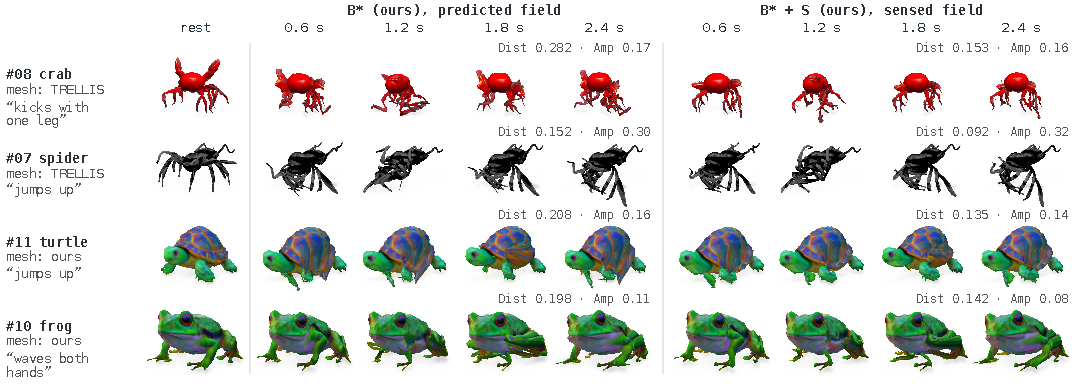
\includegraphics[width=\textwidth]{figure/gen_nh.pdf}
\caption{\rev{\textbf{Sensing on non-human characters.} For each generator (TRELLIS from an SD1.5 image of
the prompt; ours initialised in a sphere, with both coupling terms), the two clips (character and
held-out prompt) whose Dist.\ falls most under the sensing term. Left: our animator with the predicted
field; right: the same motion samples with the field identified by the sensing term, with the
articulation prior as the only sensor and no observed motion of the character. Dist.\ and Amp.\ as in
Fig.~\ref{fig:gen_e2e}.}}
\label{fig:gen_nh}
\end{figure*}

\begin{revblock}
\textbf{Excitation in the motion model.} Table~\ref{table:pe} tests the objective of
Eq.~\ref{Eq.lpe} in two forms. The first is an amortised design head: a per-joint MLP that maps
the character to a diagonal probe covariance under the budget and the cap of Eq.~\ref{Eq.sdp}
($\kappa=4$), for the non-uniform motion prior of Table~\ref{table:sysid}. It is trained on 596
RigNet training characters and evaluated by identifying the 269 test characters from 8 probes
drawn from its design. Decreasing $\lambda$ trades fidelity to the prior for identifiability
monotonically; at $\lambda=0.01$ the mean error falls from $0.276$ to $0.234$ and the worst
boundary from $0.505$ to $0.435$, with $0.233$ and $0.236$ on human and non-human characters. The
per-character max--min design, restricted to the same diagonal covariances, puts the budget on a
few joints (KL $159$) and is worse than the prior in both mean and worst error, which is why
Eq.~\ref{Eq.lpe} uses a soft-min. The second form guides the pretrained Shape-aware Motion
Diffusion with Eq.~\ref{Eq.guide}, without retraining. $I_{b}$ is computed on the boundaries of
the initial, geometric field, and the generated motions serve as probes to identify the 30-handle
skinning of the Mesh Handle Predictor from noisy vertices. The weakest-boundary information grows
up to $5.1\times$ and the identification error falls monotonically with $\eta$, by 12\% in mean
and 8\% in worst boundary at $\eta=0.2$, while the jerk is almost unchanged. Against the unguided
sample with the same noise, the error on the boundaries present in the initial field falls for all
30 character--seed pairs at $\eta\geq0.1$. The cost is a departure from the text-conditioned
samples that grows linearly with $\eta$ ($0.065$ at $\eta=0.05$, $0.248$ at $\eta=0.2$). The
boundaries absent from the initial field, which the guidance cannot target, also improve
($0.282$ to $0.249$). This is not an effect of larger motion: the guided motions are only 2.7\%
larger in mean squared displacement, and unguided motions rescaled to the same amplitude lower
the error by $0.002$ instead of $0.022$. Guidance along random directions with the same step,
however, lowers the error much further ($0.188$ to $0.030$ at $\eta=0.2$) at a similar
departure from the unguided samples, but with $5.7\times$ the jerk. As with the isotropic design
of Table~\ref{table:sysid}, dithering every handle is the stronger excitation when the probes
only have to be observed; $\mathcal{L}_{\text{PE}}$ is the choice when the probes must stay
smooth motions close to the text-conditioned distribution, for instance when the motions that
identify the field are also the ones shown to the user. Text fidelity, measured with a
text--motion evaluator that we retrain for the 30-handle representation following the protocol
of \cite{guo2022generating} (R@3 $0.774$ on real test motions), decreases only slightly under
$\mathcal{L}_{\text{PE}}$ guidance (R@3 $0.704$ to $0.676$ at $\eta=0.2$) and is unchanged under
random dithering ($0.701$), whose jerk the evaluator does not penalise. Fine-tuning the motion
model by reward-weighted regression \cite{peters2007reinforcement}, with the soft-min of
Eq.~\ref{Eq.lpe} as the reward, raises the reward on the training characters ($-10.12$ to
$-9.78$ over two rounds) but does not transfer to the test characters: the identification error
rises slightly ($0.188$ to $0.195$) and the samples move far from those of the original model
(Dev. $0.77$). Identifiability is therefore obtained at sampling time, not by this fine-tuning.
\end{revblock}

\begin{table*}[t]
  \centering
  \color{red}
  \setlength{\abovecaptionskip}{0.5mm}
  \renewcommand{\arraystretch}{1.25}
  \scriptsize
  \caption{\rev{\textbf{The excitation objective $\mathcal{L}_{\text{PE}}$} of Eq.~\ref{Eq.lpe}.
  (a) Amortised design head on RigNet (269 test characters, 8 probes, 2 seeds): boundary error,
  information of the weakest boundary relative to the motion prior, KL divergence from the prior
  and time per character. (b) The pretrained motion diffusion model, guided by Eq.~\ref{Eq.guide},
  guided along random directions with the same step, or fine-tuned by reward-weighted regression
  (15 Mixamo test characters $\times$ 16 HumanML3D test prompts $\times$ 2 seeds; initial field
  $0.463$): identification error from the generated motions on all boundaries, on the boundaries
  present in the initial field and on those absent from it; RMSE to the unguided sample with the
  same noise (Dev., normalised feature units); mean jerk of the handle trajectories; R-precision
  (top 3 of 32) and FID of a text--motion evaluator retrained for the 30-handle representation,
  on 4 characters $\times$ 64 test prompts (real test motions: R@3 $0.774$).}}
  \label{table:pe}
  \begin{tabular*}{\textwidth}{@{\extracolsep{\fill}} l c c c c c}
    \toprule[1.5pt]
    \textbf{(a) Design} & \textbf{Mean} & \textbf{Worst} & \textbf{Weakest info.} & \textbf{KL} & \textbf{Time} \\
    \midrule[0.5pt]
    Motion prior (no $\mathcal{L}_{\text{PE}}$)            & 0.276 & 0.505 & 1.00$\times$ & 0    & --      \\
    Head, $\lambda=1$                                      & 0.275 & 0.503 & 1.06$\times$ & 0.03 & 2.5\,ms \\
    Head, $\lambda=0.1$                                    & 0.262 & 0.479 & 1.83$\times$ & 3.7  & 2.5\,ms \\
    Head, $\lambda=0.01$                                   & \textbf{0.234} & \textbf{0.435} & 3.05$\times$ & 26 & 2.9\,ms \\
    Head, $\lambda=0$                                      & \textbf{0.234} & \textbf{0.435} & 3.05$\times$ & 30 & 3.1\,ms \\
    Per-character max--min (Eq.~\ref{Eq.sdp}, diagonal)    & 0.311 & 0.527 & 3.57$\times$ & 159  & 1.4\,ms \\
    \bottomrule[1.5pt]
  \end{tabular*}
  \vspace{1mm}

  \begin{tabular*}{\textwidth}{@{\extracolsep{\fill}} l c c c c c c c c c}
    \toprule[1.5pt]
    \textbf{(b) Motion model} & \textbf{Mean} & \textbf{Worst} & \textbf{Present} & \textbf{Absent} &
    \textbf{Weakest info.} & \textbf{Dev.} & \textbf{Jerk} & \textbf{R@3}$_{\uparrow}$ & \textbf{FID}$_{\downarrow}$ \\
    \midrule[0.5pt]
    $\eta=0$ (original sampler) & 0.188 & 0.472 & 0.108 & 0.282 & 1.0$\times$ & 0     & 0.0057 & 0.704 & 0.277 \\
    $\eta=0.02$                 & 0.185 & 0.469 & 0.107 & 0.276 & 2.5$\times$ & 0.027 & 0.0058 & --    & --    \\
    $\eta=0.05$                 & 0.180 & 0.465 & 0.103 & 0.271 & 2.6$\times$ & 0.065 & 0.0058 & 0.698 & 0.269 \\
    $\eta=0.1$                  & 0.175 & 0.456 & 0.100 & 0.262 & 3.0$\times$ & 0.126 & 0.0058 & 0.692 & 0.256 \\
    $\eta=0.2$                  & 0.166 & 0.432 & 0.092 & 0.249 & 5.1$\times$ & 0.248 & 0.0060 & 0.676 & 0.233 \\
    \midrule[0.5pt]
    Unguided, rescaled to the amplitude of $\eta=0.2$ & 0.185 & 0.468 & 0.107 & 0.279 & 1.03$\times$ & 0.041 & 0.0058 & -- & -- \\
    Random direction, $\eta=0.1$ & 0.087 & 0.284 & 0.052 & 0.129 & 3.3$\times$ & 0.103 & 0.0179 & 0.704 & 0.276 \\
    Random direction, $\eta=0.2$ & \textbf{0.030} & \textbf{0.102} & \textbf{0.017} & \textbf{0.046} & 8.4$\times$ & 0.206 & 0.0326 & 0.701 & 0.274 \\
    RWR fine-tuned with $\mathcal{L}_{\text{PE}}$ reward, $\eta=0$ & 0.195 & 0.484 & 0.110 & 0.296 & -- & 0.766 & 0.0082 & 0.768 & 0.291 \\
    \bottomrule[1.5pt]
  \end{tabular*}
\end{table*}

\begin{revblock}
\textbf{Which excitation suits which sensor.} Table~\ref{table:probes} identifies the 30 Mixamo
test characters from four probe distributions under both sensors: single-joint rotations,
isotropic dithering of all joints, motion-capture frames, and motion-capture frames selected by the
soft-min information of Eq.~\ref{Eq.lpe} (top 20\% of the frames). With the exact sensor
dithering is best ($0.060$), and the selection by $\mathcal{L}_{\text{PE}}$ improves on random
motion-capture frames ($0.077$ against $0.086$). With the prior sensor the ordering inverts:
dithering brings no gain ($0.357$ against $0.352$ for the initialisation), motion-capture frames
help a little ($0.321$) and single-joint articulations most ($0.297$); the selection by
$\mathcal{L}_{\text{PE}}$ is no better than random frames ($0.327$). The information of
Proposition~2 is that of an exact sensor. A prior sensor can only use probes that resemble the
articulations it was trained on, so excitation for it has to be designed with its own precision,
which Eq.~\ref{Eq.lpe} does not yet do.
\end{revblock}

\begin{table}[t]
  \centering
  \color{red}
  \setlength{\abovecaptionskip}{0.5mm}
  \setlength{\tabcolsep}{3pt}
  \renewcommand{\arraystretch}{1.2}
  \scriptsize
  \caption{\rev{\textbf{Excitation against sensor} (30 Mixamo test characters, geometric
  initialisation $0.352$). Boundary error / worst boundary after identification with the exact
  sensor (8 probes) and with the articulation prior as the only sensor (300 steps $\times$ 16 probes).}}
  \label{table:probes}
  \begin{tabular*}{\linewidth}{@{\extracolsep{\fill}} l c c c c}
    \toprule[1.5pt]
    & \multicolumn{2}{c}{\textbf{Exact sensor}} & \multicolumn{2}{c}{\textbf{Prior sensor}} \\
    \cmidrule(lr){2-3} \cmidrule(lr){4-5}
    \textbf{Probes} & \textbf{Mean} & \textbf{Worst} & \textbf{Mean} & \textbf{Worst} \\
    \midrule[0.5pt]
    Single-joint rotations            & 0.273 & 0.487 & \textbf{0.297} & \textbf{0.550} \\
    Isotropic dithering               & \textbf{0.060} & \textbf{0.110} & 0.357 & 0.703 \\
    Motion capture                    & 0.086 & 0.204 & 0.321 & 0.633 \\
    Motion capture, $\mathcal{L}_{\text{PE}}$-selected & 0.077 & 0.166 & 0.327 & 0.638 \\
    \bottomrule[1.5pt]
  \end{tabular*}
\end{table}

\begin{revblock}
\textbf{Limitations of the added analyses.} Without any observation of motion, the
prior sensor recovers only about a quarter of the gap to the exact-sensor teacher
(Table~\ref{table:e2e}), and on generated meshes the sensing term $\lambda_{5}S$ has been applied to the
field of the extracted mesh rather than inside the joint optimisation of Eq.~\ref{Eq.unified}. The articulation prior senses the partition but not
the position of a boundary along a segment, which is left to the geometric term. The certificate
is computed with the precision of an exact sensor, so it does not reveal this blindness of the
prior. RigNet has no motion capture, so its probes and motion priors are synthetic. The external
riggers of Table~\ref{table:amortise} may have seen RigNet assets during training. In the
motion-guidance experiment the ground truth is the 30-handle field of our own predictor, and the
text--motion evaluator is retrained by us, so its R-precision and FID are comparable only within
Table~\ref{table:pe}. In the stage-interaction experiment of Table~\ref{table:interaction} the
animatability prior refines meshes of an off-the-shelf generator instead of acting on the
Gaussians during generation, Pose-SDS is not tested, and B$_{0}$ is a single system; the
distortion measure is close to the objective of the coupling term, but self-intersection and
bending, which are not optimised, fall as well. Re-measured under one protocol, AnimateAnyMesh distorts less
than our animator on unseen characters (Table~\ref{table:rigfree2}), and the values reported for
it in Table~\ref{table:rigfree} could not be reproduced. The generator of Table~\ref{table:gengrid} is our implementation with the MVDream prior rather than the camera-adapted SDXL generator, and the parameters of its mesh extraction were chosen on 10 of its 16 characters, by the agreement between mesh and Gaussians only.
\end{revblock}

\subsection{User Study}
We conducted a user study to evaluate the visual effects of our TapMeMo against the baseline methods. We invited 100 volunteers and gave them 15 videos. Each video includes one textual description and three anonymous animation results. We ask users to rank the three results in three aspects: overall quality (O-Q), text-motion matching degree (T-M), and geometry quality (G-Q). After excluding abnormal questionnaires, we collect 1,335 ranking comparison statistics in total, and the average rank of the methods is summarized in Table \ref{fig:userstudy}. Our TapMeMo outperforms the baseline methods by a large margin and more than 84\% of users prefer the animation generated by our TapMeMo.
\begin{table}[h]
\centering
\begin{minipage}[h]{0.48\textwidth}
\vspace{0pt} % 确保顶部对齐
\centering
\caption{\textbf{User Study of the animation quality.} We show the average ranking results where the first is the best.}
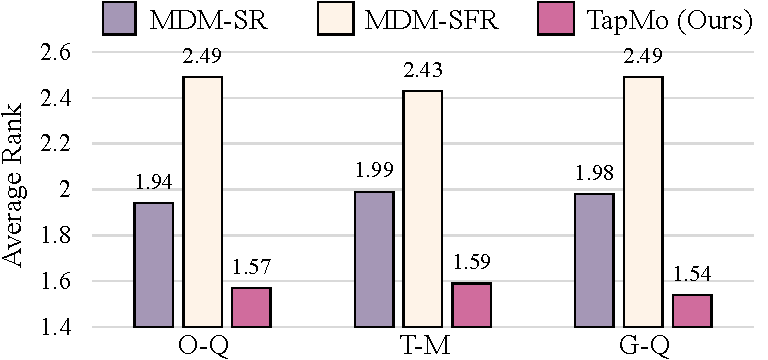
\includegraphics[width=\linewidth]{figure/userstudy.pdf}
\label{fig:userstudy}
\vspace{-0.9cm}
\end{minipage}
\end{table}


\section{Conclusion}
In this work, we propose TapMeMo, a novel text-driven animation pipeline designed to simplify the creation of 3D animations without requiring expert knowledge. TapMeMo eliminates the limitations of traditional skeletal rigs by adopting a fully skeleton-free framework, enabling the generation of pose-aware meshes and mesh-specific motions that maintain geometric integrity and visual fidelity.

Our pipeline is organised around a single shared object rather than a sequence of stages. The handle field assigns every point of space a distribution over a fixed set of deformation channels, and it is read both while the character is being generated and while it is being driven. Characterising when handle-based driving is exact yields three conditions that the generated asset must satisfy, and these conditions are what the generator is built to meet: the canonical rest pose is the unique identity of the driving operator, because blend skinning does not compose; the T-pose initialization fixes the gauge of the handle channels, which the rest-pose rendering objective is provably unable to learn; and a uniform, budgeted triangulation is the quadrature condition under which the discrete handle estimate agrees with its continuous definition. The two coupling terms, pose distillation under generated motion and the animatability prior, then close the loop by routing the generative gradient through the deformation operator, so that the generator is optimised for the animation it will have to support rather than for appearance alone.

To address the scarcity of the paired text-motion data, we adopt a weakly supervised training paradigm, enabling adaptive mesh handle learning and mesh-specific motion generation under limited supervision. Extensive qualitative and quantitative evaluations demonstrate that our exploited TapMeMo surpasses existing auto-animation approaches, producing higher-quality and more coherent animations across a diverse range of characters and prompts.

\begin{revblock}
Sharing the field also makes explicit where its information comes from. The rest-pose objective
carries none, so the field has to be identified from motion: the information is linear in the
probe covariance and non-singular exactly when every part boundary is persistently excited,
which gives each boundary a certificate and gives the motion model an excitation objective.
Among the priors we tested, an articulation prior trained on static 3D data is the one that
senses which vertices move together, on human and non-human characters alike, whereas the
position of a boundary along a limb is observable to none of them and remains a matter of
geometry. Amortised into the predictor and followed by a short refinement, the identification is
more accurate than per-character optimisation, and the same refinement improves published
riggers. Without any observation of motion the prior sensor still improves a geometric rig, by
12\% on held-out characters, and on the meshes of four off-the-shelf generators it lowers the
failure rate of our animator from 28\% to 20\%, and on non-human characters from 49\% to 35\%. The four conditions of the drivable manifold are each tested
by a separate measurement. The factorial test finds no interaction for the rest-pose condition
alone and a significant one once the animatability prior couples the generated geometry to the
animator: the asset improves for our animator and not for another one, which a cascade cannot
produce. The mesh post-processing interacts with the animator in the same way: it lowers the
failure rate of our animator on all four generators tested and improves none of three other
animators consistently. Whether the same holds when the coupling acts on the Gaussians during generation, and
for pose distillation, remains to be measured.
\end{revblock}

In summary, our TapMeMo provides an end-to-end solution for text-driven 3D animation, paving the way for intuitive and flexible character animation generation in both human and non-human domains.

% \section{Conclusion}
% In this work, we propose a novel text-driven animation pipeline called TapMeMo, which enables non-experts to create their own animations without requiring professional knowledge. TapMeMo leverages two key components to control and animate a wide range of skeleton-free characters. The first is the Mesh Handle Predictor, which clusters mesh vertices into adaptive handles for semantic control. The second is Shape-aware Motion Diffusion, which generates text-guided motions while considering the specific deformation properties of the mesh, ensuring coherent and plausible character animation without introducing mesh distortion.

% In addition, we introduce the use of 3D Gaussian to directly generate mesh from images, enabling seamless mesh creation and animation driving. To train TapMeMo with limited ground-truth data of both handle-annotated 3D characters and text-relevant motions, we propose a weakly-supervised training strategy for adaptive mesh handle learning and mesh-specific motion learning. Our extensive experiments validate the effectiveness of our method, and we show that it achieves state-of-the-art performance compared to baseline methods.

\printbibliography

\vspace{0.5cm} 
\begin{IEEEbiography}[{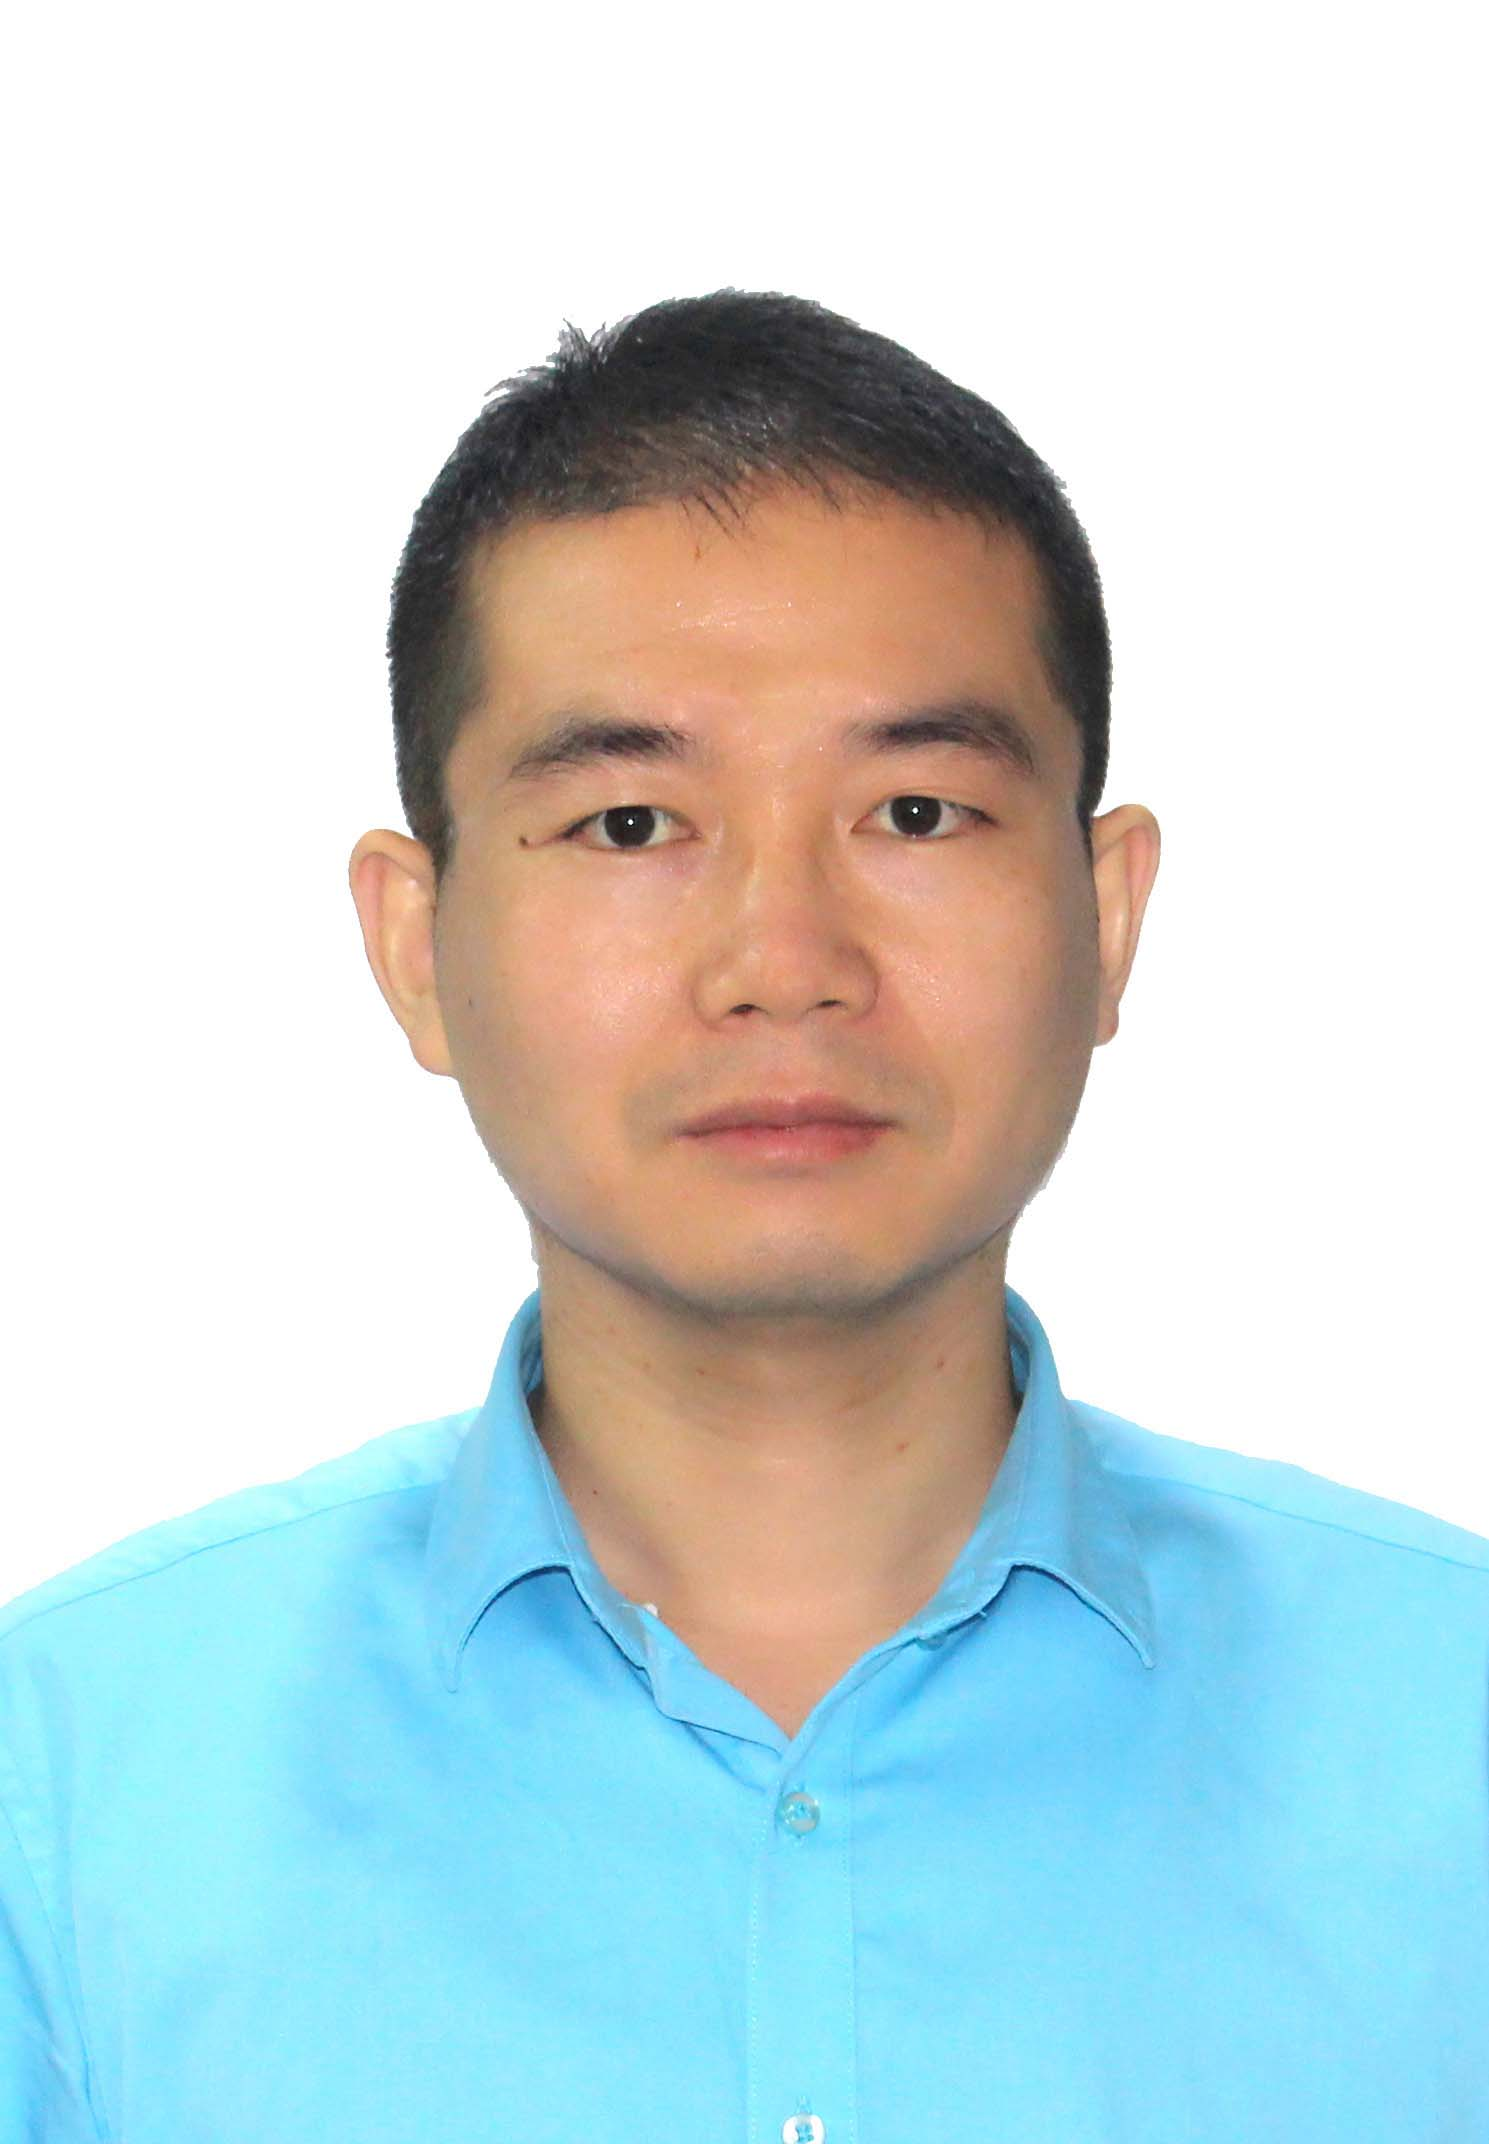
\includegraphics[width=0.95\textwidth]{biofig/ZhigangTu.jpg}}]{\textbf{Zhigang Tu}} (Member, IEEE) received the Ph.D.
degree from Wuhan University, China, in 2013, and the Ph.D. degree from Utrecht University, Netherlands, in 2015. From 2015 to 2016, he was a Postdoctoral Researcher with Arizona State University, USA. From 2016 to 2018, he was a Research Fellow with Nanyang Technological University, Singapore. 

He is currently a Professor with Wuhan University. He has
co-/authored more than 70 papers in international SCI-indexed journals and conferences. His current research interests include computer vision, image processing, video analytics, machine learning, motion estimation, human action and gesture recognition, and anomaly event detection. He is the first organizer of the ACCV2020
Workshop on MMHAU, Japan. He received the Best Student Paper Award at the $4^{th}$ Asian Conference on Artificial Intelligence Technology and one of the three best reviewers awards for \textit{IEEE Transactions on Circuits and Systems for Video Technology (IEEE T-CSVT)} in 2022. He is the Area Chair of AAAI2023/2024 and VCIP2022. He is an Associate Editor of the SCI-indexed journal \textit{The Visual Computer} (IF=3.5) and a Guest Editor of \textit{Journal of Visual Communications and Image Representation} (IF=2.6).
\end{IEEEbiography}

\begin{IEEEbiography}[{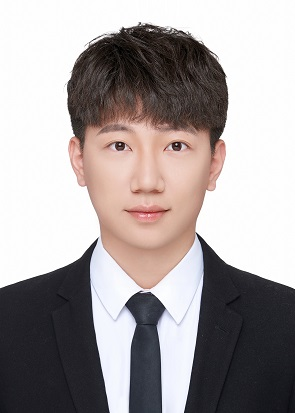
\includegraphics[width=0.95\textwidth]{biofig/wang.jpg}}]
{\textbf{Hequan Wang}} received his B.S. degree from Northeastern University, Shenyang, China, in 2024. He is currently pursuing a M.S. degree at the LIESMARS (State Key Laboratory of Information Engineering in Surveying, Mapping and Remote Sensing), Wuhan University, China. His research interests include computer vision, computer graphics, and motion synthesis.
\end{IEEEbiography}

\begin{IEEEbiography}[{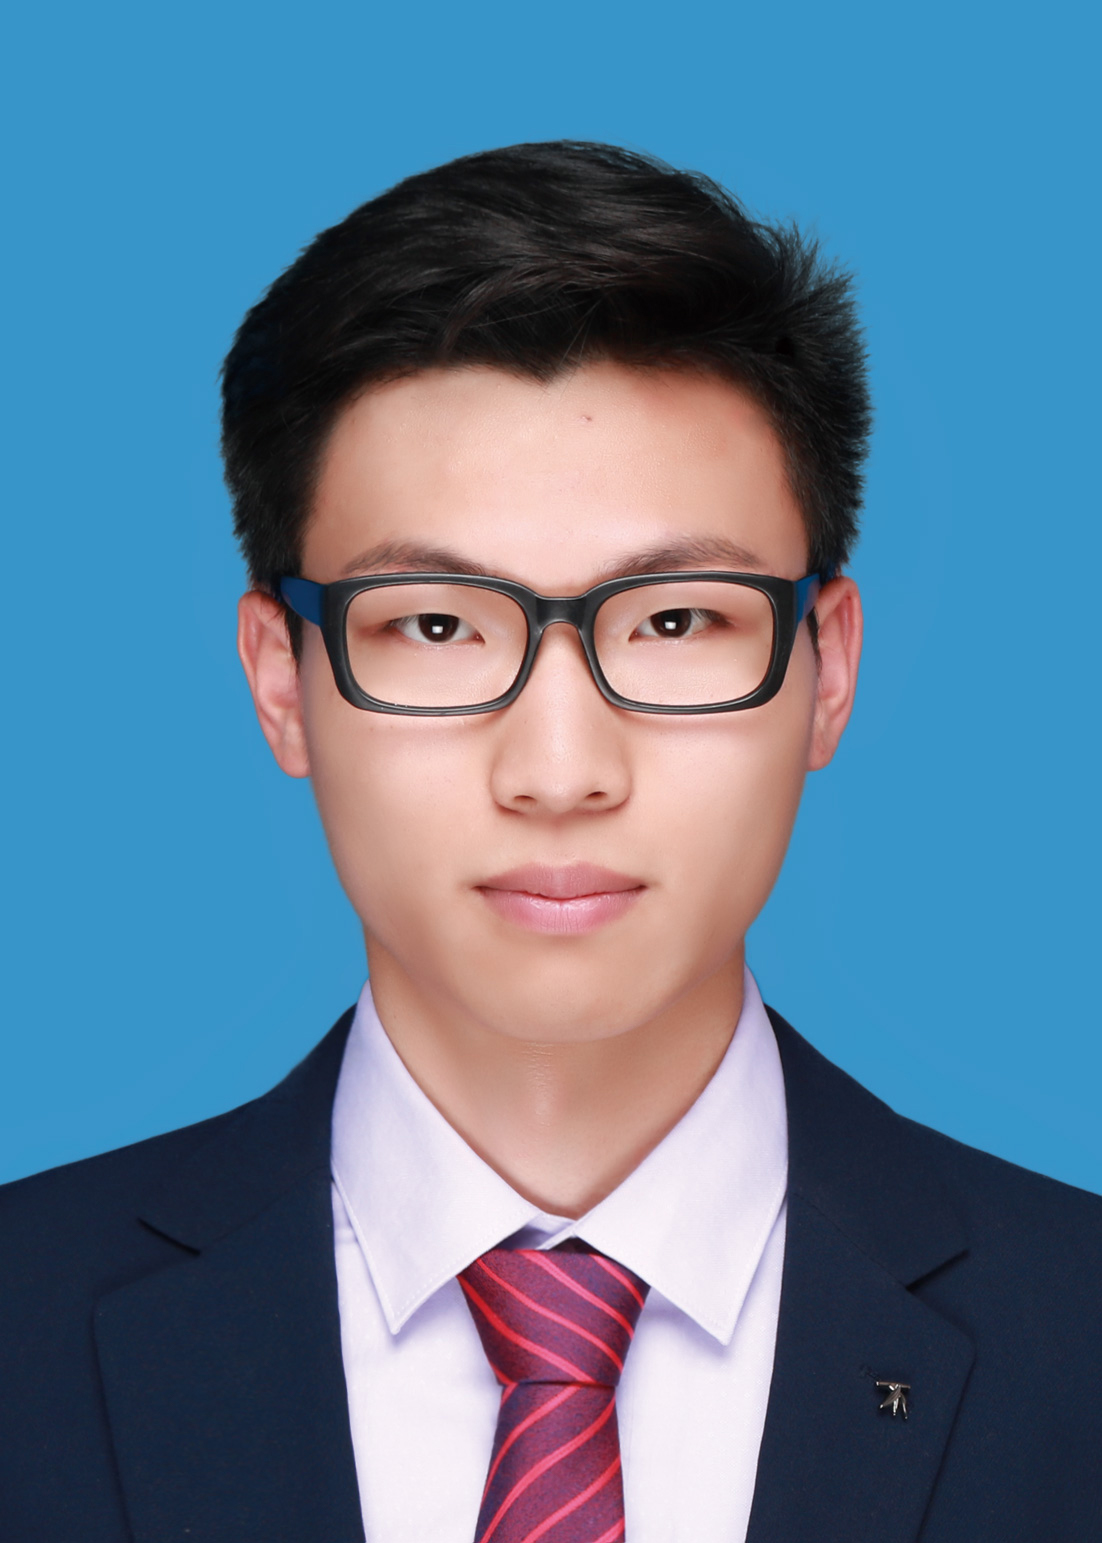
\includegraphics[width=0.95\textwidth]{biofig/zhangjiaxu.jpg}}]
{\textbf{Jiaxu Zhang}} received his B.S. degree from Southeast University, Nanjing, China, in 2020. He is currently working toward a Ph.D. degree at the LIESMARS (State Key Laboratory of Information Engineering in Surveying, Mapping and Remote Sensing), Wuhan University, China. His research interests include computer vision, computer graphics, and motion synthesis.
\end{IEEEbiography}

\begin{IEEEbiography}[{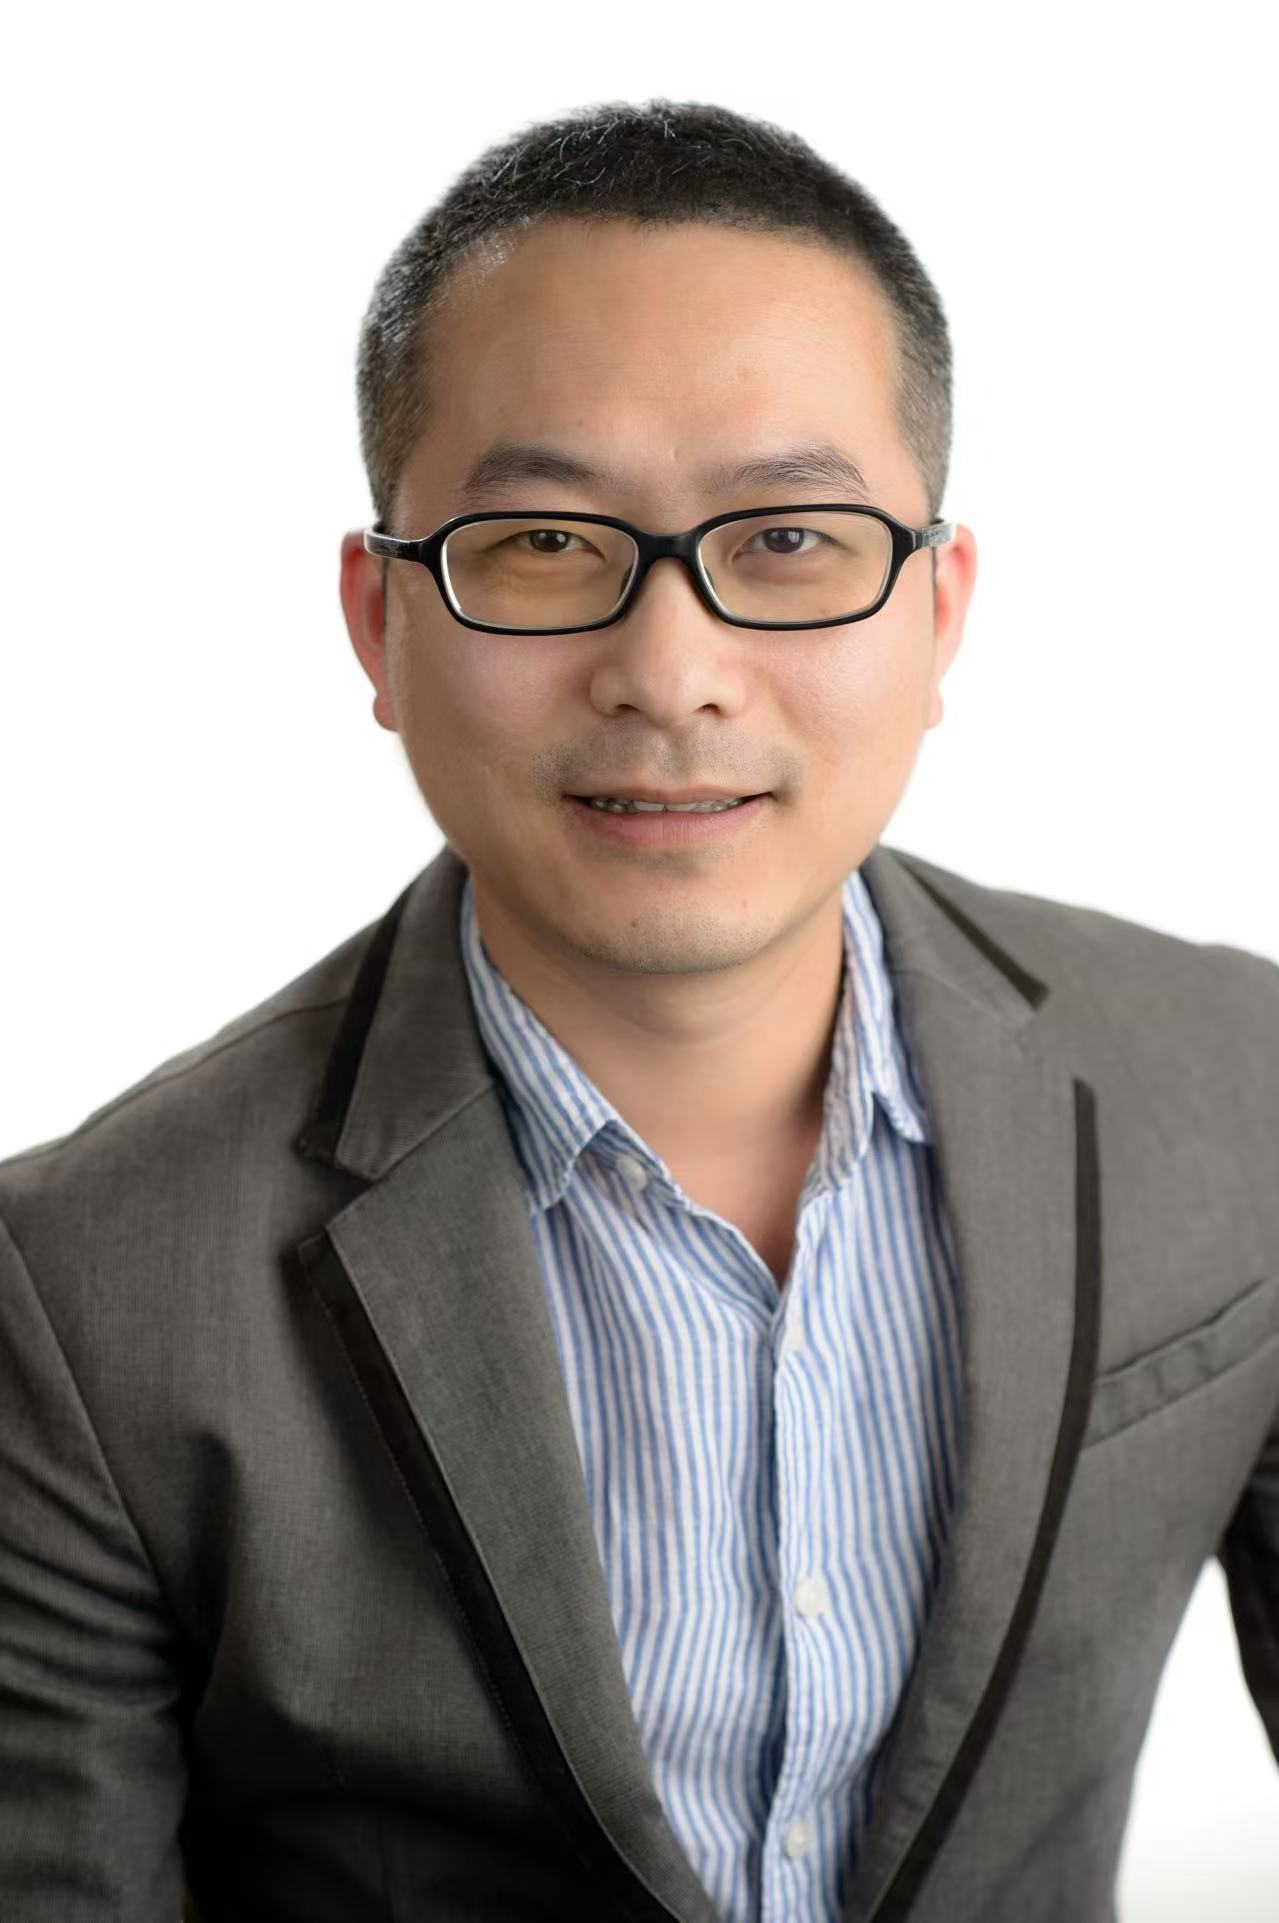
\includegraphics[width=0.95\textwidth]{biofig/huang.jpg}}]
{\textbf{Shaoli Huang}} is a senior researcher at Tencent AI Lab. He obtained the Ph.D. from the University of Technology Sydney under the supervision of Professor Tao Dacheng and later served as a research fellow at the University of Sydney. His research interests emphasize practical applications with a strong focus on digital human and embodied AI technologies, such as video-based human motion capture, motion generation, and motion retargeting.
\end{IEEEbiography}

\begin{IEEEbiography}[{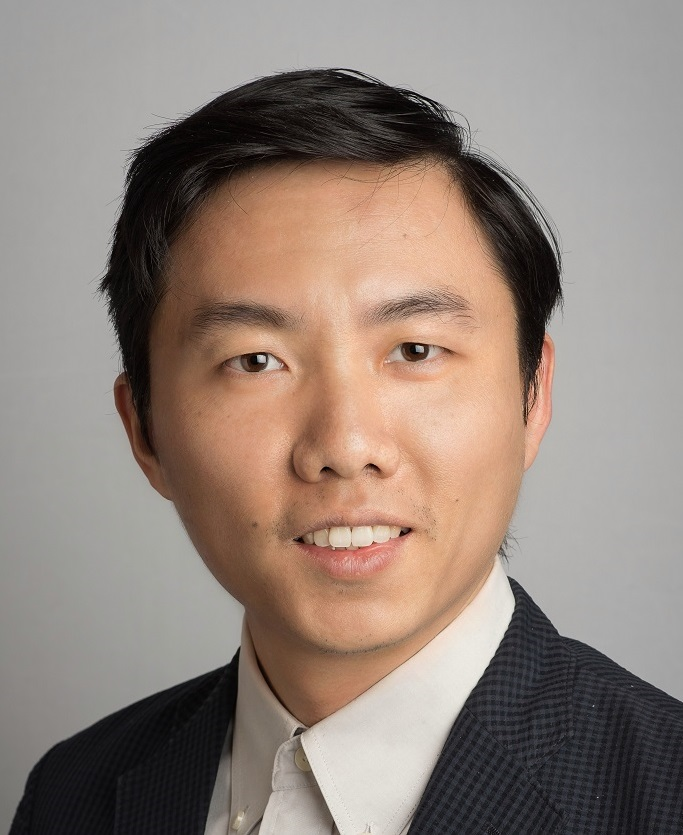
\includegraphics[width=0.95\textwidth]{biofig/Yuan.jpg}}]
{\textbf{Junsong Yuan}} (Fellow, IEEE) is Professor and Director of Visual Computing Lab at Department of Computer Science and Engineering, State University of New York at Buffalo (UB), USA. Before that he was Associate Professor (2015-2018) and Nanyang Assistant Professor (2009-2015) at Nanyang Technological University (NTU), Singapore. He obtained his Ph.D. from Northwestern University in 2009, M. Eng. from National University of Singapore in 2005, and B. Eng. from Huazhong University of Science Technology in 2002. His research interests include computer vision, pattern recognition, video analytics, large-scale visual search and mining. He received Best Paper Award from IEEE Trans. on Multimedia, Nanyang Assistant Professorship from NTU, and Outstanding EECS Ph.D. Thesis award from Northwestern University. 

He served as Associate Editor of IEEE Trans. on Pattern Analysis and Machine Intelligence (TPAMI), IEEE Trans. on Image Process. (TIP), IEEE Trans. on Circuits and Systems for Video Tech. (TCSVT), and Senior Area Editor of Journal of Visual Communications and Image Representation. He was Program Co-Chair of IEEE Conf. on Multimedia Expo (ICME'18/2022/2024), and Area Chair for CVPR, ICCV, ECCV, and ACM MM. He was elected senator at both NTU and UB. He is a Fellow of IEEE and IAPR.
\end{IEEEbiography}


\begin{IEEEbiography}[{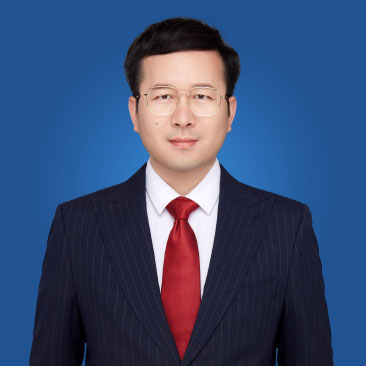
\includegraphics[width=0.95\textwidth]{biofig/BoDu.jpg}}]
{\textbf{Bo Du}} (Senior Member, IEEE) received the Ph.D. degree in photogrammetry and remote sensing from the State Key Laboratory of Information Engineering in Surveying, Mapping and Remote Sensing, Wuhan University, Wuhan, China, in 2010. He is a Professor with the School of Computer Science, Wuhan University. He has over 300 research articles published in the journals of IEEE Transactions on Pattern Analysis and Machine Intelligence (TPAMI), IEEE Transactions on Image Processing (TIP), IEEE Transactions on Geoscience and Remote Sensing (TGRS), ISPRS Journal of Photogrammetry and Remote Sensing, etc. More than 50 of them are ESI hot articles or highly cited articles. His major research interests include pattern recognition, hyperspectral image processing, machine learning, and signal processing.
\end{IEEEbiography}


\end{document}



